% paper_v2_full.tex -- version 2.2 (2026-10-19; Lean tile counts for eight template values, W3+ census as evidence, release v1.16; text of version 2.1 otherwise). Self-contained: own preamble, own bibliography.
% Marks: \sF (Lean theorem), \sW (written proof, not formalized), \sS (computation without a kernel-checked certificate).
% Assembled by private/DRAFT/build_full.py from part files; the Herdt and census sections are patched copies of paper_v2_sections.tex.
\documentclass[11pt,reqno]{amsart}
\usepackage[T1]{fontenc}
\usepackage{amsmath,amssymb,amsthm}
\usepackage[margin=1.1in]{geometry}
\usepackage{array}
\usepackage{longtable}
\usepackage{tikz}
\usetikzlibrary{calc}
\usepackage{hyperref}
\hypersetup{colorlinks=true,linkcolor=blue,citecolor=blue,urlcolor=blue}

\theoremstyle{plain}
\newtheorem{theorem}{Theorem}[section]
\newtheorem{lemma}[theorem]{Lemma}
\newtheorem{corollary}[theorem]{Corollary}
\newtheorem{proposition}[theorem]{Proposition}
\theoremstyle{definition}
\newtheorem{definition}[theorem]{Definition}
\newtheorem{remark}[theorem]{Remark}

\newcommand{\R}{\mathbb{R}}
\newcommand{\Z}{\mathbb{Z}}
\newcommand{\Q}{\mathbb{Q}}
\newcommand{\N}{\mathbb{N}}
\newcommand{\sF}{\textup{\textsf{F}}}
\newcommand{\sW}{\textup{\textsf{W}}}
\newcommand{\sS}{\textup{\textsf{S}}}
\DeclareUrlCommand{\lean}{\urlstyle{tt}}
% lattice x(i,j) = (i + 1.03125 j, 0.57057 j) in units of c: |j-step| = b = (33/28) c and cos(alpha) = 7/8 (alpha = 28.96 deg) as for (u,v)=(4,7); true angle, not exaggerated
\newcommand{\XX}[2]{({(#1)+1.03125*(#2)},{0.57057*(#2)})}
\emergencystretch=2em

\title[Runs, windows and the corner]{Congruent dissections of a triangle:\\ runs, windows and the corner}
\author{Vico Bonfioli}
\date{Version 2.2, 19 October 2026}

\begin{document}

%=====================================================================
\begin{abstract}
A positive integer $N$ is a \emph{tile count} if some triangle can be cut into $N$ pairwise congruent triangles;
Erd\H{o}s asked for the set of tile counts. The problem is not solved here. The results are theorems of an accompanying
Lean~4 library unless stated otherwise; the standing of each statement is marked in the text.
\textup{(1)} A prime $p$ is a tile count if and only if $p=3$ or $p\not\equiv3\pmod4$; D.~Paliy first made a proof public, and the proof here is independent and formal.
\textup{(2)} For $1\le N\le200$ the set of tile counts has $105$ elements, listed in Section~\ref{sub:intro-results}; the largest search certificate, for $N=135$,
has $1\,326\,256$ nodes and is checked by the Lean kernel.
\textup{(3)} Let $u<v<2u$ be coprime integers and $\Omega_{g}$ the isosceles triangle with base angles $\alpha$, $\cos\alpha=v/2u$, legs $g\,u\,(v^2-u^2)$ and base $g\,v\,(v^2-u^2)$.
For an integer $g\ge1$ with $(g-1)(v-u)<u$, $\Omega_{g}$ is not tiled by copies of the triangle with sides $u^2$, $v^2-u^2$, $uv$ (Theorem~F).
The proof adapts the run induction of Beeson and Ro\c{s}u to this tile. The new step is a lemma on runs that start at a base corner of the target, where their induction has no tile across the ray it is built against and their pigeonhole lemma does not apply; the lemma uses the other side of the target as that ray.
Theorem~F settles every $\Omega_{2}$, and for $v=u+1$ every $g<v$. The case $g=1$ is Beeson's Theorem~11.7 of 2012; here it is the $g=1$ instance of the same run induction (a reproduction, Remark~\ref{rem:gone}), and the Lean theorem covers every $g\ge1$; the hypothesis $(g-1)(v-u)<u$ is not known to be sharp. Together with a test on the side words of a second family of targets it decides new values of $N$: for example $204$, $276$ and $279$ are not tile counts ($204$ and $228$ also by search certificates).
\textup{(4)} Herdt's $1125$-tiling is the first member of a family of macro-dissections: its pieces fit if and only if two linear equations in six positive integers
have a solution, and they have one exactly when $(v^2-u^2)^3v^2>u^8$. For such $(u,v)$, $\Omega_{g}$ has a tiling for every multiple $g$ of an explicit $g_0$.
\textup{(5)} Of the $392\,074$ non-squarefree $N\le10^6$, $199\,140$ are excluded, $102\,613$ are tile counts and $90\,321$ are undecided (counts of type \sS). All $199\,140$ exclusions satisfy the decidable hypothesis of \emph{one} Lean theorem (\lean{not_tile_of_conditionsNSQzETWDS}); a program, not the kernel, evaluates that hypothesis for each $N$. Among the squarefree $N\le10^6$, $22$ values left open by an earlier row of the census are tile counts, by nested-corner layouts of D.~Paliy; all $22$ are now Lean theorems, as instances of three family theorems of Paliy's construction that are formalized here (\lean{PRevAll.prev_family}, \lean{PF2All.pf2_family}, \lean{PF3All.pf3_family}); $771$ squarefree values remain open, at the exact and at the Lean level.
The formal statements have not been compared with the mathematical ones by a reader outside this work.
\end{abstract}
\maketitle

%=====================================================================
\section{Introduction}\label{sec:intro}

\subsection{The problem}
A triangle $\Omega$ is \emph{tiled by $N$ copies of a triangle $\mathsf t$} if $\Omega$ is the union of $N$ closed triangles
with pairwise disjoint interiors, each congruent to $\mathsf t$; mirror images are allowed and the pieces need not meet edge to edge.
$\Omega$ is the \emph{target}, $\mathsf t$ the \emph{tile}, and $N$ is a \emph{tile count} if some triangle is tiled by $N$ copies of some
triangle. Erd\H{o}s asked for the set of tile counts \cite{Soifer}; it is Problem~634 of \texttt{erdosproblems.com}.

Every square is a tile count, and so are $x^2+y^2$, $3k^2$ and $6k^2$ \cite{Soifer}. Laczkovich determined which pairs
$(\Omega,\mathsf t)$ can occur \cite{Laczkovich1995,Laczkovich2012}, and Beeson examined the classes one at a time
\cite{BeesonI,BeesonIII,BeesonIso,BeesonSeven,BeesonEq}; Zhang constructed families with an angle $2\pi/3$ \cite{Zhang};
Beeson, Laczkovich and Zhang settled the neighbouring Problem~633 \cite{Erdos633}. The primes $p\equiv3\pmod4$, $p>3$, are the odd
primes that are neither sums of two squares nor $3k^2$, and the folklore conjecture was that none of them is a tile count. Beeson
proved it for $p=7$ \cite{BeesonSeven}; Beeson and Ro\c{s}u gave arguments for two further shapes \cite{BeesonRosu}.

\subsection{Results}\label{sub:intro-results}
\begin{theorem}[Theorem F; \sF]\label{thm:F-intro}
Let $u<v<2u$ be coprime integers, $d=v-u$, $b=v^2-u^2$, and let $g\ge2$ be an integer with $(g-1)\,d<u$. Let $\Omega_{g}$ be the isosceles triangle with base angles $\alpha$ (where $\cos\alpha=v/2u$), legs $g\,u\,b$ and base $g\,v\,b$. Then $\Omega_{g}$ is not tiled by copies of the triangle with sides $u^2$, $b$, $uv$.
\end{theorem}
The tile has angles $\alpha$, $\beta=\pi-3\alpha$ and $\gamma=2\alpha$ opposite its sides $u^2$, $b$, $uv$. A tiling of $\Omega_{g}$ has $g^2b$ tiles.
For the four lines of the proof see Section~\ref{sub:outline}; the proof itself is Sections~\ref{sec:runs} and~\ref{sec:34}. The proof does not use $g\ge2$, and neither does the Lean statement: \lean{ThmD.thmD_all_g} is Theorem~F for every integer $g\ge1$, and its instance \lean{ThmD.thmD_g1} reproves Beeson's exclusion of $\Omega_{1}$ (credited; Remark~\ref{rem:gone}, which also treats sharpness).

The rest of the paper puts Theorem~F in its setting. The list below is the complete list of what is proved and where; every item has the mark \sF{} (Lean theorem, standard axioms), \sW{} (written proof, not formalized) or \sS{} (computation without a certificate).
\begin{itemize}
\item \emph{Reduction (Section~\ref{sec:reduction}).} A tiling of type (D) (the class of tiles containing the tile above) leads to a target $\Omega_{g}$, with $(u,v,g)$ determined by $N$ through a factorisation $N=MM'$ (Proposition~\ref{prop:pair}, \sF). A decidable test $\mathrm{G}(N)$ says that every such pair is excluded, and its third clause is Theorem~F.
\item \emph{New values (Section~\ref{sec:examples}).} With a second test $\mathrm{W}(N)$ on the side words of another family of targets, $204$, $276$ and $279$ are not tile counts; they are above $200$ and were not excluded by the previous release of the library.
\item \emph{Runs and the corner (Sections~\ref{sec:runs}, \ref{sec:34}).} The run induction, Lemma~K, the form of Beeson and Ro\c{s}u's pigeonhole lemma for the legs of $\Omega_{g}$, and Theorem~F.
\item \emph{A family of tilings (Section~\ref{sec:herdt}).} Herdt's tiling of $\Omega_{15}$ for $(u,v)=(2,3)$, with $1125$ tiles, is the first member of a family: $\Omega_{g}$ is tiled for every multiple $g$ of an explicit $g_0$ when $(v^2-u^2)^3v^2>u^8$.
\item \emph{A census (Section~\ref{sec:census}).} The decidable conditions of the library evaluated on every non-squarefree $N\le10^6$.
\item \emph{Prime counts and $N\le200$ (stated in Section~\ref{sec:reduction}, proved in the release paper \cite{ReleasePaper}).} A prime is a tile count iff $p=3$ or $p\not\equiv3\pmod4$ (\sF; \lean{PrimeCharacterization.prime_tile_count_iff}, \lean{TheoremP6.theoremP_6}). The tile counts $\le200$ are
\begin{quote}\small
1, 2, 3, 4, 5, 6, 8, 9, 10, 12, 13, 16, 17, 18, 20, 24, 25, 26, 27, 28, 29, 32, 34, 36, 37, 40, 41, 44, 45, 48, 49, 50, 52, 53, 54, 58, 61, 63, 64, 65, 68, 72, 73, 74, 75, 77, 80, 81, 82, 84, 85, 88, 89, 90, 96, 97, 98, 99, 100, 101, 104, 106, 108, 109, 112, 113, 116, 117, 121, 122, 125, 126, 128, 130, 136, 137, 143, 144, 145, 146, 147, 148, 149, 150, 153, 157, 160, 162, 164, 169, 170, 173, 175, 176, 178, 180, 181, 185, 189, 192, 193, 194, 196, 197, 200.
\end{quote}
($105$ values; \sF; \lean{Spectrum200g.tileCount_iff_le_200g}). The value $143$ is a tile count (tile $(3,5,7)$ on the triangle $(39,49,55)$); $135$ is not.
\end{itemize}

\subsection{Method, in words}\label{sub:ideas}
On the isosceles target with base angles $\alpha$ of the tile $(u^2,v^2-u^2,uv)$, a run of consecutive edges $c$ along a side
that begins at a suitable point and is stopped at its far end by an angle $\gamma$ or a vertex supports a triangular patch of tiles, built row by row, as long as each
row is shorter than the smallest linear relation among $a,b,c$ that matters. This length is the rigidity window, and the construction is Beeson and
Ro\c{s}u's. For this tile the window splits: $u$ for the segments along the ray the patch is built against, $v$ for the diagonals and for ``no $b$ in a segment of edges $c$''. The rows end at the stop with a contradiction, so a stopped run is at least as long
as the window. In their induction the ray must continue as a line of tile edges (a \emph{wall}) beyond the patch, which they obtain from a tile lying across it. At a base corner of $\Omega_{g}$ no tile lies across the ray, because the corner is filled by one tile; but there the ray is the other side of the target, a wall for free. That is Lemma~K. It removes the corner hypothesis of their pigeonhole lemma, so the lemma applies to the legs of $\Omega_{g}$. A side word with too few letters $c$ for a run of $u$ edges is then a contradiction, and the
side words are known from the side lengths; a counting identity shows that the leg meeting the apex in $\alpha$ has an edge $b$, which shortens its word.
Section~\ref{sub:outline} states the four steps.

\subsection{Standing, credit, and the use of an AI system}
The mark \sF{} says that the Lean kernel has checked a proof of the formal statement from Mathlib, without \texttt{sorry}, with no
axiom beyond \texttt{propext}, \texttt{Classical.choice} and \texttt{Quot.sound}. It does not say that an independent reader has
compared the formal statement with the mathematical one: this comparison has been made within this work, and not yet outside it.
Results of other authors are attributed in the statement or directly after it, also when the formal proof is ours; Section~\ref{sec:credits} is the credit table.
An AI system (Claude, Anthropic) assisted in this work; the prompts, questions and directions are by Vico Bonfioli, and the proofs are checked in Lean where marked \sF.

\subsection{Notation}\label{sub:notation}
Table~\ref{tab:notation} fixes the symbols. A letter has one meaning in each group of the table; the groups are ``global'' (all sections), ``local to a section'' (named), and ``labels'' (names of steps, cases and facts). Where the release paper \cite{ReleasePaper} or the Lean library uses another letter, it is given. Lean identifiers are in typewriter type and are not symbols of the paper (in particular Lean's \texttt{G} is the real scale $\bar g$, and the suffixes \texttt{S1}, \texttt{S2} of \texttt{leg\_c\_count\_S1}, \texttt{leg\_c\_count\_S2} are version names).
\begingroup\small
\begin{longtable}{@{}p{4.4cm}p{10.3cm}@{}}
\caption{Notation.}\label{tab:notation}\\
\hline
symbol & meaning\\
\hline
\endfirsthead
\hline
symbol & meaning\\
\hline
\endhead
\multicolumn{2}{@{}l}{\emph{Global}}\\
$a,b,c$; $\alpha,\beta,\gamma$ & edges of the tile of type (D), $(a,b,c)=(u^2,v^2-u^2,uv)$, and the opposite angles; $\beta=\pi-3\alpha$, $\gamma=2\alpha$. The letter $b$ also denotes the number $v^2-u^2$\\
$u,v,d$ & coprime, $u<v<2u$, $d=v-u$; $\cos\alpha=v/2u$; windows $u$ and $v$\\
$g$; $\bar g$ & integer scale of $\Omega_{g}$ ($g\ge2$ in Theorem~F); real scale $\bar g>1$ of the leg lemma\\
$\Omega$; $\Omega_{g}$ & a target triangle; the isosceles target with base angles $\alpha$, legs $g\,u\,b$, base $g\,v\,b$; $N=g^2b$. (The type of tiles (T) is always written in parentheses and after the word ``type''; $\Omega_{g}$ always has an argument.)\\
$X,Y$; $M,M'$ & leg and base of an isosceles $\Omega$; the integers $X/(a+c)$, $X/(c-a)$, with $N=MM'$ (Proposition~\ref{prop:pair})\\
$\Sigma,\Sigma'$; $O,O'$; $Z$ & sides of $\Omega$; the base corners and the apex of $\Omega_{g}$ (Proposition~\ref{prop:pair} uses $O,O',Z$ too)\\
$n_a,n_b,n_c$; $\eta_1,\dots,\eta_h$ & numbers of edges $a,b,c$ on a leg; the edges of a leg or of a stretch\\
$\kappa_i$, $\kappa_\beta$ & numbers of angles $\beta$ at a junction, respectively in all (counting identity)\\
$k_\alpha,k_\beta,k_\gamma$ & multiplicities in the fan lemma\\
$m$; $\bar m$; $j$ & the integer in the word $(md+jv,u(g-m),md-ju)$ of a leg; its analogue for the base; the free integer of the word\\
$e,f$; $(a_T,b_T,c_T)$; $\varphi,\psi$ & coprime $1\le e<f$; the tile of type (T), $(ef,f^2-e^2,f^2)$, angles $(\varphi,\psi,2\varphi+\psi)$, $3\varphi+2\psi=\pi$\\
$\mathcal B_\mu(e,f)$, $\mathcal W_\mu(e,f)$, $\theta_t(e,f)$ & targets of type (T); $\mu$ is \emph{only} the scale ($M$ in the release paper); $\theta_t$ has $t^2b_T$ tiles\\
$\mathrm G(N)$, $\mathrm W(N)$; $G$, $S_1,\dots,S_5$, $R_8,\dots$ & the tests of Definitions~\ref{def:Gtest} and~\ref{def:Wtest}; the leaves of the census (the leaf $G$ is the one whose hypothesis is the test $\mathrm G(N)$)\\
\multicolumn{2}{@{}l}{\emph{Local to Sections~\ref{sec:runs}--\ref{sec:34}}}\\
$U,V,W$; $P,Q$ & start, far end and ray of a block of edges $c$ (also the start of a run in the proof of the leg lemma); a point $x(0,w)$ of the ray and the corner $x(w,0)$ of the diagonal $PQ$\\
$\mathsf t_1,\dots,\mathsf t_n$; $n$; $\mathsf t^\ast_j$ & tiles of a block of edges $c$; its length (blocks only); the tile filling the sector $\alpha$ at a point of the fan\\
$x(i,j)$; $\Delta_{i,j}$, $\nabla_{i,j}$; $\mathcal Q(s,r)$; $\ell_r$; $H(w)$; $q_j$ & lattice point, the two kinds of tile of the quadratic patch, the trapezoid of such tiles, the line through $x(0,r)$ parallel to $\Sigma$, the statement that $\mathcal Q(w,w)$ occurs, the point $x(s-j,j)$\\
$\mathcal C$; $k,l$; $\mathcal A$; $E',E''$ & a run of edges $c$ stopped at both ends, of shape $(\text{backward})^k(\text{forward})^l$; the $\alpha$-leg; the ends of a stretch\\
\multicolumn{2}{@{}l}{\emph{Local to Section~\ref{sec:herdt} (and the census)}}\\
$\zeta$; $D,\tau,n_i,k_i$; $\Pi_i$, $\Xi_j$; $\nu$ ($\mathrm{Vp}$ in Lean); $g_0$ & $e^{i\alpha}$; the six integer parameters ($a_i$ in the Lean files); triangular and parallelogram pieces; $b^3v^2-u^8$; the uniform scale\\
$A,B,C$; $\mathrm L_0$; $\xi_i$; $H$; $P_i$, $Q_i$ & the vertices $O,Z,O'$ of $\Omega_{g}$ in the Herdt figure; the point where five pieces meet; lengths $X_i$ of the base; the height $s_1b$; points of the pieces. The letter $m$ in $33m^2$, $7m^2$ is a multiplier unrelated to the $m$ of the side words\\
\multicolumn{2}{@{}l}{\emph{Labels (names of steps, cases, facts; never symbols)}}\\
(SF1)--(SF3) & the sector facts of Section~\ref{sub:fan}\\
(J), ($\gamma$), (Z), (O) & the four situations of the leg lemma: $\alpha|\alpha$ junction, run stopped by $\gamma$, apex, base corner\\
Pg1--Pg4; Cs1--Cs4; Tr1--Tr10; Rw1--Rw5; Th1--Th3 & steps of the pigeonhole, of the proof of the leg lemma, of the trapezoid lemma, of the row lemma, of Theorem~F\\
BR-$n$ & Lemma $n$ of Beeson and Ro\c{s}u (BR-30, BR-32, BR-33, BR-34), Definition~11.1 aside\\
Lemma K; ``leg lemma'' & Section~\ref{sub:rows}, case (K) of the row lemma; Lemma~\ref{lem:leg}\\
\hline
\end{longtable}
\endgroup

\subsection{Organisation}
Section~\ref{sec:reduction} states what is used: dissections, the classification into five types of tiles, the reduction to the targets $\Omega_{g}$, the run theorem and the facts (B1)--(B3) for the tile of type (T), and Lemmas 30--34 of Beeson and Ro\c{s}u (BR-30 to BR-34), so that what Lemma~K adds can be read off.
Section~\ref{sec:examples} works three values of $N$ through the reduction. Sections~\ref{sec:runs} and~\ref{sec:34} are the new mathematics. Section~\ref{sec:herdt} is the Herdt family, Section~\ref{sec:census} the census, Section~\ref{sec:credits} the credits. Appendix~\ref{app:lean} compares the written proof of the formal form of Lemma~\ref{lem:leg} with the Lean proof.

%=====================================================================
\section{Background, stated}\label{sec:reduction}
This section states, with the Lean names where they exist, everything that the later sections use and that is not proved in them. Proofs are given where they are short. The library is described in the release paper \cite{ReleasePaper}, cited as ``release paper''.

\subsection{Dissections}\label{sub:dissections}
A \emph{dissection of $\Omega$ into $N$ copies of $\mathsf t$} is a family of $N$ triangles, each the image of $\mathsf t$ under an isometry of the plane (reflections allowed), with union $\Omega$ and pairwise disjoint interiors (\lean{Dissection}, \lean{CongruentDissection}). The sides of the tile are $a,b,c$, opposite the angles $\alpha,\beta,\gamma$. An \emph{edge $a$} of a tile is its side of length $a$; it joins the vertices with the angles $\beta$ and $\gamma$ (the ends of the edge are \emph{marked} $\beta,\gamma$). A tile \emph{shows} $\alpha$ at a point if the point is its vertex of angle $\alpha$.
\begin{proposition}[Basics; \sF]\label{prop:basics}
{\small\noindent\emph{Lean:} \lean{Dissection.volume_target}, \lean{Dissection.hasAngleSums}, \lean{chain_endpoints}\par}
(i) $\mathrm{Area}(\Omega)=N\,\mathrm{Area}(\mathsf t)$. (ii) At a point $P$ of $\Omega$ the angles of the tiles containing $P$ add up to $2\pi$ if $P$ is interior to $\Omega$, to $\pi$ if $P$ is interior to a side, and to the angle of $\Omega$ if $P$ is a corner; a tile contributes its angle at $P$ if $P$ is one of its vertices and $\pi$ if $P$ is interior to one of its edges. (iii) Each side of $\Omega$ is the union of the edges of tiles that lie on it, and these edges follow one another without overlap; their sequence is the \emph{word} of the side.
\end{proposition}
\begin{lemma}[Partition lemma; \sF]\label{lem:partition}
{\small\noindent\emph{Lean:} \lean{RunPartition.run_partition}\par}
Let $[P,Q]$ be a segment whose open part lies in the interior of $\Omega$ and contains no interior point of a tile, and let $\sigma$ be one side of its line. Suppose no tile lying on the side $\sigma$ has an edge on the line that contains $P$ or $Q$ in its relative interior. Then the edges on the line of the tiles on the side $\sigma$ that meet the open segment lie in $[P,Q]$, and their lengths add up to $|PQ|$.
\end{lemma}
We say $[P,Q]$ is \emph{clamped} at $P$ if the hypothesis at $P$ holds.
\begin{lemma}[Clamps; \sW]\label{lem:clamp}
Let $[P,Q]$ be a segment with $Q\in\Omega$ and let $\lambda$ be its line. The segment is clamped at $P$ in each of the cases \textup{(i)} the points of $\lambda$ just beyond $P$ (on the side away from $Q$) lie outside $\Omega$; \textup{(ii)} they lie in the interior of one tile; \textup{(iii)} $P\in\partial\Omega$ and $\lambda$ is not the line of a side of $\Omega$ (this includes $P$ a vertex of $\Omega$, in particular the apex).
\end{lemma}
\begin{proof}
An edge on $\lambda$ of a tile with $P$ in its relative interior contains points of $\lambda$ beyond $P$, and a tile lies in $\Omega$: this contradicts (i). Under (ii) it would contain, in the closure of one tile, points interior to another tile, so the two tiles would overlap in an open set. For (iii) it suffices to show (i): if a point $P^+$ of $\lambda$ beyond $P$ were in $\Omega$, then $P$ would be in the relative interior of the segment $[Q,P^+]\subset\Omega$; a boundary point of a triangle in the relative interior of a segment of the triangle is not a vertex, and the segment then lies on the side through $P$, so $\lambda$ is a side line.
\end{proof}

\subsection{The classification: five types of tiles}\label{sub:types}
Laczkovich \cite{Laczkovich1995,Laczkovich2012}, in the organisation of Beeson \cite{BeesonSeven}, classified the pairs $(\Omega,\mathsf t)$ that can occur. If all angles of $\mathsf t$ are rational multiples of $\pi$, then $N$ is a square, a sum of two squares, or $2$, $3$ or $6$ times a square \cite{BeesonSeven}. If some angle of $\mathsf t$ is not a rational multiple of $\pi$ and $\Omega$ is similar to $\mathsf t$ or $\mathsf t$ has a right angle, then $N$ is a square or a sum of two squares \cite{BeesonI,SWW}. The classification in the remaining form used here is a theorem of the library.
\begin{proposition}[Types of tiles; \sF]\label{prop:types}
{\small\noindent\emph{Lean:} \lean{LemmaCFinal.lemmaC_general}, \lean{LemmaPProof.lemmaP_general}\par}
Let $\Omega$ be tiled by $N$ copies of $\mathsf t$, where some angle of $\mathsf t$ is not in $\Q\pi$ and $\Omega$ is not similar to $\mathsf t$. Then for some $\alpha\notin\Q\pi$ one of the following holds.
\begin{itemize}
\item[\textup{(R)}] $\mathsf t$ has angles $(\alpha,\tfrac\pi2-\alpha,\tfrac\pi2)$, and two angles of $\Omega$ equal $\alpha$, or two equal $\tfrac\pi2-\alpha$.
\item[\textup{(D)}] $\mathsf t$ has angles $(\alpha,\ \pi-3\alpha,\ 2\alpha)$, and two angles of $\Omega$ equal $\alpha$.
\item[\textup{(S)}] $\mathsf t$ has angles $(\alpha,\tfrac{2\pi}3-\alpha,\tfrac\pi3)$ and $\Omega$ is equilateral.
\item[\textup{(H)}] $\mathsf t$ has angles $(\alpha,\beta_H,\tfrac{2\pi}3)$ with $\beta_H=\tfrac\pi3-\alpha$, and $\Omega$ is equilateral, or has the angles $(\alpha,\alpha,\alpha+3\beta_H)$ or $(\beta_H,\beta_H,\beta_H+3\alpha)$, or those of one of $F_1=(\alpha,\alpha+\beta_H,\alpha+2\beta_H)$, $F_2=(2\alpha,2\beta_H,\alpha+\beta_H)$, $F_3=(\alpha,2\alpha,3\beta_H)$, $F_4=(\alpha,2\beta_H,2\alpha+\beta_H)$ or of the triangles obtained by exchanging $\alpha$ and $\beta_H$.
\item[\textup{(T)}] $\mathsf t$ has angles $(\varphi,\psi,2\varphi+\psi)$ with $3\varphi+2\psi=\pi$ (we write $\varphi,\psi$ for $\alpha,\beta$ of this type), and $\Omega$ has the angles $(\psi,\psi,3\varphi)$, $(\varphi+\psi,\varphi+\psi,\varphi)$, $(2\varphi,\psi,\varphi+\psi)$, $(2\varphi,\varphi,2\psi)$ or $(\varphi,\varphi,\varphi+2\psi)$.
\end{itemize}
\end{proposition}
The proof counts the angles of tiles at the vertices of the dissection and at the corners of $\Omega$; with an irrational angle the integer equations leave finitely many cases. Types (R), (S), (H) and some targets of (T) lead to the leaves $B,A,\dots$ of Section~\ref{sec:census}; they are not used in the new arguments. The two types that are used are (D), whose tile is the tile of Theorem~F, and (T), whose tile is $(a_T,b_T,c_T)=(ef,\,f^2-e^2,\,f^2)$ for coprime $1\le e<f$ (the sides opposite $\varphi,\psi,2\varphi+\psi$; the parametrisation of type (T) is derived in the release paper, \S2.4, from the law of sines and the irrationality of the angles; that of type (D) is Proposition~\ref{prop:pair} below).

\subsection{Type (D): from $N$ to a target $\Omega_{g}$}\label{sub:pair}
Let $\mathsf t$ have angles $(\alpha,\beta,\gamma)=(\alpha,\pi-3\alpha,2\alpha)$ with $\alpha\notin\Q\pi$ and sides $a,b,c$. The law of sines gives $c/a=\sin2\alpha/\sin\alpha=2\cos\alpha$ and $b/a=\sin3\alpha/\sin\alpha=4\cos^2\alpha-1$, so
\begin{equation}\label{eq:abc}
ab=c^2-a^2,\qquad c<2a .
\end{equation}
Let $\Omega$ be isosceles with base angles $\alpha$ at $O,O'$ and apex $Z$, legs of length $X$, base $Y$; the law of sines gives $Y/X=2\cos\alpha=c/a$.
\begin{proposition}[From a tiling of type (D) to a pair; \sF]\label{prop:pair}
{\small\noindent\emph{Lean:} \lean{Row4.P5}, \lean{Row4.P5_alg}, \lean{ThmC.pair_param}\par}
Let $\Omega$ be tiled by $N$ copies of $\mathsf t$ as above. Then $M=X/(a+c)$ and $M'=X/(c-a)$ are positive integers with
\[
N=MM',\qquad M\equiv M'\equiv N\pmod 2,\qquad 3M<M',\qquad c/a=(M'+M)/(M'-M).
\]
Put $g=\tfrac12\gcd(M'-M,\,M'+M)$, $u=(M'-M)/2g$, $v=(M'+M)/2g$, $d=v-u$. Then $u<v<2u$ are coprime, $M=gd$, $M'=g(2u+d)$, $N=g^2(v^2-u^2)$, $\mathsf t$ is similar to $(u^2,v^2-u^2,uv)$ and $\Omega$ is similar to $\Omega_{g}$ with the same ratio. Conversely every factorisation $N=MM'$ with $M\equiv M'\equiv N\pmod2$ and $3M<M'$ arises from exactly one triple $(u,v,g)$ with $g^2(v^2-u^2)=N$.
\end{proposition}
\begin{proof}
\emph{Grid.} At a vertex of the dissection the directions of the edges of tiles that meet there differ by sums of tile angles and multiples of $\pi$; the angles $\alpha,\ \pi-3\alpha,\ 2\alpha$ lie in $\Z\pi+\Z\alpha$. Since $\Omega$ is connected, every edge of every tile has a direction $\theta_0+j\pi+k\alpha$, and since $\alpha\notin\Q\pi$ the pair $(j\bmod2,\,k)$ is determined by the direction. Put $f_1(\theta)=(-1)^j$ and $f_2(\theta)=(-1)^{j+k}$; both change sign under $\theta\mapsto\theta+\pi$. The \emph{weight} of a directed segment of length $L$ and direction $\theta$ is $L\,f(\theta)$, and $\Phi_f(\partial P)$ is the sum of the weights of the sides of a triangle $P$ directed counterclockwise.

\emph{Cancellation.} Cut every edge of every tile at every point where another edge meets it. A piece in the interior of $\Omega$ is covered once from each side, by tiles whose boundaries run along it in opposite directions, so the two weights cancel; a piece on a side of $\Omega$ is covered once, counterclockwise for $\partial\Omega$. Hence $\sum_i\Phi_f(\partial\mathsf t_i)=\Phi_f(\partial\Omega)$ (\lean{Paper.lem_cancel}).

\emph{Value on a tile.} Traverse a positively oriented tile counterclockwise from its vertex $\alpha$ to its vertex $\beta$ to its vertex $\gamma$: the edges are $c$, $a$, $b$, and the direction turns by $\pi-\beta=3\alpha$ and then by $\pi-\gamma=\pi-2\alpha$. If $c$ has coordinates $(j_0,k_0)$, then $a$ has $(j_0,k_0+3)$ and $b$ has $(j_0+1,k_0+1)$. So $\Phi_{f_1}=\pm(c+a-b)$ and $\Phi_{f_2}=\pm(c-a+b)$. A reflected tile, traversed counterclockwise, has the edges $b,a,c$ at $(j_0,k_0)$, $(j_0+1,k_0-2)$, $(j_0+1,k_0+1)$ and gives the same values up to sign.

\emph{Boundary.} Take the base direction $O\to O'$ as $\theta_0$, so $(j,k)=(0,0)$. The exterior angle at $O'$ is $\pi-\alpha$ and at $Z$ it is $2\alpha$, so the leg $O'\to Z$ has $(1,-1)$ and $Z\to O$ has $(1,1)$. Then $\Phi_{f_1}(\partial\Omega)=Y-2X$ and $\Phi_{f_2}(\partial\Omega)=Y+2X$.

\emph{Integers.} By cancellation, $(2X-Y)/(c+a-b)$ and $(Y+2X)/(c-a+b)$ are sums of $N$ signs: integers congruent to $N$ modulo $2$. By~\eqref{eq:abc}, $c+a-b=(2a-c)(a+c)/a$ and $c-a+b=(c-a)(c+2a)/a$, and $X(2a-c)/a=2X-Y$, $X(c+2a)/a=Y+2X$. So the two integers are $M=X/(a+c)$ and $M'=X/(c-a)$, positive because $c<2a$. The area of $\Omega$ is $\tfrac12X^2\sin2\alpha$ and that of $\mathsf t$ is $\tfrac12ab\sin2\alpha$, so $N=X^2/(ab)=MM'(a+c)(c-a)/(ab)=MM'$ by~\eqref{eq:abc}. Finally $M'-3M=X(4a-2c)/(c^2-a^2)>0$ since $c<2a$, and $c/a=(M'+M)/(M'-M)$.

\emph{Parametrisation.} $M'-M$ and $M'+M$ are even, so $2g=\gcd(M'-M,M'+M)$ is even and $u,v$ are coprime integers with $v/u=(M'+M)/(M'-M)=c/a$; $u<v$ since $M>0$, and $v<2u$ iff $3M<M'$. Then $M'=g(u+v)$, $M=g(v-u)=gd$, $N=MM'=g^2(v^2-u^2)$. From $a:c=u:v$ and~\eqref{eq:abc}, $\mathsf t$ is $\lambda(u^2,v^2-u^2,uv)$ for some $\lambda>0$, and $X=M(a+c)=gd\cdot\lambda u(u+v)=\lambda\,g\,u\,(v^2-u^2)$, which is the leg of $\Omega_{g}$ times the same ratio $\lambda$. The converse is the same computation backwards.
\end{proof}
So for type (D) and a given $N$ the question is: for which of the finitely many factorisations $N=MM'$ (equivalently triples $(u,v,g)$ with $g^2(v^2-u^2)=N$) is $\Omega_{g}$ tiled by the tile $(u^2,v^2-u^2,uv)$? For $g=1$ this has a known answer, for $g\ge2$ Theorem~F gives part of it.
\begin{definition}[the test $\mathrm G(N)$]\label{def:Gtest}
$\mathrm G(N)$ holds if every triple $(u,v,g)$ of Proposition~\ref{prop:pair} for $N$ satisfies one of
\textup{(G1)} $g=1$;
\textup{(G2)} $M=2$, $M'\equiv2\pmod4$, $M'\ge14$ (that is $g=2$, $d=1$, $u\ge3$);
\textup{(G3)} $g\ge2$ and $(g-1)d<u$.
\end{definition}
\begin{lemma}[\sF]\label{lem:Gleaf}
{\small\noindent\emph{Lean:} \lean{ThmD.GammaChkD}, \lean{ThmD.caseG_of_gammaChkD}\par}
If $\mathrm G(N)$ holds, no triangle is tiled by $N$ copies of a tile of type (D).
\end{lemma}
\begin{proof}
By Proposition~\ref{prop:pair} it suffices that no $\Omega_{g}$ of $N$ is tiled. (G3) is Theorem~F. (G1) is the case $g=1$ (Beeson \cite[Thm.~11.7]{BeesonIso}; \lean{GPairArith.gPair_of_coprime}). (G2) is a case of (G3), kept because it has an older Lean proof (\lean{GLIFinal.leafG_of_dissection}) independent of Theorem~F.
\end{proof}

\subsection{Type (T): the word test, the run theorem and facts (B1)--(B3)}\label{sub:typeT}
Fix coprime $1\le e<f$ and the tile $(a_T,b_T,c_T)=(ef,f^2-e^2,f^2)$, angles $(\varphi,\psi,2\varphi+\psi)$, with $3\varphi+2\psi=\pi$ and $\varphi\notin\Q\pi$. For a real $\mu>0$ let
\begin{itemize}
\item $\mathcal B_\mu(e,f)$ be the isosceles triangle with legs $\mu f^3$, base $\mu e(3f^2-e^2)$ (base angles $\psi$, apex $3\varphi$), which has $\mu^2(3f^2-e^2)$ tiles if tiled;
\item $\mathcal W_\mu(e,f)$ the triangle with sides $\mu f(f^2-e^2)$, $\mu e(2f^2-e^2)$, $\mu f^3$ (angles $\psi$, $2\varphi$, $\varphi+\psi$ opposite), which has $\mu^2(2f^2-e^2)$ tiles (the \emph{cevian target}: one tile at scale $f\mu$ attached along its side $\mu f b_T$, which is a cevian of the result, completes it to $\mathcal B_\mu(e,f)$);
\item $\theta_t(e,f)$, $t\ge2$ an integer, the isosceles triangle with sides $tfb_T$, $tfb_T$, $teb_T$ (base angles $\varphi+\psi$, apex $\varphi$), which has $t^2b_T$ tiles.
\end{itemize}
Call $\mu$ the \emph{scale}; it is integral for tile counts. These are the targets of the leaves $S_1$ ($\mathcal B_\mu$), $S_4$ ($\mathcal W_\mu$), $S_5$ ($\theta_t$) of Section~\ref{sec:census}. The following are theorems of the release paper, all \sF.
\begin{theorem}[Run theorem]\label{thm:run}
{\small\noindent\emph{Lean:} \lean{SideRunG.thm_siderunall_angles_T}, \lean{SideRunG.thm_siderunall_angles_W}, \lean{SideRunGT.thm_side_theta_angles}\par}
Let a triangle be tiled by copies of $(ef,f^2-e^2,f^2)$ and let $s$ be a side whose two corners have the angles $(\psi,\psi)$ or $(\varphi+\psi,\psi)$ (release paper, Thm.\ ``Runs on a side, every member''), or $(\varphi+\psi,\varphi+\psi)$ (the $\theta$ variant, a Lean theorem not printed in the release paper). Then among the tiles with an edge on $s$ there are $f$ consecutive ones that lay their edge $c_T$ on $s$ and show $\varphi$ at the same end of it. In particular $|s|\ge f^3$. For a side from a corner $2\varphi$ or $3\varphi$ to a corner $\psi$ or $\varphi+\psi$ the conclusion has a second alternative: either $f$ consecutive such tiles of one type, or the tiles begin at the first corner with exactly $k$ such tiles, $e+1\le k\le f-1$, and $k\ge e+2$ if $a_T<b_T$ and the corner is $2\varphi$ (\lean{SideRunGA.thm_cornerrun}).
\end{theorem}
The consequence used for the word test is the following. If a side of integer length $n$ carries $x,y,z$ edges $a_T,b_T,c_T$, then $n\equiv-ye^2\pmod f$ (since $a_T\equiv c_T\equiv0$, $b_T\equiv-e^2$).
\begin{proposition}[Word of the base of $\theta_t$; \sF]\label{prop:theta}
{\small\noindent\emph{Lean:} \lean{SideRunGT.theta_word_hasSides}\par}
If $\theta_t(e,f)$ is tiled, then $t\,e\,b_T=x\,a_T+y\,b_T+z\,c_T$ with integers $x,y,z\ge0$ and $z\ge f$. In particular $f^3\le zf^2\le teb_T$.
\end{proposition}
\begin{definition}[the test $\mathrm W(N)$]\label{def:Wtest}
An \emph{instance} of $N$ is a triple $(t,e,f)$, $t\ge2$, $1\le e<f$ coprime, with $N=t^2(f^2-e^2)$. $\mathrm W(N)$ holds if for every instance there are no integers $x,y,z\ge0$ with $z\ge f$ and $x\,ef+y(f^2-e^2)+zf^2=te(f^2-e^2)$. (Lean: \lean{NSQMS5W.S5wChk}, \lean{NSQMS5W.raStatement_of_s5w}.)
\end{definition}
By Proposition~\ref{prop:theta}, if $\mathrm W(N)$ holds then no $\theta_t(e,f)$ with $t^2b_T=N$ is tiled. It is decidable, by a bounded search over $z$ and a congruence in $y$; in particular it holds for an instance with $teb_T<f^3$. An earlier test of the Lean chain was a parity condition on $N/t^2$ (\lean{NSQMArith.S5pChk}).

The facts on $\mathcal B_\mu,\mathcal W_\mu$ used by the census are:
\begin{itemize}
\item[\textup{(B1)}] $\mathcal B_1(e,f)$ and $\mathcal W_1(e,f)$ have no tiling; $\mathcal B_\mu$ and $\mathcal W_\mu$ have a tiling for every integer $\mu\ge f$ (\lean{BaseBetaFullUnc.basebeta_full_unc}, \lean{Residue.betaTilable_ge}, \lean{Residue.wTilable_ge}; constructions of Paliy and Beeson, formalized).
\item[\textup{(B2)}] $\mathcal W_\mu(e,f)$ has no tiling if $\mu e<f$, and $\mathcal B_\mu(e,f)$ has none if $2\mu e<f$ (\lean{SideRunG.ebelow_a}, \lean{ebelow_b}). \emph{Reason.} For $n=\mu e(2f^2-e^2)$ (the side of $\mathcal W_\mu$ with corners $\varphi+\psi,\psi$) and for $n=\mu e(3f^2-e^2)$ (the base of $\mathcal B_\mu$), $n\equiv-\mu e^3\pmod f$, so $y\equiv\mu e\pmod f$, hence $y\ge\mu e$ when $0<\mu e<f$, and then $zf^2\le n-yb_T$ gives $z\le\mu e$, respectively $z\le2\mu e$, which is $<f$; this contradicts the run theorem.
\item[\textup{(B3)}] $\mathcal W_\mu(e,f)$ has no tiling if $\mu(f-e)\le e$ (\lean{SideRunGA.thickw_a}). \emph{Reason.} Its third side has length $\mu fb_T$ and runs from the corner $2\varphi$ to the corner $\varphi+\psi$. Write the word as $x$ edges $a_T$, $y$ edges $b_T$, $z$ edges $c_T$. Reduction modulo $f$ of $\mu fb_T=x\,ef+y\,b_T+zf^2$ gives $f\mid y\,b_T$, and $b_T\equiv-e^2$ is prime to $f$, so $y=mf$ with $0\le m\le\mu$ (since $yb_T\le\mu fb_T$). Divide by $f$ and put $\mu'=\mu-m\ge0$: $\mu'b_T=x\,e+zf$. Reduction modulo $f$ gives $-\mu'e^2\equiv xe$, so $x\equiv-\mu'e\equiv\mu'(f-e)\pmod f$. Now $0\le\mu'(f-e)\le\mu(f-e)\le e<f$ by the hypothesis, so $\mu'(f-e)<f$ is the least non-negative residue of $x$ modulo $f$, and therefore $x\ge\mu'(f-e)$. Then $zf=\mu'b_T-xe\le\mu'(f^2-e^2)-\mu'(f-e)e=\mu'(f-e)f$, hence $z\le\mu'(f-e)\le e$ edges $c_T$, whereas the run theorem for sides from a corner $2\varphi$ requires $f$ consecutive tiles or an initial run of at least $e+1$ (so $z\ge e+1$ in the second alternative). The single further exclusion $\mathcal W_2(3,5)$ (sides $160,246,250$; \lean{SideRunGA.thickw_c}) is not covered by (B2) or (B3) (here $\mu e=6\ge5$, $\mu(f-e)=4>3$) and is a separate computation with the same theorem: the words of $160$ with $5\mid y$ have $z\le4$, and the theorem needs $5$ consecutive tiles or an initial run of $k\ge e+2=5$ with $k\le f-1=4$, which is empty.
\end{itemize}
The scales $2\le\mu<f$ with $\mu e\ge f$ (respectively $2\mu e\ge f$) not covered by (B3) are open; they are what the leaves $S_1$ and $S_4$ cannot decide.

\subsection{Beeson and Ro\c{s}u, Lemmas 30--34, in other words}\label{sub:BR}
The following is a reading of \cite{BeesonRosu} (version of 16 October 2026), with page numbers of that version, of the statements that Sections~\ref{sec:runs} and~\ref{sec:34} adapt. Their tile has angles $(\alpha,\beta,\gamma)$ with $3\alpha+2\beta=\pi$, so $\gamma=2\alpha+\beta>\pi/2$, sides $(a,b,c)=(mk,k^2-m^2,k^2)$ (our $(ef,f^2-e^2,f^2)$, with $k=f$), and they assume that no tile has the angle $\gamma$ at a vertex of the target $\Omega$. A single number $k$ is the window. Below, BR-$n$ means their Lemma~$n$ (so that it is not confused with our Leg lemma, Lemma~\ref{lem:leg}, or with our step labels).
\begin{itemize}
\item[\textbf{BR-30}] (p.~21, \emph{rigidity window}). Let $1\le n<k$. (A) The only way to cut a segment of length $na$ into edges is $n$ edges $a$; (B) likewise $nb$ into $n$ edges $b$; (C) every cut of $nc$ has no edge $b$. (Parts (D), (E) concern the base of the isosceles target $(\beta,\beta,3\alpha)$ and are not used here.) The proof is the relation lattice of the tile: the triples with $xa+yb+zc=0$ form a lattice with basis $(k,0,-m)$, $(m,k,-k)$ (L28, p.~20), and the shortest relation of each type is listed in their Theorem~29.
\item[\textbf{Def.~11.1}] (p.~26). A \emph{run} of $n$ edges $c$ on a side $S$ is a sequence of tiles whose edges $c$ lie on $S$ and follow one another; it is supported by a segment $UV$ of $S$. It is \emph{stopped at $V$} if $V$ is a vertex of $\Omega$, or the tile whose edge on $S$ lies beyond $V$ and ends at $V$ shows $\gamma$ at $V$. If the first tile shows $\alpha$ at $U$, with its edge $b$ on a ray $UW$, put $x(i,j)=U+ic\,\hat\imath+jb\,\hat\jmath$ ($\hat\imath$ along $S$, $\hat\jmath$ along $UW$), let $\Delta_{i,j}$ be the translate of the first tile with vertices $x(i,j),x(i+1,j),x(i,j+1)$ and $\nabla_{i,j}$ its image under the half-turn about the midpoint of the common edge $a$. The \emph{quadratic patch} $\mathcal Q(s,r)$ is the set of $\Delta_{i,j}$ ($j<r$, $i+j\le s-1$) and $\nabla_{i,j}$ ($j<r$, $i+j\le s-2$); it tiles the trapezoid $U\,x(s,0)\,x(s-r,r)\,x(0,r)$.
\item[\textbf{BR-32}] (p.~26, \emph{trapezoid lemma}). Let a run of $n<k$ edges be stopped at $V$ with $\alpha$ at $U$, and $1\le r<s\le n$. Then it is impossible that both $\mathcal Q(s,r)$ occurs and, for some $i_0<s-r$, a tile north of the line $\ell_r$ through $x(0,r)$ parallel to $S$ has a vertex at $x(i_0,r)$ and its edge $b$ on $\ell_r$ running east. (Used: BR-30 (A), (C), and ``at most one $\gamma$ at a point inside a half-plane'', which they derive from $\gamma>\pi/2$.)
\item[\textbf{BR-33}] (p.~28, \emph{how not to start a run}). Let a run of $n<k$ edges be stopped at $V$, with the first tile showing $\alpha$ at $U$ and its edge $b$ on the ray $UW$. Then no tile with a vertex at $U$ on the other side of the line $UW$ from the first tile has its edge $a$ or $c$ on the ray $UW$. The proof builds the patch $\mathcal Q(w,w)$ for $w=1,2,\dots$, using BR-30 (B) for $wb$ on $UW$ (this is where the tile across is used: it makes $UW$ a wall beyond $P=x(0,w)$), BR-30 (A) for the diagonal, and BR-32; at $w=n$ the stop gives a contradiction.
\item[\textbf{BR-34}] (p.~30, \emph{pigeonhole}). \emph{Let $S$ be a side of $\Omega$ such that whenever a tile $\mathsf r$ shows $\alpha$ at an end $V$ of $S$ with its edge $c$ on $S$, some other tile has a vertex at $V$ and its edge $a$ or $c$ on the ray from $V$ along the edge $b$ of $\mathsf r$. Then $S$ supports a run of at least $k$ edges $c$.} The proof finds a maximal run stopped at both ends by counting the $\gamma$-ends, and then applies BR-33 at one of its ends (three cases).
\item[\textbf{BR-31}] (p.~23). Under their hypotheses each side carries at least two edges $c$; only its use to start the pigeonhole is relevant here, and Section~\ref{sec:34} proves the needed existence directly.
\end{itemize}
\paragraph{What the hypothesis of BR-34 asks, and why it fails at a base corner of $\Omega_{g}$.} It asks that at each end $V$ of $S$ where an $\alpha$-tile lays its edge $c$ on $S$, a \emph{second} tile with a vertex at $V$ lies on the other side of the ray along $b$. In their application, the target $(\beta,\beta,3\alpha)$, the corners are $\beta$ (the corner carries one tile, which shows $\beta$ and so is not the tile $\mathsf r$) and $3\alpha$ (filled by three tiles). For $\Omega_{g}$ the base corners have angle $\alpha$ and are filled by \emph{one} tile, which shows $\alpha$ and has edges $b,c$ on the two sides. If its edge $c$ lies on $S$, its edge $b$ lies on the other side $\Sigma'$ and there is no second tile with a vertex at the corner, and the other side of $\Sigma'$ is outside $\Omega$: the hypothesis fails. BR-34 therefore cannot be applied to a side of $\Omega_{g}$ with such a corner. The hypothesis is there to feed BR-33 (``how not to start a run''), which excludes a short stopped run when a tile lies across the ray, and BR-33 uses that tile for one purpose only, to make the ray a wall beyond the points $x(0,w)$. Lemma~K (Section~\ref{sub:rows}) is the replacement: the induction of BR-33 is started at the corner, with $\Sigma'$ in the role of the ray, and the wall property is taken from the target itself, since $\Sigma'$ is a side of $\Omega$ and a side is a wall as soon as it is longer than the part of it that the induction reaches.
\paragraph{Where $\gamma>\pi/2$ was used by them, and what replaces it.} The inequality enters BR-32 and BR-33 in three ways: (a) at an interior point of a segment at most one tile on one side shows $\gamma$; (b) the sector $\alpha+\beta$ contains no $\gamma$; (c) a sector is filled by one tile (their Lemma~23). For our tile $\gamma=2\alpha>\pi/2$ holds only when $v/u<\sqrt2$; in all cases the Fan lemma and the sector facts of Section~\ref{sub:fan} replace (a)--(c), so no regime hypothesis on $(u,v)$ is needed.

%=====================================================================
\section{Three new values and a control}\label{sec:examples}\label{sub:fourvalues}
This section runs the reduction of Section~\ref{sec:reduction} on four values of $N$ so that the role of Theorem~F in a count is concrete. The values $204=2^2\cdot3\cdot17$, $276=2^2\cdot3\cdot23$ and $279=3^2\cdot31$ are above $200$, not squarefree, and were not excluded by the previous release of the library (checked in its census dump). The value $268=2^2\cdot67$ was excluded by the previous release; it is included as a control for the program and the Lean witness.

\emph{The value $279$ in full.} The factorisations $279=MM'$ with $M,M'$ odd and $3M<M'$ are $(1,279)$, $(3,93)$, $(9,31)$. For $(1,279)$: $g=\tfrac12\gcd(278,280)=1$; for $(9,31)$: $g=\tfrac12\gcd(22,40)=1$; both are closed by (G1). For $(3,93)$: $g=\tfrac12\gcd(90,96)=3$, $u=90/6=15$, $v=96/6=16$, $d=1$, so $\Omega_{3}$ has legs $3\cdot15\cdot31=1395$ and base $1488$ and the tile is $(225,31,240)$; $(g-1)d=2<15=u$, so Theorem~F excludes it, and $g\ge2$ shows that (G1) does not. The other family: the instances $(t,e,f)$ of $279$ (Definition~\ref{def:Wtest}) have $t^2\mid279$, $t\ge2$, so $t=3$ and $f^2-e^2=31$, $(e,f)=(15,16)$; $teb_T=3\cdot15\cdot31=1395<f^3=4096$, so no word with $z\ge f$ exists and $\mathrm W(279)$ holds. The old parity test fails at this value ($279/9=31$ is odd and at least $3$), and (G1) alone fails at $(3,93)$: each of the two ingredients is needed.

\begin{center}
\small
\begin{tabular}{r l l l}
\hline
$N$ & pairs $(M,M')\mapsto(u,v,g)$ with $g\ge2$ & instances $(t,e,f)$ & $teb_T<f^3$\\
\hline
$204$ & $(2,102)\mapsto(25,26,2)$;\ $(6,34)\mapsto(7,10,2)$ & $(2,25,26)$;\ $(2,7,10)$ & $2550<17576$;\ $714<1000$\\
$276$ & $(2,138)\mapsto(34,35,2)$;\ $(6,46)\mapsto(10,13,2)$ & $(2,34,35)$;\ $(2,10,13)$ & $4692<42875$;\ $1380<2197$\\
$279$ & $(3,93)\mapsto(15,16,3)$ & $(3,15,16)$ & $1395<4096$\\
$268$ (control) & $(2,134)\mapsto(33,34,2)$ & $(2,33,34)$ & $4422<39304$\\
\hline
\end{tabular}
\end{center}
In every row $(g-1)d<u$ ($204$: $1<25$, $3<7$; $276$: $1<34$, $3<10$; $279$: $2<15$; $268$: $1<33$) and $N/t^2\in\{51,69,31,67\}$ is odd and at least $3$. The pairs $(6,34)$ and $(6,46)$ are not of the form (G2), and $(3,93)$ has $g=3$, so for these the case $g=2$ of Corollary~\ref{cor:small} does not apply and Theorem~F proper is used. The pair $(2,134)$ of $268$ is of the form (G2), which is why the previous release excluded it.

\emph{The kernel statements.} In \texttt{Draft/ThmDChainWitnessW.lean}, \lean{NSQM.cnzETWD_204}, \lean{cnzETWD_268}, \lean{cnzETWD_276}, \lean{cnzETWD_279} say that the decidable hypothesis $\mathrm{CN'zETWD}$ of the single theorem \lean{NSQM.not_tile_of_conditionsNSQzETWD} holds (\texttt{decide +kernel}); \lean{NSQM.no_dissection_276} and \lean{no_dissection_279_w} are the consequences. For each of the four values the file also proves \lean{not_cnzETD_N} and \lean{not_cnzETW_N}: the chain with Theorem~F but the old parity test fails, and so does the chain with the word test but only (G1). The module was built on 2026-10-18; the build trace records \texttt{propext}, \texttt{Classical.choice}, \texttt{Quot.sound} as the only axioms of \lean{no_dissection_276}, \lean{no_dissection_279_w}, \lean{ThmD.thmDStatement_geo} and \lean{not_tile_of_conditionsNSQzETWD}. We read the trace; we did not rerun the build for this paper.

\emph{What this shows and what it does not.} The two results enlarge the set of values that one theorem excludes ($171$, $228$, $304$, $315$, $459$ and others are of the same kind; Section~\ref{sec:census}). It is not claimed that these values were out of reach of other methods.

%=====================================================================
\section{Runs, windows and the corner: the target with base angles $\alpha$}\label{sec:runs}

\subsection{Setting}\label{sub:runsetting}
Let $u<v<2u$ be coprime integers, $d=v-u$, and let the tile have sides $a=u^2$, $b=v^2-u^2$, $c=uv$ with the opposite angles $\alpha,\beta,\gamma$. Then $\gamma=2\alpha$, $\beta=\pi-3\alpha$ and $\cos\alpha=v/2u$. The edges
have their ends marked by angles: an edge $a$ joins $\beta$ and $\gamma$, an edge $b$ joins $\alpha$ and $\gamma$, an edge $c$
joins $\alpha$ and $\beta$. At its vertex $\alpha$ a tile has the edges $b,c$, at $\beta$ the edges $a,c$, at $\gamma$ the edges $a,b$.
$\Omega_{g}$ is the isosceles triangle with base angles $\alpha$, apex angle $\pi-2\alpha=\alpha+\beta$, legs $gub$ and base $gvb$ (Figure~\ref{fig:Tg}). The Lean modules are named \texttt{ThmC*} and \texttt{ThmD*} for historical reasons; all belong to Theorem~F.

\paragraph{Blocks, runs, stops.} Cutting a side $\Sigma$ of $\Omega_{g}$ at the vertices of the tiles that lie on it writes $\Sigma$ as a sequence of edges, each an edge $a$, $b$ or $c$ of one tile, with ends marked by the angles of that tile.
A \emph{$c$-block} on $\Sigma$ is a set of consecutive edges $c$ in this sequence; a \emph{$c$-run} is a maximal $c$-block. A $c$-block is \emph{stopped at its end $E$} if $E$ is a vertex of $\Omega_{g}$, or the next edge of the sequence beyond $E$ belongs to a tile showing $\gamma$ at $E$ (this is the notion in the Lean statements). Nothing is assumed at the other end. A $c$-block \emph{from $U$} is one with an end $U$ whose first tile shows $\alpha$ at $U$; its \emph{far end} is the other end. When a lemma below says ``stopped'' for a block from $U$, it means stopped at the far end.
\emph{Walls.} Let $U\ne P$ be points. The line $UP$ is a \emph{wall beyond $P$} if some point $P^+\ne P$ of the line, on the side of $P$ away from $U$, is such that no point of the open segment $(P,P^+)$ is interior to a tile. Then the line continues beyond $P$ as tile edges or as a piece of a side of $\Omega_{g}$, and no tile straddles it just beyond $P$. In particular no tile with a vertex at $P$ contains the direction of the line beyond $P$ in the interior of its angle. This is the only sense of the word ``wall'' in the paper.

\begin{figure}[ht]
\centering
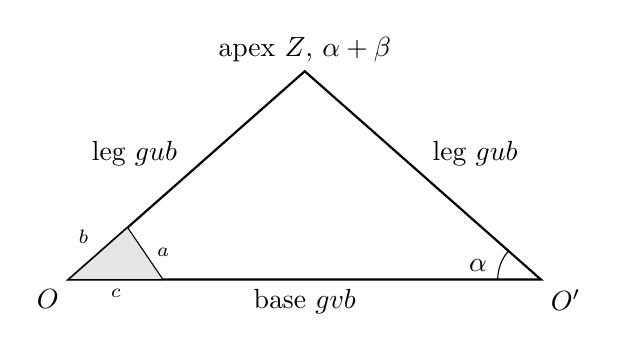
\begin{tikzpicture}[scale=0.5]
  \coordinate (A) at (0,0);
  \coordinate (B) at (12,0);
  \coordinate (C) at (6,5.2915);
  \draw[thick] (A) -- (B) -- (C) -- cycle;
  \node[below left] at (A) {$O$};
  \node[below right] at (B) {$O'$};
  \node[above] at (C) {apex $Z$, $\alpha+\beta$};
  \node[below] at (6,0) {base $gvb$};
  \node[above left] at (3,2.65) {leg $gub$};
  \node[above right] at (9,2.65) {leg $gub$};
  \draw (1.1,0) arc (0:41.41:1.1); \node at (1.6,0.35) {$\alpha$};
  \draw (10.9,0) arc (180:138.59:1.1); \node at (10.4,0.35) {$\alpha$};
  \coordinate (P1) at (2.4,0);
  \coordinate (P2) at ({2.0*0.75},{2.0*0.6614});
  \draw[fill=gray!20] (A) -- (P1) -- (P2) -- cycle;
  \node[below] at (1.2,0) {\scriptsize $c$};
  \node[above left] at (0.75,0.66) {\scriptsize $b$};
  \node[right] at (2.0,0.7) {\scriptsize $a$};
\end{tikzpicture}
\caption{The target $\Omega_{g}$ for $(u,v)=(2,3)$ (not to scale in the number of tiles): base angles $\alpha$, apex $\alpha+\beta$. The corner tile at $O$ (shaded) shows $\alpha$, hence has its edges $b$ and $c$ on the two sides, in one of two orders.}\label{fig:Tg}
\end{figure}

\subsection{The fan lemma and the sector facts}\label{sub:fan}
\begin{lemma}[Fan lemma; \sF]\label{lem:fan}
{\small\noindent\emph{Lean:} \lean{ThmDHalfFan.halfplane_junction_fan}, \lean{APrimeSeat1.straight_vertex}\par}
$k_\alpha\alpha+k_\beta\beta+k_\gamma\gamma=\pi$ with $k_\alpha,k_\beta,k_\gamma\in\N$ if and only if $(k_\alpha,k_\beta,k_\gamma)\in\{(3,1,0),(1,1,1)\}$.
\end{lemma}
\begin{proof}
$\cos\alpha=v/2u$ is rational and lies in $(\tfrac12,1)$, so $\alpha\notin\Q\pi$ (Niven). Now
$k_\alpha\alpha+k_\beta\beta+k_\gamma\gamma=(k_\alpha-3k_\beta+2k_\gamma)\alpha+k_\beta\pi$, which equals $\pi$ only if $k_\beta=1$ and $k_\alpha+2k_\gamma=3$.
\end{proof}
The same computation fills any sector. A sector bounded by two rays from a point $P$ with vertex tiles only (no tile has $P$ interior to an edge) is filled by tiles showing $k_\alpha,k_\beta,k_\gamma$ angles with total the sector angle. This gives the \emph{sector facts}:
\begin{itemize}
\item[\textup{(SF1)}] a sector of angle $\alpha$ is one tile showing $\alpha$; of angle $\beta$, one tile showing $\beta$; of angle $\gamma$, one tile showing $\gamma$ or two showing $\alpha$; of angle $\pi-\gamma=\alpha+\beta$, one $\alpha$-tile and one $\beta$-tile (no $\gamma$); of angle $\pi-\beta-\gamma=\alpha$, one $\alpha$-tile;
\item[\textup{(SF2)}] at a point of a side of $\Omega_{g}$ other than a vertex, the tiles with a vertex there show exactly one $\beta$ and at most one $\gamma$; the same holds for the tiles on one side of a line through an interior point (a half-plane);
\item[\textup{(SF3)}] a base corner carries one tile, showing $\alpha$; the apex carries one $\alpha$-tile and one $\beta$-tile (different tiles, as no tile has angle $\alpha+\beta$); no tile shows $\gamma$ at a vertex of $\Omega_{g}$.
\end{itemize}
(Each is the equation $(k_\alpha-3k_\beta+2k_\gamma)\alpha+k_\beta\pi=\theta$ for the angle $\theta$ of the sector, solved with $\alpha\notin\Q\pi$; for $\theta=\beta=\pi-3\alpha$ it reads $k_\beta=1$, $k_\alpha+2k_\gamma=0$.) Their Lean forms are in \texttt{ThmDHalfFan}, \texttt{ThmDNoGamma}, \texttt{APrimeSeat1}.

\subsection{The two rigidity windows}
\begin{lemma}[Rigidity; \sF]\label{lem:rigid}
{\small\noindent\emph{Lean:} \lean{ThmCRigidity.rel_param}, \lean{ra_int}, \lean{rb_int}, \lean{rc_int_w}\par}
The integer triples $(x,y,z)$ with $xa+yb+zc=0$ are $(y'u+vs,\;uy',\;-us-y'v)$ with $y',s\in\Z$. Consequently, for a segment of length $na$, $nb$ or $nc$ cut into edges $a,b,c$:
\begin{itemize}
\item[\textup{(RA)}] $na$ is cut into $n$ edges $a$ if $n\le v-1$;
\item[\textup{(RB)}] $nb$ is cut into $n$ edges $b$ if $n\le u-1$;
\item[\textup{(RC$_v$)}] $nc$ contains no edge $b$ if $n\le v-1$.
\end{itemize}
The bounds are attained: $va=uc$, $ub=d(a+c)$, $vc=u(a+b)$.
\end{lemma}
\begin{proof}
From $xu^2+y(v^2-u^2)+zuv=0$ and $\gcd(u,v^2-u^2)=1$ we get $u\mid y$; write $y=uy'$ and divide by $u$: $u(x-y'u)=-v(y'v+z)$, so $x-y'u=vs$ and $z=-us-y'v$. A cut of a segment into $x'$ edges $a$, $y$ edges $b$, $z'$ edges $c$ is a relation $(x'-n\delta_a,\,y-n\delta_b,\,z'-n\delta_c)$ with $x',y,z'\ge0$.
\emph{(RA).} Here $x'-n=y'u+vs$, $y=uy'$, $z'=-us-y'v$, so $y'\ge0$. If $y'=0$ and $s\ne0$, then $z'\ge0$ forces $s\le-1$ and $n=x'-vs\ge v$. If $y'\ge1$, then $us\le-y'v$, so $s\le-y'-1$ and $n=x'-y'u-vs\ge v(y'+1)-y'u>v$.
\emph{(RB).} Here $y=n+uy'$, $x'=y'u+vs$, $z'=-us-y'v$. If $n\le u-1$ then $y\ge0$ forces $y'\ge0$. If $y'\ge1$, then $x'\ge0$ and $z'\ge0$ give $-y'u/v\le s\le-y'v/u$, impossible since $u<v$. So $y'=0$, hence $s=0$ and the cut is pure.
\emph{(RC$_v$).} Here $z'=n-us-y'v$, $y=uy'$, $x'=y'u+vs$. Suppose $y\ge1$, so $y'\ge1$. From $x'\ge0$, $s\ge-\lfloor y'u/v\rfloor\ge-(y'-1)$. From $z'\ge0$, $n\ge us+y'v\ge y'v-u(y'-1)=y'd+u\ge d+u=v$.
The bounds are attained by $s=-1,y'=0$ ($va=uc$), $y'=-1,s=1$ ($ub=d(a+c)$) and $y'=1,s=0$ ($vc=u(a+b)$).
\end{proof}
The numbers $v$ (for RA, RC$_v$) and $u$ (for RB) are the \emph{windows}. In the setting of Beeson and Ro\c{s}u (Lemma~BR-30) one number $k$ serves for all three statements; here they split.

\begin{lemma}[Side words; \sF]\label{lem:words}
{\small\noindent\emph{Lean:} \lean{ThmCWords}, \lean{ThmDWords}\par}
If a leg of $\Omega_{g}$ is cut into $n_a$ edges $a$, $n_b$ edges $b$ and $n_c$ edges $c$, then $(n_a,n_b,n_c)=(md+jv,\;u(g-m),\;md-ju)$ with $0\le m\le g$, $j\in\Z$, $md+jv\ge0$ and $md-ju\ge0$. If the base is cut so, then $(n_a,n_b,n_c)=(\bar md+jv,\;gv-\bar mu,\;\bar md-ju)$ with $0\le\bar m\le\lfloor gv/u\rfloor$ and the same inequalities on $j$.
\end{lemma}
\begin{proof}
Lemma~\ref{lem:rigid} applied to the relation $(n_a,n_b-gu,n_c)$, respectively $(n_a,n_b-gv,n_c)$, with $s=m+j$, respectively $s=\bar m+j$.
\end{proof}

\subsection{The quadratic patch}\label{sub:patch}
Let $U$ be a point of a side $\Sigma$ of $\Omega_{g}$ and $\mathsf t_1$ a tile showing $\alpha$ at $U$, with its edge $c$ on $\Sigma$ and its edge $b$ on a ray $UW$ into the triangle. Put $x(i,j)=U+ic\,\hat\imath+jb\,\hat\jmath$ with $\hat\imath$ along $\Sigma$ and $\hat\jmath$ along $UW$ (west, east, north: $-\hat\imath$, $+\hat\imath$, $+\hat\jmath$). Let $\Delta_{i,j}$ be the translate of $\mathsf t_1$ with vertices $x(i,j)$, $x(i+1,j)$, $x(i,j+1)$ (angles $\alpha,\beta,\gamma$), and $\nabla_{i,j}$ its image under the half-turn about the midpoint of its edge $a$, with vertices $x(i+1,j)$, $x(i,j+1)$, $x(i+1,j+1)$ (angles $\gamma,\beta,\alpha$); its edge $c$ is $x(i,j+1)x(i+1,j+1)$ and its edge $b$ is $x(i+1,j)x(i+1,j+1)$. For $1\le r\le s$ let $\mathcal Q(s,r)$ be the set of the $\Delta_{i,j}$ ($j<r$, $i+j\le s-1$) and $\nabla_{i,j}$ ($j<r$, $i+j\le s-2$); it tiles the trapezoid $U\,x(s,0)\,x(s-r,r)\,x(0,r)$. It \emph{occurs} if all its members are tiles of the tiling. Let $\ell_r$ be the line through $x(0,r)$ parallel to $\Sigma$ and $H(w)$ the statement that $\mathcal Q(w,w)$ occurs. For a $c$-block $\mathsf t_1,\dots,\mathsf t_n$ from $U$, $\mathsf t_{i+1}=\Delta_{i,0}$ iff $\mathsf t_{i+1}$ shows $\alpha$ at its west end. Figure~\ref{fig:patch} shows $\mathcal Q(3,3)$.

\begin{figure}[ht]
\centering
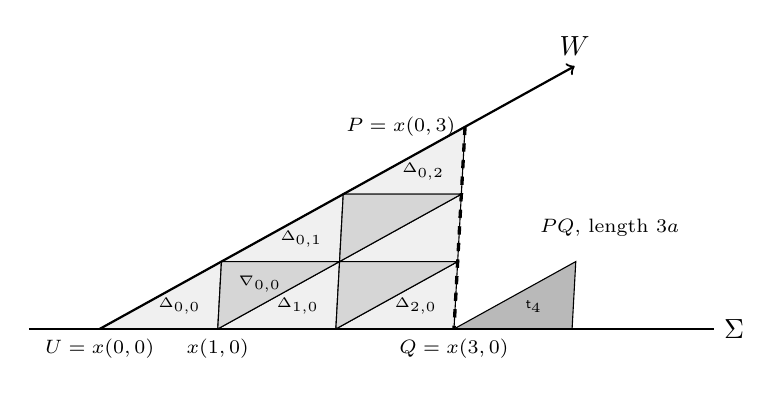
\begin{tikzpicture}[scale=1.5]
  % schematic lattice, see \XX
  \foreach \j in {0,1,2}{\foreach \i in {0,1,2}{\ifnum\numexpr\i+\j\relax<3
     \draw[fill=gray!12] \XX{\i}{\j} -- \XX{\i+1}{\j} -- \XX{\i}{\j+1} -- cycle;\fi}}
  \foreach \j in {0,1}{\foreach \i in {0,1}{\ifnum\numexpr\i+\j\relax<2
     \draw[fill=gray!32] \XX{\i+1}{\j} -- \XX{\i}{\j+1} -- \XX{\i+1}{\j+1} -- cycle;\fi}}
  \draw[fill=gray!55] \XX{3}{0} -- \XX{4}{0} -- \XX{3}{1} -- cycle;
  \draw[thick] (-0.6,0) -- (5.2,0) node[right] {$\Sigma$};
  \draw[thick,->] (0,0) -- ({1.03125*3.9},{0.57057*3.9}) node[above] {$W$};
  \draw[very thick,dashed] \XX{0}{3} -- \XX{3}{0};
  \node[below] at (0,0) {\scriptsize $U=x(0,0)$};
  \node[below] at (1,0) {\scriptsize $x(1,0)$};
  \node[below] at (3,0) {\scriptsize $Q=x(3,0)$};
  \node[left] at \XX{0}{3} {\scriptsize $P=x(0,3)$};
  \node at \XX{1/3}{1/3} {\tiny $\Delta_{0,0}$};
  \node at \XX{2/3}{2/3} {\tiny $\nabla_{0,0}$};
  \node at \XX{4/3}{1/3} {\tiny $\Delta_{1,0}$};
  \node at \XX{7/3}{1/3} {\tiny $\Delta_{2,0}$};
  \node at \XX{1/3}{4/3} {\tiny $\Delta_{0,1}$};
  \node at \XX{1/3}{7/3} {\tiny $\Delta_{0,2}$};
  \node at \XX{10/3}{1/3} {\tiny $\mathsf t_4$};
  \node[right] at \XX{2.1}{1.5} {\scriptsize $PQ$, length $3a$};
\end{tikzpicture}
\caption{The quadratic patch $\mathcal Q(3,3)$, stage $H(3)$, on a block of $n\ge4$ edges $c$ (to scale in the angles: the lattice is drawn for $(u,v)=(4,7)$, where $a=16$, $b=33$, $c=28$, $\cos\alpha=7/8$ and $\alpha=28.96^\circ$, $\beta=93.1^\circ$, $\gamma=57.9^\circ$). Light: $\Delta_{i,j}$; medium: $\nabla_{i,j}$; dark: the next tile $\mathsf t_4=\Delta_{3,0}$ of the block. The diagonal $PQ$ is made of the edges $a$ of the three tiles west of it.}\label{fig:patch}
\end{figure}

\subsection{The trapezoid lemma}\label{sub:trap}
\begin{lemma}[Trapezoid lemma; adapted from BR-32; \sF]\label{lem:trap}
{\small\noindent\emph{Lean:} \lean{ThmDL32.lemma32}\par}
Let $\mathsf t_1,\dots,\mathsf t_n$ be a $c$-block on a side $\Sigma$ of $\Omega_{g}$ from $U$, $n\le v-1$, stopped at its far end $V$. Let $1\le r<s\le n$. Then the following cannot both hold: \textup{(i)} $\mathcal Q(s,r)$ occurs; \textup{(ii)} for some $i_0$ with $0\le i_0<s-r$ a tile north of $\ell_r$ has a vertex at $x(i_0,r)$ and its edge $b$ on $\ell_r$ running east from $x(i_0,r)$.
\end{lemma}
\emph{Idea.} At a lattice point $x(s-j,j)$ on the east edge of the patch the remaining sector is $\alpha$; it is filled by one tile with edges $b,c$ along the two rays, so either it continues the patch ($c$ east) or it lays an edge $b$ east along $\ell_j$ (alternative (ii)). In the second case the edge $b$ cannot end at a lattice point (the row below is covered by edges $c$, and (RC$_v$)), so it runs over a lattice point $q_r$, and the tile at $q_r$ forces a column of $\nabla$ tiles that lets the patch grow, against maximality. The claims follow this.
\begin{proof}
Suppose the lemma fails and take $(s,r,i_0)$ with $s$ maximal. Put $q_j=x(s-j,j)$ (so $q_0=x(s,0)$ and $q_r=x(s-r,r)$) and $\sigma=q_0q_r$. The tiles of $\mathcal Q(s,r)$ west of $\sigma$ have the edges $a$ of $\Delta_{s-1-j,j}$ ($0\le j<r$) on $\sigma$, from $q_j$ (showing $\beta$) to $q_{j+1}$ (showing $\gamma$).
\begin{itemize}
\item[\textbf{Tr1}] \emph{The edges on $\ell_r$ of the tiles north of $\ell_r$ cover $[x(0,r),q_r]$ without overlap.} South of $\ell_r$ this segment is the union of the edges $c$ of $\nabla_{i,r-1}$, $0\le i<s-r$, so no tile straddles it.
\item[\textbf{Tr2}] \emph{$q_r$ is interior to an edge $e_\ast$ on $\ell_r$ of a tile north of $\ell_r$.} By (ii) $x(i_0,r)$ is a vertex of one of these tiles, followed by an edge $b$. If $q_r$ were also a vertex of one, the edges between $x(i_0,r)$ and $q_r$ would cut $(s-r-i_0)c$ into edges including a $b$; but $1\le s-r-i_0\le s-1\le v-2$, against (RC$_v$).
\item[\textbf{Tr3}] \emph{$q_r$ is an interior point of $\Omega_{g}$.} The edge $e_\ast$ lies in $\Omega_{g}$ and has $q_r$ in its relative interior. If $q_r$ were on a side of $\Omega_{g}$, a segment of $\Omega_{g}$ through $q_r$ with $q_r$ in its interior would lie on that side, so $\ell_r$ would be a side line. But $\ell_r$ is parallel to $\Sigma$ at positive distance (since $r\ge1$), and no two sides of a triangle are parallel.
\item[\textbf{Tr4}] \emph{The sector east of $\sigma$ at $q_r$ is one tile $t_\ast$ showing $\beta$ at $q_r$, with an edge on $\sigma$.} Around $q_r$ the tile of $e_\ast$ contributes $\pi$ (north), and south $\nabla_{s-r-1,r-1}$ and $\Delta_{s-r,r-1}$ show $\alpha$ and $\gamma$ and fill the sector between west $\ell_r$ and $\sigma$. The rest is $2\pi-\pi-\alpha-\gamma=\beta$; use (SF1).
\item[\textbf{Tr5}] \emph{$s<n$.} Suppose $s=n$, so $q_0=V$, and $\mathsf t_n=\Delta_{n-1,0}$ shows $\beta$ at $V$. (a) If $V$ is not a vertex of $\Omega_{g}$, the block is stopped there: the tile east of $V$ on $\Sigma$ shows $\gamma$ at $V$, and the angles at $V$ add up to $\pi$, so the sector between that tile and $\sigma$ is $\pi-\beta-\gamma=\alpha$. (b) If $V$ is a vertex it is not a base corner (a base corner carries one tile, showing $\alpha$, while $\mathsf t_n$ shows $\beta$ at $V$), so it is the apex, of angle $\alpha+\beta$; $\mathsf t_n$ takes $\beta$ and the sector left between $\sigma$ and the other leg is $\alpha$. In both cases the sector east of $\sigma$ at $V$ is filled by one $\alpha$-tile $\mathsf t'$ (SF1), whose edges at $V$ are $b$ and $c$, so one of them lies on $\sigma$.
\emph{The segment $\sigma$ is clamped at both ends.} At $q_0=V\in\partial\Omega$ the line of $\sigma$ contains the interior point $q_r$ (Tr3), so it is not a side line, and Lemma~\ref{lem:clamp}(iii) applies; it covers $V$ on a side and $V$ the apex alike (an edge on that line with $V$ in its relative interior would leave $\Omega$ beyond $V$). At $q_r$: a tile east of $\sigma$ with an edge on the line of $\sigma$ containing $q_r$ in its relative interior would contain the half-disc east of that line, which meets the tile of $e_\ast$ (Tr2) in an open set. The open segment $(q_0,q_r)$ lies in the interior of $\Omega$ (an interior point and a boundary point of a convex set, not on a side line) and contains no interior point of a tile, because west of $\sigma$ the edges $a$ of the tiles of $\mathcal Q(s,r)$ cover it. By Lemma~\ref{lem:partition} the edges on $\sigma$ of the tiles east of $\sigma$ cut $\sigma$, of length $ra$; as $r<s=n\le v-1$, (RA) says they are all edges $a$, whereas $\mathsf t'$ has an edge $b$ or $c$ on $\sigma$. This is a contradiction.
\item[\textbf{Tr6}] \emph{The tiles east of $\sigma$ lay $r$ edges $a$ on $\sigma$, with endpoints $q_0,\dots,q_r$.} West of $\sigma$ the edges $a$ of the patch lie on it, so no tile straddles $\sigma$. The segment is clamped at $q_r$: an east tile with an edge on the line of $\sigma$ through $q_r$ in its relative interior would contain the half-disc east of that line, which meets the tile of $e_\ast$ (Tr2). It is clamped at $q_0$: $q_0$ is on $\Sigma$, and such a tile would cross $\Sigma$ out of $\Omega_{g}$. By Lemma~\ref{lem:partition} the edges cut $\sigma$, of length $ra$ with $r<v$; by (RA) they are $r$ edges $a$.
\item[\textbf{Tr7}] \emph{The column.} The top edge is the edge $a$ of $t_\ast$, with $\beta$ at $q_r$ (Tr4), hence $\gamma$ at $q_{r-1}$. At each $q_j$, $0<j<r$, the east tiles fill a half-plane, so by (SF2) at most one shows $\gamma$; by downward induction the tile on $q_jq_{j+1}$ shows $\gamma$ at $q_j$ and $\beta$ at $q_{j+1}$. A tile on the east side of a segment of length $a$ with these end angles is unique (the third vertex is determined), so it is the half-turn image of $\Delta_{s-1-j,j}$: it is $\nabla_{s-1-j,j}$. In particular $\nabla_{s-1,0}$ shows $\gamma$ at $q_0$.
\item[\textbf{Tr8}] $\mathsf t_{s+1}=\Delta_{s,0}$. Since $s<n$, $\mathsf t_{s+1}$ exists. At $q_0$ north of $\Sigma$, $\mathsf t_s=\Delta_{s-1,0}$ and $\nabla_{s-1,0}$ show $\beta$ and $\gamma$, leaving a sector $\alpha$; so $\mathsf t_{s+1}$ shows $\alpha$ at $q_0$.
\item[\textbf{Tr9}] \emph{The five-tile fan} (Figure~\ref{fig:fan}). For $1\le j\le r-1$ the tiles $\Delta_{s-j-1,j}$, $\Delta_{s-j,j-1}$, $\nabla_{s-j-1,j-1}$ (in $\mathcal Q(s,r)$) and $\nabla_{s-j-1,j}$, $\nabla_{s-j,j-1}$ (in the column of Tr7) show $\beta,\gamma,\alpha,\gamma,\beta$ at $x(s-j,j)$. They leave a sector $\alpha$ between the edge $b$ of $\nabla_{s-j-1,j}$ (direction $\hat\jmath$) and the edge $c$ of $\nabla_{s-j,j-1}$ (along $\ell_j$, east). It is one tile $\mathsf t^\ast_j$ showing $\alpha$ there (SF1), whose edges $b,c$ lie on these two rays: either $\mathsf t^\ast_j=\Delta_{s-j,j}$ ($c$ east, $b$ north), or $\mathsf t^\ast_j$ has its edge $b$ on $\ell_j$ running east.
\item[\textbf{Tr10}] \emph{Contradiction with maximality.} If $\mathsf t^\ast_j=\Delta_{s-j,j}$ for all $1\le j\le r-1$, then $\mathcal Q(s+1,r)$ occurs (Tr7, Tr8, Tr9) and (ii) holds for $(s+1,r)$ with the same $i_0<s-r<s+1-r$. Otherwise let $j^*$ be least with $\mathsf t^\ast_{j^*}\ne\Delta_{s-j^*,j^*}$: $\mathcal Q(s+1,j^*)$ occurs and $\mathsf t^\ast_{j^*}$ witnesses (ii) for $(s+1,j^*)$ with $i_0=s-j^*<s+1-j^*$. As $s+1\le n$, either contradicts the maximality of $s$.
\end{itemize}
\end{proof}
The rigidity used is (RC$_v$) in Tr2 and (RA) in Tr5, Tr6, both with window $v$, for $n\le v-1$; neither RB nor an angle inequality occurs (the only angle fact is (SF2), the Fan lemma). The clamp of Tr6 at $q_r$ is the reason Tr2 asks for $q_r$ to be \emph{interior} to an edge.

\begin{figure}[ht]
\centering
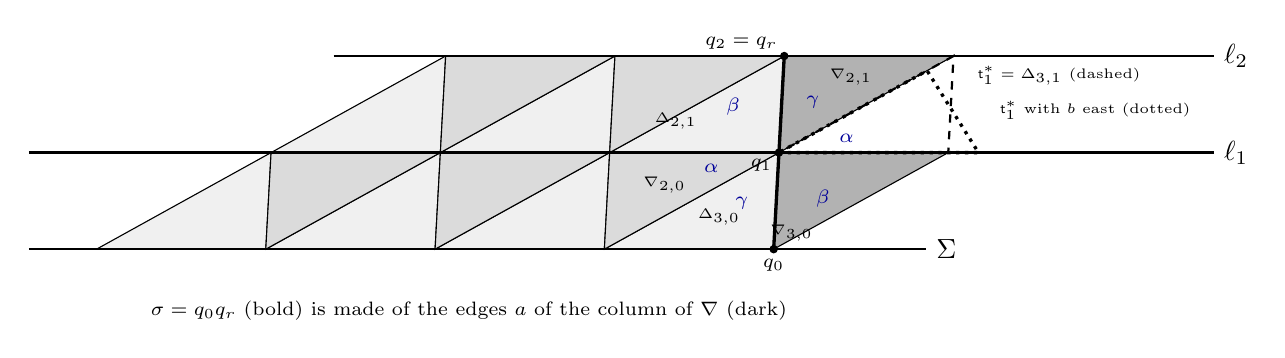
\begin{tikzpicture}[scale=2.15]
  % schematic lattice, s=4, r=2: Q(4,2) light; column nabla_{3,0}, nabla_{2,1} dark
  \foreach \j in {0,1}{\foreach \i in {0,1,2,3}{\ifnum\numexpr\i+\j\relax<4
     \draw[fill=gray!12] \XX{\i}{\j} -- \XX{\i+1}{\j} -- \XX{\i}{\j+1} -- cycle;\fi}}
  \foreach \j in {0,1}{\foreach \i in {0,1,2}{\ifnum\numexpr\i+\j\relax<3
     \draw[fill=gray!28] \XX{\i+1}{\j} -- \XX{\i}{\j+1} -- \XX{\i+1}{\j+1} -- cycle;\fi}}
  % the column of nablas outside Q(4,2): nabla_{3,0}, nabla_{2,1}
  \draw[fill=gray!60] \XX{4}{0} -- \XX{3}{1} -- \XX{4}{1} -- cycle;
  \draw[fill=gray!60] \XX{3}{1} -- \XX{2}{2} -- \XX{3}{2} -- cycle;
  % the two alternatives for \mathsf t^\ast_1 at q_1 = x(3,1)
  \draw[dashed,thick] \XX{3}{1} -- \XX{4}{1} -- \XX{3}{2} -- cycle;
  \draw[dotted,very thick] \XX{3}{1} -- ({4.03125+1.17857},0.57057) -- ({4.03125+0.875},{0.57057+0.48412}) -- cycle;
  \draw[thick] (-0.4,0) -- (4.9,0) node[right] {$\Sigma$};
  \draw[thick] (-0.4,0.57057) -- (6.6,0.57057) node[right] {$\ell_1$};
  \draw[thick] (1.4,1.14114) -- (6.6,1.14114) node[right] {$\ell_2$};
  \draw[very thick] \XX{4}{0} -- \XX{2}{2};
  \fill \XX{4}{0} circle (0.025) node[below] {\scriptsize $q_0$};
  \fill \XX{3}{1} circle (0.025) node[below left=-1pt] {\scriptsize $q_1$};
  \fill \XX{2}{2} circle (0.025) node[above left=-1pt] {\scriptsize $q_2=q_r$};
  % angles at q_1 = x(3,1), radius 0.33: beta (Delta_{2,1}), alpha (nabla_{2,0}), gamma (Delta_{3,0}), beta (nabla_{3,0}), gamma (nabla_{2,1}), alpha (t*_1)
  \node[blue!60!black] at ({4.03125-0.27},{0.57057+0.27}) {\scriptsize $\beta$};
  \node[blue!60!black] at ({4.03125-0.40},{0.57057-0.09}) {\scriptsize $\alpha$};
  \node[blue!60!black] at ({4.03125-0.22},{0.57057-0.30}) {\scriptsize $\gamma$};
  \node[blue!60!black] at ({4.03125+0.26},{0.57057-0.27}) {\scriptsize $\beta$};
  \node[blue!60!black] at ({4.03125+0.20},{0.57057+0.30}) {\scriptsize $\gamma$};
  \node[blue!60!black] at ({4.03125+0.40},{0.57057+0.085}) {\scriptsize $\alpha$};
  \node at \XX{2+0.05}{1+0.33} {\tiny $\Delta_{2,1}$};
  \node at \XX{3+1/3}{1/3} {\tiny $\Delta_{3,0}$};
  \node at \XX{2+2/3}{2/3} {\tiny $\nabla_{2,0}$};
  \node at \XX{3.93}{0.17} {\tiny $\nabla_{3,0}$};
  \node at \XX{2.62}{1.78} {\tiny $\nabla_{2,1}$};
  \node[above right] at \XX{3.5}{1.6} {\tiny $\mathsf t^\ast_1=\Delta_{3,1}$ (dashed)};
  \node[right] at ({4.03125+1.25},{0.57057+0.25}) {\tiny $\mathsf t^\ast_1$ with $b$ east (dotted)};
  \node[below] at (2.2,-0.25) {\scriptsize $\sigma=q_0q_r$ (bold) is made of the edges $a$ of the column of $\nabla$ (dark)};
\end{tikzpicture}
\caption{The five-tile fan of Tr9 for $(u,v)=(4,7)$, $s=4$, $r=2$, $j=1$ (angles to scale, as in Figure~\ref{fig:patch}). Light and medium: $\mathcal Q(4,2)$. Dark: the column $\nabla_{3,0},\nabla_{2,1}$ of Tr7, which lies outside $\mathcal Q(4,2)$ and supplies two of the five tiles around $q_1=x(3,1)$; the other three are $\Delta_{2,1},\Delta_{3,0},\nabla_{2,0}$. The angles of the five tiles at $q_1$ ($\beta,\alpha,\gamma,\beta,\gamma$, in blue) add up to $2\pi-\alpha$, so that the angle $\alpha$ is left to be filled (angles to scale: $93.1^\circ+29.0^\circ+57.9^\circ+93.1^\circ+57.9^\circ=331.0^\circ$, remaining $29.0^\circ$). The remaining sector at $q_1$ is filled by a tile $\mathsf t^\ast_1$: dashed, the lattice tile $\Delta_{3,1}$; dotted, the alternative with its edge $b$ east along $\ell_1$.}\label{fig:fan}
\end{figure}

\subsection{The row lemma: interior starts and corner starts}\label{sub:rows}
\begin{lemma}[Row lemma; \sF]\label{lem:rows}
{\small\noindent\emph{Lean:} \lean{ThmDInterior.lemma33_interior} for \textup{(I)}; \lean{ThmDK2Final.lemmaK2_final}, \lean{ThmDGeoLegCorner.leg_corner_start} for \textup{(K)}\par}
Let $\mathsf t_1,\dots,\mathsf t_n$ be a $c$-block on a side $\Sigma$ of $\Omega_{g}$ from $U$, $\mathsf t_1$ showing $\alpha$ at $U$ with its edge $b$ on the ray $UW$, stopped at its far end $V$. Assume one of:
\begin{itemize}
\item[\textup{(I)}] (BR-33; $U$ may be the apex.) $n\le u-1$, and some tile with a vertex at $U$, on the other side of $UW$ from $\mathsf t_1$, has an edge $a$ or $c$ on $UW$.
\item[\textup{(K)}] (Lemma~K.) $U$ is a base corner of $\Omega_{g}$, $UW$ is the other side $\Sigma'$ at $U$, $n\le v-1$ and $|\Sigma'|>nb$.
\end{itemize}
Then this is impossible. In particular a $c$-block from a base corner that is stopped at its far end has at least $v$ edges, if $|\Sigma'|>(v-1)b$.
\end{lemma}
(For a run on a leg of $\Omega_{g}$ the other side at the base corner is the base, of length $gvb>vb$ if $g>1$; for a run on the base, $\Sigma'$ is a leg, of length $gub\ge2ub>(v-1)b$ if $g\ge2$.)
\begin{proof}
We show that $H(w)$ implies $w<n$ and $H(w+1)$, for $1\le w\le n$; since $H(1)$ holds ($\mathsf t_1=\Delta_{0,0}$), $H(n)$ would give $n<n$. Assume $H(w)$; put $P=x(0,w)$, $Q=x(w,0)$, $p_i=x(i,w-i)$ ($0\le i\le w$).
\begin{itemize}
\item[\textbf{Rw1}] \emph{The line $UP$ is a wall beyond $P$.} \emph{Case (K):} $UP\subset\Sigma'$, a side of $\Omega_{g}$, and $P$ is interior to $\Sigma'$ because $|UP|=wb\le nb<|\Sigma'|$; beyond $P$ the wall is $\Sigma'$ itself. Nothing is used about rigidity. \emph{Case (I):} the tiles west of $UP$ have edges on $UP$ starting at $U$, the first being the edge $a$ or $c$ of the given tile. The open segment $(U,P)$ lies in the interior of $\Omega$: $P$ is a vertex of the tile $\Delta_{0,w-1}$, so $P\in\Omega$; if $U$ is interior to $\Omega$ this is clear; if $U\in\partial\Omega$ (a point of a leg, or the apex), the ray $UW$ is not a side line, because it makes the angle $\alpha$ with the side $\Sigma$ at $U$, which is smaller than the angle of $\Omega$ at $U$ (it is $\pi$ at a point of a side and $\alpha+\beta$ at the apex), and by convexity the open segment is interior (Lemma~\ref{lem:clamp}(iii) and its proof). This is the written counterpart of the Lean hypotheses \lean{hch} and \lean{hwedge} (Appendix~\ref{app:lean}, rows 2 and 8). If $P$ were a vertex of a west tile or a point of the boundary of $\Omega_{g}$, the edges on $UP$ of the west tiles, which start at $U$ with an $a$ or a $c$, would cut $wb$ (Lemma~\ref{lem:partition}); but $w\le n\le u-1$, against (RB). So $P$ is interior to an edge of a west tile and $UP$ continues as a tile edge beyond $P$.
\item[\textbf{Rw2}] \emph{The sector at $P$.} East of $UP$ lie the edges $b$ of $\Delta_{0,j}$; $\Delta_{0,w-1}$ shows $\gamma$ at $P$. The sector between $PQ$ and the continuation of $UP$ is $\pi-\gamma=\alpha+\beta$: one $\alpha$-tile and one $\beta$-tile, none showing $\gamma$ (SF1).
\item[\textbf{Rw3}] \emph{$w<n$.} Suppose $w=n$, so $Q=V$ and $\mathsf t_n$ shows $\beta$ at $V$. (a) $V$ is not a vertex of $\Omega_{g}$: the block is stopped at $V$, so the tile east of $V$ on $\Sigma$ shows $\gamma$ and the sector between it and $PQ$ is $\pi-\beta-\gamma=\alpha$. (b) $V$ is the apex: $\mathsf t_n$ takes the $\beta$ of the apex angle $\alpha+\beta$ and the sector left between $PQ$ and the other leg is $\alpha$. (c) $V$ is a base corner: impossible, as the corner carries one tile showing $\alpha$. In (a), (b) one $\alpha$-tile fills the sector, and its edge on $PQ$ is $b$ or $c$ (the edges at $\alpha$ are $b,c$). The segment $PQ$ is clamped at $P$ (the wall of Rw1: in case (I) an east tile with an edge on the line $PQ$ containing $P$ in its relative interior would contain the continuation of $UP$ in its interior; in case (K) it would leave $\Omega$ across $\Sigma'$, Lemma~\ref{lem:clamp}(iii)) and at $Q$ ($Q\in\partial\Omega$ and the line $PQ$ meets the interior of $\Omega$, so it is not a side line: Lemma~\ref{lem:clamp}(iii), which covers $Q$ on a side and $Q$ the apex alike). The open segment lies in the interior of $\Omega$ and contains no interior point of a tile, since the edges $a$ of the $w$ tiles of $\mathcal Q(w,w)$ west of it cover it. So by Lemma~\ref{lem:partition} the east edges cut $PQ$, of length $wa$ with $w<v$, and one of them is $b$ or $c$; this contradicts (RA).
\item[\textbf{Rw4}] \emph{$PQ$ is cut into $w$ edges $a$, a row of $\nabla$.} For $w<n$ the same clamps and (RA) give $w$ edges $a$ with endpoints $p_0,\dots,p_w$. No east tile shows $\gamma$ at $p_0=P$ (Rw2); at each interior $p_i$ the east tiles fill a half-plane, so at most one shows $\gamma$ (SF2). By induction on $i$, the tile on $p_ip_{i+1}$ shows $\beta$ at $p_i$ and $\gamma$ at $p_{i+1}$, so it is $\nabla_{i,w-1-i}$ (uniqueness as in Tr7). In particular $\nabla_{w-1,0}$ shows $\gamma$ at $Q$.
\item[\textbf{Rw5}] \emph{$H(w+1)$.} At $Q$ north of $\Sigma$, $\mathsf t_w=\Delta_{w-1,0}$ and $\nabla_{w-1,0}$ show $\beta+\gamma$, so $\mathsf t_{w+1}=\Delta_{w,0}$. For $1\le j\le w-1$ the five-tile fan of Tr9 (with $s=w$) leaves an $\alpha$-sector at $x(w-j,j)$; at $P$ the tiles $\Delta_{0,w-1}$ and $\nabla_{0,w-1}$ show $\gamma+\beta$ and leave an $\alpha$-sector between the continuation of $UP$ and the edge $c$ of $\nabla_{0,w-1}$. So for $1\le j\le w$ there is a tile $\mathsf t^\ast_j$ showing $\alpha$ at $x(w-j,j)$, with $\mathsf t^\ast_j=\Delta_{w-j,j}$ or $\mathsf t^\ast_j$ having its edge $b$ on $\ell_j$ running east. If all $\mathsf t^\ast_j=\Delta_{w-j,j}$, then $H(w+1)$ holds. Otherwise, for the least $j^*$ with $\mathsf t^\ast_{j^*}\ne\Delta$, $\mathcal Q(w+1,j^*)$ occurs and $\mathsf t^\ast_{j^*}$ satisfies (ii) of Lemma~\ref{lem:trap} with $s=w+1$, $r=j^*$, $i_0=w-j^*$; since $1\le j^*\le w<w+1\le n\le v-1$, Lemma~\ref{lem:trap} gives a contradiction.
\end{itemize}
\emph{Windows.} Case (K): (RA) in Rw3, Rw4 and in Lemma~\ref{lem:trap}; (RC$_v$) in Lemma~\ref{lem:trap}; all with arguments $\le n\le v-1$; RB is not used. Case (I): additionally (RB) for $wb$ in Rw1, $w\le n\le u-1$.
\end{proof}

\paragraph{Lemma K in full: the proof of case (K).} The proof of Lemma~\ref{lem:rows} above covers both cases; here is case (K) alone, with every use of the corner written out, so that the difference from BR-33 and BR-34 can be checked line by line. Let $O$ be a base corner of $\Omega_{\bar g}$, $\Sigma,\Sigma'$ the sides at $O$, and $\mathsf t_1,\dots,\mathsf t_n$ a $c$-block on $\Sigma$ from $O$ (so $\mathsf t_1$ shows $\alpha$ at $O$), stopped at its far end $V$, with $n\le v-1$ and $|\Sigma'|>nb$. Put $U=O$.
\begin{itemize}
\item[\textbf{Cr0}] \emph{Which hypothesis of BR-34 fails.} BR-34 asks for a second tile with a vertex at $U$, on the other side of the ray along the edge $b$ of $\mathsf t_1$, with an edge $a$ or $c$ on that ray; BR-33 then excludes the short stopped run, and uses the second tile to know that the ray is a wall beyond $P=x(0,w)$ (the first step of their induction from $H(w)$ to $H(w+1)$). At $O$ the angle of $\Omega$ is $\alpha$, so by (SF3) $\mathsf t_1$ is the only tile with a vertex at $O$, its edges $c$ and $b$ lie on $\Sigma$ and $\Sigma'$, and the other side of $\Sigma'$ is outside $\Omega$. The hypothesis fails, and nothing else in the induction needs the second tile.
\item[\textbf{Cr1}] \emph{The target side is the wall.} The ray $UW$ is $\Sigma'$ (the edge $b$ of $\mathsf t_1$ lies on $\Sigma'$), and $x(0,w)=U+wb\,\hat\jmath\in\Sigma'$. For $1\le w\le n$ we have $|UP|=wb\le nb<|\Sigma'|$, so $P$ is in the relative interior of the side $\Sigma'$. The points of $\Sigma'$ beyond $P$ are in $\partial\Omega$, hence interior to no tile (the interior of a tile lies in $\operatorname{int}\Omega$), so $\Sigma'$ is a wall beyond $P$ in the sense of Section~\ref{sub:runsetting}. This is the only place where $|\Sigma'|>nb$ is used, and no rigidity (RB) is involved. Two consequences: \textup{(W1)} the tiles with a vertex at $P$ lie in the closed half-plane of $\Sigma'$ that contains $\Omega$, and their angles add up to $\pi$ (Proposition~\ref{prop:basics}(ii)); \textup{(W2)} a segment $[P,Q']$ with $Q'\in\Omega\setminus\Sigma'$ is clamped at $P$, by Lemma~\ref{lem:clamp}(iii).
\item[\textbf{Cr2}] \emph{Induction.} $H(1)$ holds since $\mathsf t_1=\Delta_{0,0}$. We show: if $1\le w\le n$ and $H(w)$, then $w<n$ and $H(w+1)$. Then $H(n)$ would give $n<n$, so the block does not exist. Put $P=x(0,w)$, $Q=x(w,0)$, $p_i=x(i,w-i)$.
\item[\textbf{Cr3}] \emph{The sector at $P$.} $\Delta_{0,w-1}\in\mathcal Q(w,w)$ has its edge $b$ on $\Sigma'$ and shows $\gamma$ at $P$, with its edge $a$ on $PQ$. By (W1) the remaining sector at $P$, between $PQ$ and the part of $\Sigma'$ beyond $P$, has the angle $\pi-\gamma=\alpha+\beta$; by (SF1) it is one $\alpha$-tile and one $\beta$-tile, and no tile shows $\gamma$ at $P$ east of $PQ$.
\item[\textbf{Cr4}] \emph{$PQ$ is clamped and cut into edges $a$.} $P\in\Sigma'$ and $Q\in\Sigma$ with $\Sigma\ne\Sigma'$, so $(P,Q)$ lies in the interior of $\Omega$; west of $PQ$ it is covered by the edges $a$ of the $w$ tiles of $\mathcal Q(w,w)$, so it contains no interior point of a tile. It is clamped at $P$ by (W2) and at $Q\in\partial\Omega$ by Lemma~\ref{lem:clamp}(iii) (the line $PQ$ meets the interior of $\Omega$). By Lemma~\ref{lem:partition} the edges on $PQ$ of the east tiles cut a segment of length $wa$ with $w\le n\le v-1$; by (RA) they are $w$ edges $a$.
\item[\textbf{Cr5}] \emph{$w<n$.} Suppose $w=n$, so $Q=V$ and $\mathsf t_n$ shows $\beta$ at $V$. If $V$ is not a vertex of $\Omega_{\bar g}$, the block is stopped, the tile east of $V$ on $\Sigma$ shows $\gamma$ and the sector between it and $PQ$ is $\pi-\beta-\gamma=\alpha$. If $V$ is the apex, $\mathsf t_n$ takes the $\beta$ of the angle $\alpha+\beta$ and the sector between $PQ$ and the other leg is $\alpha$. $V$ is not the other base corner, by (SF3). In both cases one $\alpha$-tile fills the sector, with an edge $b$ or $c$ on $PQ$; this contradicts Cr4.
\item[\textbf{Cr6}] \emph{The row of $\nabla$ tiles.} For $w<n$ the edges on $PQ$ are $w$ edges $a$ with endpoints $p_0=P,\dots,p_w=Q$. No east tile shows $\gamma$ at $p_0$ (Cr3); at each interior $p_i$ the east tiles fill a half-plane, so at most one shows $\gamma$ (SF2). By induction on $i$ the east tile on $p_ip_{i+1}$ shows $\beta$ at $p_i$ and $\gamma$ at $p_{i+1}$, so it is $\nabla_{i,w-1-i}$ (uniqueness as in Tr7). In particular $\nabla_{w-1,0}$ shows $\gamma$ at $Q$.
\item[\textbf{Cr7}] \emph{$H(w+1)$.} At $Q$ north of $\Sigma$, $\mathsf t_w$ and $\nabla_{w-1,0}$ show $\beta+\gamma$, so $\mathsf t_{w+1}=\Delta_{w,0}$. For $1\le j\le w-1$ the five-tile fan of Tr9 (with $s=w$) leaves an $\alpha$-sector at $x(w-j,j)$; at $P$, $\Delta_{0,w-1}$ and $\nabla_{0,w-1}$ show $\gamma+\beta$ and leave an $\alpha$-sector between $\Sigma'$ beyond $P$ and the edge $c$ of $\nabla_{0,w-1}$. For $1\le j\le w$ it is filled by one tile $\mathsf t^\ast_j$ showing $\alpha$, with edges $b,c$ on the two rays: $\mathsf t^\ast_j=\Delta_{w-j,j}$, or $\mathsf t^\ast_j$ has its edge $b$ on $\ell_j$ running east. If all are lattice tiles, $H(w+1)$ holds. Otherwise, for the least $j^\ast$ with $\mathsf t^\ast_{j^\ast}\ne\Delta_{w-j^\ast,j^\ast}$, $\mathcal Q(w+1,j^\ast)$ occurs and $\mathsf t^\ast_{j^\ast}$ satisfies (ii) of Lemma~\ref{lem:trap} with $s=w+1\le n\le v-1$, $r=j^\ast$, $i_0=w-j^\ast$: a contradiction.
\end{itemize}
Only (RA) and (RC$_v$) occur, for arguments $\le n\le v-1$. \textbf{Lemma K contributes the wall of Cr1}: in case (I) the tile across $UW$ is used \emph{only} to keep $UW$ a wall beyond $P$, at the price of (RB) with the window $u$. As a by-product only windows of size $v$ occur, so the conclusion is $n\ge v$ rather than $n\ge u$. \textbf{Theorem~F uses only $n\ge u$}: what is used is that the hypothesis of BR-34 can be dropped at a base corner. The bound $n\ge v$ is not used anywhere in this paper; it is sharp for this argument, since at $n=v$ the diagonal $va=uc$ has a second decomposition and Cr4 no longer forces $v$ edges $a$.

\begin{remark}
In the $19\,600$-tiling of Section~\ref{sec:herdt} a leg begins at a base corner with a block of $3=u$ edges $c$ followed by an edge $b$; this block is not stopped, so it is not an instance of Lemma~K and does not test it. The unstopped half of Lemma~K (that $\mathcal Q(n,n)$ occurs and $\Sigma'$ begins with $\min(n,v)$ edges $b$) is not proved here and not used.
\end{remark}

\subsection{The counting identity and the apex property}\label{sub:counting}
Let a leg of $\Omega_{g}$ be traversed from one end to the other, and let $\eta_1,\dots,\eta_h$ be the edges of the tiles that lie on it, in order; $h=n_a+n_b+n_c$. At each of the $h-1$ junctions between $\eta_i$ and $\eta_{i+1}$ the tiles with a vertex there have angles summing to $\pi$, so by Lemma~\ref{lem:fan} exactly one angle $\beta$ occurs there. The tile of $\eta_i$ and the tile of $\eta_{i+1}$ are different tiles (two edges of one tile meet at an angle less than $\pi$); write $\kappa_i$ for the number of angles $\beta$ at the junction among all other tiles with a vertex there.
\begin{lemma}[Counting identity; \sF]\label{lem:counting}
{\small\noindent\emph{Lean:} \lean{APrimeSeat1.counting_identity}, \lean{ThmDCount.counting_identity_gen}, \lean{ThmDCount.q_pos_of_ends}\par}
Let $\kappa_\beta=\sum_i\kappa_i$ and let $\varepsilon_{\rm first},\varepsilon_{\rm last}\in\{0,1\}$ be $1$ iff the first edge has its first end marked $\beta$, respectively the last edge its last end. Then $\kappa_\beta=n_b-1+\varepsilon_{\rm first}+\varepsilon_{\rm last}$. In particular a leg with $\alpha$ at both ends (both ends not marked $\beta$) has $n_b=\kappa_\beta+1\ge1$.
\end{lemma}
\begin{proof}
Summing ``one $\beta$ at each junction'' gives $h-1=\kappa_\beta+B$, where $B$ is the number of ends $\beta$ of the edges $\eta_i$ that lie at junctions. Every edge $a$ or $c$ has exactly one end marked $\beta$ and an edge $b$ has none, so the edges carry $n_a+n_c$ ends $\beta$ in all, of which $\varepsilon_{\rm first}+\varepsilon_{\rm last}$ are at the ends of the leg: $B=n_a+n_c-\varepsilon_{\rm first}-\varepsilon_{\rm last}$. Hence $\kappa_\beta=(h-1)-(n_a+n_c)+\varepsilon_{\rm first}+\varepsilon_{\rm last}$. Use $\kappa_\beta\ge0$.
\end{proof}
\begin{lemma}[Apex property; \sF]\label{lem:apex}
{\small\noindent\emph{Lean:} \lean{ThmDApex.apex_tiles_distinct}, \lean{ThmDCount.apex_pair}\par}
At the apex $Z$ the edge of the tiling on one leg has its end at $Z$ marked $\alpha$ and the edge on the other leg has its end at $Z$ marked $\beta$. Call the first leg the \emph{$\alpha$-leg}. At each base corner the edge on a side has its end at the corner marked $\alpha$. So the $\alpha$-leg, from its base corner to $Z$, has $\varepsilon_{\rm first}=\varepsilon_{\rm last}=0$.
\end{lemma}
\begin{proof}
The apex angle is filled around $Z$ by one $\alpha$-tile and one $\beta$-tile (SF3), different tiles; they are consecutive in the fan, each is bounded by the ray of one leg and has an edge on that ray starting at $Z$. So one leg carries the edge of the $\alpha$-tile and the other that of the $\beta$-tile. A base corner is filled by one tile showing $\alpha$ whose two edges at the corner lie on the two sides.
\end{proof}
\noindent Consequently the $\alpha$-leg has $n_b\ge1$, that is $m\le g-1$ in Lemma~\ref{lem:words}.

%=====================================================================
\section{A long stopped run on a leg, and Theorem F}\label{sec:34}
A \emph{leg} of $\Omega_{g}$ is one of its two equal sides, traversed from one end to the other; its endpoints are a base corner $O$ and the apex $Z$. The $\alpha$-leg is the leg of Lemma~\ref{lem:apex}.

\subsection{The statement, and what is formal}\label{sub:34}
\begin{lemma}[Leg lemma, after BR-34]\label{lem:leg}
\begin{itemize}
\item[\textup{(a)}] (pigeonhole; \sF{} as a statement about lists, \lean{ThmDPig.pig}, \lean{ThmDPig.run_shape}) A leg of a tiling carries a $c$-run that is stopped at both of its ends and has the shape $(\text{backward})^k(\text{forward})^l$, $k+l\ge1$, where an edge $c$ of the leg is \emph{forward} if its ends read $(\alpha,\beta)$ along the leg and \emph{backward} if they read $(\beta,\alpha)$ (steps Pg3, Pg4 below).
\item[\textup{(b)}] (counting form; \sF; \lean{ThmDFrameLeg.leg_c_count_S1}, \lean{ThmDFrameLeg.leg_c_count_S2}) Let $u<v<2u$ be coprime and $\bar g>1$ real. Let $\Omega$ be a triangle with vertices $P_0,P_1,P_2$ and $|P_0P_1|=|P_1P_2|=\bar g\,u\,b$, $|P_2P_0|=\bar g\,v\,b$ ($b=v^2-u^2$), tiled by $N$ copies ($N$ arbitrary) of the triangle with sides $u^2,b,uv$. Then each of the legs $[P_0,P_1]$ and $[P_1,P_2]$ carries at least $u$ edges $c$.
\end{itemize}
\end{lemma}
The Lean statements are about a \emph{positioned leg}. \lean{leg_c_count_S1} has the following hypotheses (the names are Lean's; none other is used).
\begin{itemize}
\item Natural numbers $u,v$ with $0<u<v<2u$, coprime.
\item \lean{hirr}: $\alpha/\pi$ is irrational, where $\alpha$ is the angle with $\cos\alpha=v/2u$. The text derives this from Niven's theorem (proof of the fan lemma); in Lean it is a hypothesis of the statement and the caller supplies it.
\item A real \lean{G} with \lean{1 < G} (see the next paragraph); a \lean{CongruentDissection} \lean{D0} of $N$ (arbitrary) whose model has sides $u^2,b,uv$ (\lean{hM0}, \lean{hM1}, \lean{hM2}); target vertices $P_i,P_{i+1},P_{i+2}$ at the distances $\bar gub,\bar gub,\bar gvb$ (\lean{hA}, \lean{hB}, \lean{hC}), so that the target is $\Omega_{\bar g}$ with apex $P_{i+1}$. The corner angles of the target are not hypotheses; they follow from the three distances (SSS).
\item A chain of tiles along the leg $[P_i,P_{i+1}]$: \lean{hRL}\,:\,\lean{RealLeg} (consecutive tiles of the chain meet at points that are not vertices of the target), \lean{hLP}\,:\,\lean{LegPos} (the breakpoints sit at the right positions on the segment), \lean{hLE}\,:\,\lean{LegEnd} (the angle recorded at each end of an edge, in particular at $P_{i+1}$, is the angle of its tile there).
\item \lean{hang}, the only angle hypothesis on a tile: the first tile $\mathsf t$ of the chain shows $\alpha$ at $P_i$.
\end{itemize}
The conclusion is that the chain has at least $u$ edges $c$. \lean{leg_c_count_S2} is the same for the other leg $[P_{i+1},P_{i+2}]$, \emph{read from the apex} $P_{i+1}$: there \lean{hang} says that the first tile shows $\alpha$ \emph{at the apex}. There is no hypothesis on the angle at the far end of the leg and none on the other leg. So the version \lean{S1} covers the leg $[P_i,P_{i+1}]$ read from its base corner, whatever tile sits at its apex end, and the version \lean{S2} covers the leg $[P_{i+1},P_{i+2}]$ read from the apex, provided its apex tile shows $\alpha$, that is, exactly when it is the $\alpha$-leg of Lemma~\ref{lem:apex}. Theorem~F needs only the $\alpha$-leg, which is one of the two cases. (A statement that the formal result ``applies to either leg'', in an earlier draft, is withdrawn: the leg whose apex tile shows $\beta$, read from the apex, is not covered.) The formal statement is not about the base. The run of (a) and a bound on its length are not Lean statements: they are steps of the proof by contradiction. Appendix~\ref{app:lean} compares the written proof of (b) below with the Lean proof, step by step.

\paragraph{Real scale $\bar g>1$ and integer $g\ge2$.} Lemma~\ref{lem:leg}(b) is stated for a real $\bar g>1$, as in the Lean statements proved so far (\lean{1 < G}). The proof uses $\bar g$ only through one inequality, $|\Sigma'|=\bar gvb>vb\ge nb$ in case (O) for the base $\Sigma'$ (the Lean hypothesis \lean{hbig}: $v\,b<d_2$ with $d_2=\bar g\,v\,b$ the base). The same inequality holds for $\bar g=1$ since $n\le u-1<v$, so the written proof is valid for every real $\bar g\ge1$ and the strict hypothesis is slack (Remark~\ref{rem:gone}). An integer $g\ge2$ is a special case. (In version 2.0 the Lean files are relaxed from \lean{1 < G} to \lean{1 ≤ G} in the corner lemmas, and \lean{ThmD.thmD_all_g} is built.) The reduction to the exact sides $u^2,b,uv$ is a scaling: in Proposition~\ref{prop:pair} the target is similar to $\Omega_{g}$ with the same ratio $\lambda$ as the tile to $(u^2,b,uv)$, so dividing the whole tiling by $\lambda$ gives a tiling of $\Omega_{g}$ itself by the tile $(u^2,b,uv)$, with $\bar g=g$; scaling does not change the combinatorics of the tiling. Integrality of $g$ is used only in the side words (Lemma~\ref{lem:words}) in the proof of Theorem~F, not in Lemma~\ref{lem:leg}.

\subsection{Proof of (a)}
\begin{itemize}
\item[\textbf{Pg1}] \emph{Edges and $\gamma$.} An edge $a$ or $b$ has exactly one end marked $\gamma$ and an edge $c$ has none. No tile shows $\gamma$ at an endpoint of the leg (SF3). At a junction of two consecutive edges of the leg at most one tile shows $\gamma$ (SF2), so the two edges do not both have that end marked $\gamma$.
\item[\textbf{Pg2}] \emph{Stretches stop runs.} Take a maximal stretch $\eta_1,\dots,\eta_h$ of consecutive edges $a,b$ of the leg, in order. If $\eta_1$ has its $\gamma$ at its right end, then $\eta_2$ does not have it at its left end (Pg1), so it has it at its right end, and inductively so does $\eta_h$. Hence $\eta_1$ has its $\gamma$ at its left end $E'$, or $\eta_h$ at its right end $E''$. In the first case $E'$ is not an endpoint, so the stretch is preceded by a $c$-run stopped at its right end $E'$; in the second the stretch is followed by a $c$-run stopped at its left end. In particular the leg has an edge $c$ (otherwise it is one stretch with a $\gamma$ at an endpoint).
\item[\textbf{Pg3}] \emph{Counting.} With $s\ge1$ $c$-runs there are $s+1$ gaps (before the first run, between runs, after the last), each empty at an endpoint of the leg (which stops the adjacent run end by definition) or a stretch (which stops an end, Pg2). Different gaps stop different (run, end) pairs. If every run had at most one stopped end there would be at most $s$ of them, not $s+1$. So some run $\mathcal C$ is stopped at both ends.
\item[\textbf{Pg4}] \emph{Shape.} At a junction inside $\mathcal C$ the pair (right end, left end) is not $(\beta,\beta)$, because a point interior to a leg carries exactly one angle $\beta$ among all the tiles (SF2). That excludes ``forward then backward'', so $\mathcal C=(\text{backward})^k(\text{forward})^l$.
\end{itemize}

\subsection{Proof of (b)}\label{sub:proof34b}
Suppose a leg $\mathcal A$ carries fewer than $u$ edges $c$. By Pg1--Pg4, $\mathcal A$ has a run $\mathcal C=(\text{backward})^k(\text{forward})^l$ stopped at both ends, and $k+l\le n_c(\mathcal A)\le u-1$. Every block used below is a sub-block of $\mathcal C$ and has $n\le u-1\le v-1$ edges.
\begin{itemize}
\item[\textbf{Cs1}] \emph{(J): $k\ge1$ and $l\ge1$.} At the junction $J$ between the last backward and the first forward edge, both tiles show $\alpha$ at $J$, lie on the same side of $\mathcal A$, and have their edges $b$ on two rays from $J$. The sector between these rays has the angle $\pi-2\alpha=\alpha+\beta$, so it is filled by one $\alpha$-tile and one $\beta$-tile (SF1); the $\beta$-tile is adjacent to one of the two rays, and its edge on that ray is $a$ or $c$ (the edges at $\beta$). Suppose it is the ray of the forward tile. Then the $l$ forward edges are a $c$-block from $J$ with $\alpha$ at $J$, stopped at the right end of $\mathcal C$, and hypothesis (I) of Lemma~\ref{lem:rows} holds with $n=l\le u-1$: a contradiction. If it is the ray of the backward tile, the mirror image gives the same with $n=k$.
\end{itemize}
For the other cases assume $k=0$ or $l=0$. Reading $\mathcal A$ in the direction for which $k=0$ (the lemma is symmetric in the two endpoints; this is why the Lean statements come in the two versions \lean{S1} and \lean{S2}), all edges of $\mathcal C$ are forward: its first tile $\mathsf t_1$ shows $\alpha$ at the left end $U$ of $\mathcal C$, has its edge $c$ on $\mathcal A$ and its edge $b$ on a ray $UW$, and $\mathcal C$ is a $c$-block from $U$, stopped at its far end. The end $U$ is stopped, so there are three cases (Figure~\ref{fig:cases}).
\begin{itemize}
\item[\textbf{Cs2}] \emph{($\gamma$): the edge of $\mathcal A$ just before $U$ has $\gamma$ at $U$.} Then $U$ is interior to $\mathcal A$ and the tiles with a vertex at $U$ fill a half-plane: the tile of the previous edge ($\gamma$, adjacent to $\mathcal A$ on the left), $\mathsf t_1$ ($\alpha$, adjacent to $\mathcal A$ on the right), and the rest $\pi-\gamma-\alpha=\beta$, one tile showing $\beta$ (SF1) between them. It is adjacent to the ray $UW$ and lies across it from $\mathsf t_1$; its edge on $UW$ is $a$ or $c$. Hypothesis (I) holds with $n=|\mathcal C|\le u-1$: a contradiction.
\item[\textbf{Cs3}] \emph{(Z): $U=Z$ is the apex.} The tile $\mathsf t_1$ shows $\alpha$ at $Z$, so it is the $\alpha$-tile of the apex (SF3), and the $\beta$-tile of the apex lies between $UW$ and the other leg, across $UW$ from $\mathsf t_1$, with an edge $a$ or $c$ on $UW$ (the edges at $\beta$ are $a$ and $c$). Hypothesis (I) of Lemma~\ref{lem:rows} holds with $n\le u-1$, and that lemma allows $U$ to be the apex: a contradiction. What is specific to the apex, that the open segment from $Z$ along $UW$ to $x(0,w)$ lies in the interior of $\Omega$ because $UW$ makes the angle $\alpha<\alpha+\beta$ with the leg, is proved in Rw1 of Lemma~\ref{lem:rows}.
\item[\textbf{Cs4}] \emph{(O): $U=O$ is a base corner.} The corner carries one tile, $\mathsf t_1$, and $UW$ is the other side of $\Omega_{\bar g}$ at $O$, the base, of length $\bar gvb>vb>nb$. Case (K) of Lemma~\ref{lem:rows} (Lemma K) holds with $n\le u-1\le v-1$: a contradiction.
\end{itemize}
Since the cases exhaust the possibilities, $\mathcal A$ carries at least $u$ edges $c$. $\square$

\begin{figure}[ht]
\centering
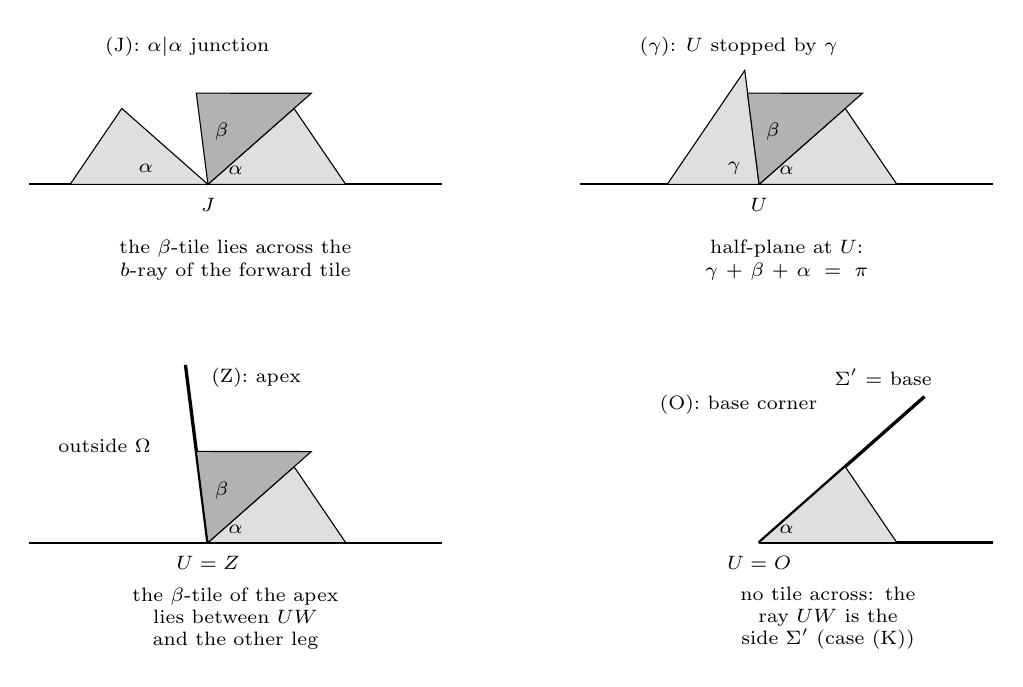
\begin{tikzpicture}[scale=1.75,font=\scriptsize]
  % tile data for (u,v)=(2,3), unit c: forward tile (0,0),(1,0),(0.625,0.551); beta tile (0,0),(0.75,0.661),(-0.084,0.662)
  \newcommand{\ftile}{\draw[fill=gray!25] (0,0)--(1,0)--(0.625,0.551)--cycle;}
  \newcommand{\btile}{\draw[fill=gray!60] (0,0)--(0.75,0.661)--(-0.084,0.662)--cycle;}
  % (J)
  \begin{scope}
    \draw[thick] (-1.3,0)--(1.7,0);
    \draw[fill=gray!25] (-1,0)--(0,0)--(-0.625,0.551)--cycle;
    \ftile \btile
    \node at (0,-0.15) {$J$}; \node at (-0.45,0.12) {$\alpha$}; \node at (0.2,0.1) {$\alpha$};
    \node at (0.1,0.38) {$\beta$};
    \node at (-0.15,1.0) {(J): $\alpha|\alpha$ junction};
    \node[text width=3.3cm,align=center] at (0.2,-0.55) {the $\beta$-tile lies across the $b$-ray of the forward tile};
  \end{scope}
  % ($\gamma$)
  \begin{scope}[xshift=4cm]
    \draw[thick] (-1.3,0)--(1.7,0);
    \draw[fill=gray!25] (-0.667,0)--(0,0)--(-0.104,0.827)--cycle;
    \ftile \btile
    \node at (0,-0.15) {$U$}; \node at (-0.18,0.12) {$\gamma$}; \node at (0.2,0.1) {$\alpha$};
    \node at (0.1,0.38) {$\beta$};
    \node at (-0.15,1.0) {($\gamma$): $U$ stopped by $\gamma$};
    \node[text width=3.3cm,align=center] at (0.2,-0.55) {half-plane at $U$: $\gamma+\beta+\alpha=\pi$};
  \end{scope}
  % (Z)
  \begin{scope}[yshift=-2.6cm]
    \draw[thick] (-1.3,0)--(1.7,0);
    \draw[very thick] (0,0)--(-0.163,1.29);
    \ftile \btile
    \node at (0,-0.15) {$U=Z$}; \node at (0.2,0.1) {$\alpha$};
    \node at (0.1,0.38) {$\beta$};
    \node at (-0.75,0.7) {outside $\Omega$};
    \node at (0.35,1.2) {(Z): apex};
    \node[text width=3.3cm,align=center] at (0.2,-0.55) {the $\beta$-tile of the apex lies between $UW$ and the other leg};
  \end{scope}
  % (O)
  \begin{scope}[xshift=4cm,yshift=-2.6cm]
    \draw[very thick] (0,0)--(1.7,0);
    \draw[very thick] (0,0)--(1.2,1.06);
    \ftile
    \node at (0,-0.15) {$U=O$}; \node at (0.2,0.1) {$\alpha$};
    \node at (0.9,1.2) {$\Sigma'$ = base};
    \node at (-0.15,1.0) {(O): base corner};
    \node[text width=3.3cm,align=center] at (0.5,-0.55) {no tile across: the ray $UW$ is the side $\Sigma'$ (case (K))};
  \end{scope}
\end{tikzpicture}
\caption{The four situations of Lemma~\ref{lem:leg}(b), at the point $U$ (or $J$) where the run starts, for $(u,v)=(2,3)$. Light: the first forward tile $\mathsf t_1$ of the run, with its edge $c$ on the leg and its edge $b$ on the ray $UW$ (angle $\alpha$ above the leg). In (J), ($\gamma$), (Z) a tile showing $\beta$ (dark) lies across the ray $UW$ and has an edge $a$ or $c$ on it: hypothesis (I) of Lemma~\ref{lem:rows}. In (O) the corner is filled by $\mathsf t_1$ alone and the ray is the other side of $\Omega_{\bar g}$ (bold), a wall for free: case (K).}\label{fig:cases}
\end{figure}

\begin{remark}[The run form and the general side; \sW]\label{rem:anyside}
Without the assumption that $\mathcal A$ has fewer than $u$ edges $c$, the same four cases show that \emph{every} $c$-run on a leg that is stopped at both ends has at least $u$ edges (at least $v$ in situation (O)), since each block used is a sub-block of the run. For the base, whose two ends are base corners, the same holds if $g\ge2$ (so that a leg is longer than $(v-1)b$). These run forms (c) and the statement for the base are written and not formalized; Theorem~F does not use them.
\end{remark}

\subsection{Theorem F}\label{sub:outline}
\begin{theorem}[Theorem F; \sF]\label{thm:Dprime}
{\small\noindent\emph{Lean:} \lean{ThmD.thmDStatement_geo}, \lean{ThmD.thmD_standalone}, \lean{ThmDGeoUnit.thmD_geo_unit}\par}
Let $u<v<2u$ be coprime, $d=v-u$, and $g\ge2$ an integer with $(g-1)d<u$. Then $\Omega_{g}$ has no tiling by the tile $(u^2,v^2-u^2,uv)$.
\end{theorem}
\emph{Outline.} (1) The $\alpha$-leg has an edge $b$, so its word has $m\le g-1$. (2) Hence its number of edges $c$ is $md<u$. (3) Lemma~\ref{lem:leg}(b): it has at least $u$ edges $c$. (4) Contradiction.
\begin{proof}
\textbf{Th1.} (This step and the next use no lower bound on $g$.) By Lemma~\ref{lem:apex} the $\alpha$-leg $A$ exists and has $\varepsilon_{\rm first}=\varepsilon_{\rm last}=0$; by Lemma~\ref{lem:counting} it has $n_b\ge1$. In the word $(md+jv,\,u(g-m),\,md-ju)$ of Lemma~\ref{lem:words} the number of edges $b$ is $u(g-m)$, so $m\le g-1$.
\textbf{Th2.} Then $md\le(g-1)d<u<v$. From $md+jv\ge0$ we get $j\ge-\lfloor md/v\rfloor=0$ and from $md-ju\ge0$ we get $j\le\lfloor md/u\rfloor=0$; so $j=0$ and $A$ has exactly $md<u$ edges $c$ (\lean{ThmDWords.leg_word_bound_D}).
\textbf{Th3.} By Lemma~\ref{lem:leg}(b) with $\bar g=g$, $A$ has at least $u$ edges $c$. This contradicts Th2.
\end{proof}
The Lean statement is the unit-scale form \lean{ThmDGeoUnit.thmD_geo_unit} (model and target with the sides above, $(g-1)d<u$), and \lean{ThmD.thmDStatement_geo} follows by rescaling; \lean{ThmD.thmD_all_g} states it for every $g\ge1$. Inside it the $\alpha$-leg is selected in the unit dissection (the apex dichotomy, \lean{ThmDGeoLegs.alpha_apex_leg_pos}), \lean{leg_c_count_S1} or \lean{leg_c_count_S2} gives $u\le n_c$ on it, and \lean{ThmDWords.leg_word_bound_D} the upper bound.

\begin{remark}[$g=1$ and sharpness; \sW, a reproduction]\label{rem:gone}
\emph{The case $g=1$.} The hypothesis $g\ge2$ of Theorem~F is not used in its proof. Th1 and Th2 hold for every integer $g\ge1$: for $g=1$ they read $m\le g-1=0$, so $m=0$, $j=0$, and the $\alpha$-leg has $n_c=0<u$ edges $c$. The leg lemma (b) holds for every real $\bar g\ge1$, because case (O) needs only $|\Sigma'|=\bar gvb>nb$, true for $\bar g\ge1$ and $n\le u-1<v$. So the written argument shows that $\Omega_{1}$ has no tiling by $(u^2,v^2-u^2,uv)$. This is Beeson's Theorem~11.7 \cite{BeesonIso}, the clause (G1) of Definition~\ref{def:Gtest}: the result is his, not new, and the route here (the run machinery, itself adapted from BR) is a different, longer one than his. In Lean the case $g=1$ is now also \lean{ThmD.thmD_g1}, the instance $g=1$ of \lean{ThmD.thmD_all_g} (standard axioms), next to the older arithmetic proof \lean{GPairArith.gPair_of_coprime}. The test $\mathrm G(N)$ does not change.

\emph{Sharpness.} Suppose $(g-1)d=u$ with $\gcd(u,v)=1$. Then $d\mid u$, and $\gcd(u,v)=\gcd(u,d)=d$, so $d=1$, $v=u+1$ and $g=u+1=v$. The smallest such targets are $\Omega_{3}$ at $(u,v)=(2,3)$ (tile $(4,5,6)$, $N=45$), $\Omega_{4}$ at $(3,4)$ (tile $(9,7,12)$, $N=112$) and $\Omega_{5}$ at $(4,5)$ ($N=225$). We know no tiling of any of them. For the first two there are finite float searches (\sS: all three orientations of the target, one search order, no certificate) that found no tiling; they are verdicts of a program, not theorems, and say nothing about $N$, since $45$ and $112$ are tile counts by other families. The tilings of $\Omega_{g}$ known to us (Section~\ref{sub:scope}) all have $v\mid g$ and $(g-1)d\gg u$. So the boundary $(g-1)d<u$ is the limit of the method, and Theorem~F is not known to be sharp.
\end{remark}

\begin{corollary}[Small scales: $g=2$ and $v=u+1$; \sF]\label{cor:small}
\textup{(a)} $\Omega_{2}$ has no tiling by any tile $(u^2,v^2-u^2,uv)$, $u<v<2u$ coprime. \textup{(b)} If $v=u+1$, then $\Omega_{g}$ has no tiling for $2\le g\le u$, that is for every $g<v$.
\textup{(c)} Theorem~F contains the case $gd<u$ (the case in which the word of the base is also bounded; $g=1$ is Beeson's \cite[Thm.~11.7]{BeesonIso}, \lean{GPairArith}), and adds exactly the scale $g=\lceil u/d\rceil$ for $d\ge2$ and $g=u$ for $d=1$.
\end{corollary}
\begin{proof}
(a) $(g-1)d=d<u$. (b) $(g-1)\cdot1<u$ iff $g\le u$. (c) $gd<u$ implies $(g-1)d<u$, and $(g-1)d<u\le gd$ exactly for $g=\lceil u/d\rceil$.
\end{proof}

\subsection{Scope and controls}\label{sub:scope}
\emph{Scope.} Theorem~F is stated for integer $g\ge2$ because $g=1$ is the known case (G1) (Beeson); the Lean theorem covers $g\ge1$. It says nothing when $(g-1)d\ge u$. Listing all coprime $u<v<2u$ and $g\ge2$ with $(g-1)(v-u)\ge u$ by $N=g^2(v^2-u^2)$ (exact enumeration), the first eight are
\[
\begin{array}{c|cccccccc}
N & 45 & 80 & 112 & 125 & 144 & 175 & 180 & 225\\
(u,v,g) & (2,3,3) & (2,3,4) & (3,4,4) & (2,3,5) & (3,5,3) & (3,4,5) & (2,3,6) & (4,5,5)
\end{array}
\]
and the next are $245$ at $(2,3,7)$, $252$ at $(3,4,6)$, $256$ at $(3,5,4)$, $297$ at $(4,7,3)$, $320$ at $(2,3,8)$. With $d\ge2$ the first are $144$ at $(3,5,3)$, $256$ at $(3,5,4)$, $297$ at $(4,7,3)$, $351$ at $(5,8,3)$, $384$ at $(5,7,4)$.
Theorem~F does not decide any of these targets (for $45$ and $112$ only float searches exist, Remark~\ref{rem:gone}). For the census status of these $N$ (recomputed exactly against the census dump and the list of known tile counts, \sS): all of them up to $252$, and $256$, $320$, $384$, $324$, $343$, $396$, $400$, $405$ are tile counts by other families. The first with census status \emph{undecided} are $297$ (failing leaves $\mathrm{Iso}$, $G$) and $351$ ($G$, $S_1$); the next is $816$ at $(7,10,4)$ (leaf $G$ only). The value $528=33\cdot4^2$ at $(4,7,4)$, which also has $(g-1)d\ge u$, is a tile count: it is $33m^2$ with $m=4$, a seed of the additive semigroup generated by $4$ and $9$ (Section~\ref{sec:herdt}, \lean{Iso357Semigroup.iso357_semigroup}); the program's dump lists it as undecided and the list of $1\,287$ values found later (Section~\ref{sec:census}) removes it.
Lemma~K is stated and used only for blocks that are stopped at the far end; nothing is claimed about a corner block that is not stopped.

\emph{What an enumeration of side words shows} (\sS; not used in any proof). An exact enumeration of the oriented side words of $\Omega_{g}$ under three rules, namely the fan rule at every junction and at the corners and the apex, Lemma~\ref{lem:leg} for runs stopped at both ends, and the bound $n\ge v$ of Lemma~K for corner runs, was run for all coprime pairs with $u\le8$ and $2\le g\le4$. It rejects every triple with $(g-1)d<u$, and every rejected triple is of this kind. It does not reject, for example, $(3,5)$ with $g=3$. So, within the rules listed, the method stops exactly at $(g-1)d<u$ on the pairs scanned. This is a statement about this scan, not a sharpness theorem.

\emph{Controls, and what they control.} The tilings of $\Omega_{g}$ known to us are: $g=15$ at $(2,3)$ (Herdt's, $1125$ tiles, published by Beeson \cite{BeesonIso}); $g=35$ at $(3,5)$ and $g=63$ at $(4,7)$ (Section~\ref{sec:herdt}); and Laczkovich's eight-piece construction, whose scale at $(2,3)$ is $g_0=v(u^4-u^2v^2+v^4)=3\cdot61=183$ (release paper, Section~``What is open''; our Lean theorem \lean{LaczFamily.lacz_family_uncond} is the uniform family with the multiples $2buv\,g_0$ of this scale, and we have no tile-level witness of $g=183$ itself). All have $v\mid g$ and $(g-1)d\ge u$, so Theorem~F is not contradicted, and they cannot test its hypothesis or its contradiction. What they test is the lemmas: the tilings with $19\,600$ and $130\,977$ tiles (Section~\ref{sec:herdt}) were checked to satisfy Lemma~\ref{lem:fan} at every point of every side, and the stopped runs they contain (lengths $80$ and $231$ on a leg, $45$ and $112$ from the apex; \sS) have more than $u$ edges, as Lemma~\ref{lem:leg} requires. Independently of the proof, the finite searches of the release paper exclude, for example, $N=132=33\cdot2^2$ ($(u,v)=(4,7)$, $g=2$) and $N=156=39\cdot2^2$ ($(5,8)$, $g=2$), both of which satisfy $(g-1)d<u$; this is consistent with Theorem~F and is not a check of its proof.

\section{The uniform Herdt family}\label{sec:herdt}

Herdt's tiling of the isosceles triangle with base angles $\alpha$ by $1125$ copies of the tile $(4,5,6)$, published by Beeson
\cite[Fig.~23]{BeesonIso}, is the only tiling of this target that was known before this work with a scale not produced by
Laczkovich's eight-piece construction. It is a \emph{macro-dissection}: the target is cut into seven triangles similar to the tile
(at the scales $12,8,10,10,8,12,15$) and four parallelograms with sides $b$ and $c$, each filled with a grid of cells, a cell being a parallelogram of two tiles.
This section shows that the same pattern of pieces exists for many tiles $(u^2,v^2-u^2,uv)$, derives the equations that decide when it closes, and states what is formal.
The instance $(2,3)$ is Herdt's and Beeson's; the family is ours.

\subsection{The pieces and the two equations}\label{sub:herdtpieces}
Let $u<v<2u$ be coprime, $a=u^2$, $b=v^2-u^2$, $c=uv$, $\rho=v/u$ and $\zeta=\cos\alpha+i\sin\alpha$, so that $\zeta+\zeta^{-1}=2\cos\alpha=\rho$. A point of the plane is written $(x,y)=x+y\zeta$ (oblique coordinates); the
squared length of $(x,y)$ is $x^2+\rho xy+y^2$, a vector of length $\lambda$ in the direction $\zeta^k$ is $\lambda \zeta^k$, and $\zeta^{-1}=(\rho,-1)$. For example the triangle with vertices $(0,0)$, $(c,0)$, $(0,b)$ has the sides $c$, $b$ and
$|(c,-b)|^2=c^2-\rho cb+b^2=u^4=a^2$, so it is the tile.
Let $D,\tau,n_1,k_1,n_2,k_2$ be positive integers and put
\[
g=v(D+\tau v),\qquad N=bg^2 .
\]
\emph{Scales:} $(s_1,\dots,s_7)=(uvD,\;u^2D,\;bD,\;\tau ub,\;\tau u^3,\;\tau u^2v,\;\tau vb)$.
\emph{Lengths:} $H=s_1b$, $\xi_1=n_1c+k_1b$, $\xi_2=\xi_1+s_1c$, $\xi_3=\xi_2+s_3b$, $Y=n_2c+uk_2b$, $\Lambda=gbv$.
\emph{Points:} $A=(0,0)$, $C=(\Lambda,0)$, $B=(0,gub)$ are the vertices of $\Omega_{g}$ (its base is $AC=gbv$, its legs $gub$);
$P_1=(n_1c,0)$, $P_2=(\xi_1,0)$, $P_3=(\xi_2,0)$, $P_4=(\xi_3,0)$, $P_1'=(n_1c,H)$, $P_2'=(\xi_1,H)$, $M_0=(0,H)$, $\mathrm{L}_0=(s_7b,H)$,
$E_3=(\xi_3-\rho n_2c,\,n_2c)$, $E_4=(\Lambda-\rho n_2c,\,n_2c)$, $Q_1=(\rho s_6c,\;gub-s_6c)$, $Q_2=(\Lambda-\rho Y,\,Y)$, $Q_3=(\Lambda-\rho Y-s_4c,\,Y)$.
The eleven pieces are the polygons of Table~\ref{tab:herdt}; the triangle $\Pi_i$ has the sides $s_ia,s_ib,s_ic$ (a direct computation with the length formula), and the parallelogram $\Xi_j$ has sides that are
integer multiples of $b$ and $c$ in the stated numbers.
\begin{table}[ht]
\centering\small
\begin{tabular}{llll}
\hline
piece & vertices & scale or grid & tiles\\
\hline
$\Pi_1$ & $P_2,\,P_3,\,P_2'$ & scale $s_1$ & $s_1^2$\\
$\Pi_2$ & $\mathrm{L}_0,\,P_2',\,P_3$ & scale $s_2$ & $s_2^2$\\
$\Pi_3$ & $P_4,\,\mathrm{L}_0,\,P_3$ & scale $s_3$ & $s_3^2$\\
$\Pi_4$ & $Q_2,\,Q_3,\,Q_1$ & scale $s_4$ & $s_4^2$\\
$\Pi_5$ & $Q_1,\,\mathrm{L}_0,\,Q_3$ & scale $s_5$ & $s_5^2$\\
$\Pi_6$ & $\mathrm{L}_0,\,Q_1,\,B$ & scale $s_6$ & $s_6^2$\\
$\Pi_7$ & $\mathrm{L}_0,\,B,\,M_0$ & scale $s_7$ & $s_7^2$\\
$\Xi_1$ & $A,\,P_1,\,P_1',\,M_0$ & $n_1$ cells of side $c$ by $s_1$ cells of side $b$ & $2n_1s_1$\\
$\Xi_2$ & $P_1,\,P_2,\,P_2',\,P_1'$ & $k_1$ cells of side $b$ by $s_3$ cells of side $c$ & $2k_1s_3$\\
$\Xi_3$ & $P_4,\,C,\,E_4,\,E_3$ & $s_6$ cells of side $b$ by $n_2$ cells of side $c$ & $2s_6n_2$\\
$\Xi_4$ & $E_3,\,E_4,\,Q_2,\,Q_3$ & $s_4$ cells of side $c$ by $uk_2$ cells of side $b$ & $2s_4uk_2$\\
\hline
\end{tabular}
\caption{The eleven pieces of the macro-dissection, in the oblique coordinates of Section~\ref{sub:herdtpieces}.}\label{tab:herdt}
\end{table}

\begin{figure}[ht]
\centering
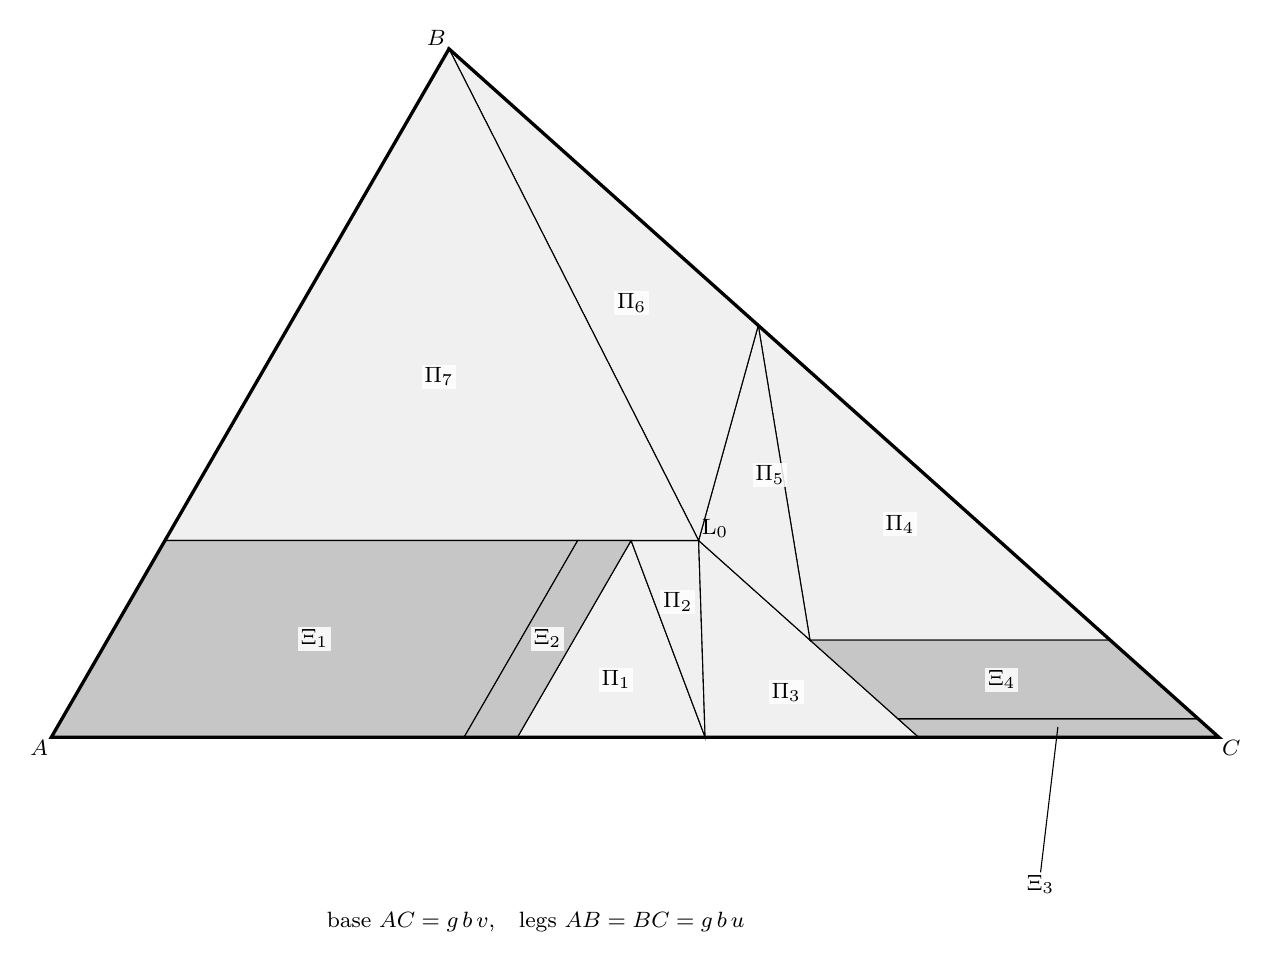
\begin{tikzpicture}[x={(0.0053cm,0cm)},y={(0.0030cm,0.0052cm)},
  tri/.style={draw,thin,fill=gray!12},par/.style={draw,thin,fill=gray!45},
  lab/.style={font=\footnotesize,inner sep=1pt,fill=white,fill opacity=0.85,text opacity=1}]
  \draw[tri] (1118,0) -- (1568,0) -- (1118,480) -- cycle;          % T1
  \draw[tri] (1280,480) -- (1118,480) -- (1568,0) -- cycle;        % T2
  \draw[tri] (2080,0) -- (1280,480) -- (1568,0) -- cycle;          % T3
  \draw[tri] (1125,1005) -- (1685,237) -- (2405,237) -- cycle;     % T4
  \draw[tri] (1125,1005) -- (1280,480) -- (1685,237) -- cycle;     % T5
  \draw[tri] (1280,480) -- (1125,1005) -- (0,1680) -- cycle;       % T6
  \draw[tri] (1280,480) -- (0,1680) -- (0,480) -- cycle;           % T7
  \draw[par] (0,0) -- (990,0) -- (990,480) -- (0,480) -- cycle;            % B1
  \draw[par] (990,0) -- (1118,0) -- (1118,480) -- (990,480) -- cycle;      % B2
  \draw[par] (2080,0) -- (2800,0) -- (2725,45) -- (2005,45) -- cycle;      % B3
  \draw[par] (2005,45) -- (2725,45) -- (2405,237) -- (1685,237) -- cycle;  % B4
  \draw[very thick] (0,0) -- (2800,0) -- (0,1680) -- cycle;
  \node[below left,lab,fill=none] at (0,0) {$A$};
  \node[below right,lab,fill=none] at (2800,0) {$C$};
  \node[above left,lab,fill=none] at (0,1680) {$B$};
  \node[lab] at (1275,140) {$\Pi_1$};
  \node[lab] at (1315,330) {$\Pi_2$};
  \node[lab] at (1700,110) {$\Pi_3$};
  \node[lab] at (1740,520) {$\Pi_4$};
  \node[lab] at (1360,640) {$\Pi_5$};
  \node[lab] at (790,1060) {$\Pi_6$};
  \node[lab] at (430,880) {$\Pi_7$};
  \node[lab] at (495,240) {$\Xi_1$};
  \node[lab] at (1054,240) {$\Xi_2$};
  \node[lab] at (2200,140) {$\Xi_4$};
  \draw[thin] (2400,25) -- (2560,-330) node[below,lab,fill=none] {$\Xi_3$};
  \node[above right,lab,fill=none] at (1280,480) {$\mathrm{L}_0$};
  \node[below,lab,fill=none] at (1400,-420) {base $AC=g\,b\,v$,\quad legs $AB=BC=g\,b\,u$};
\end{tikzpicture}
\caption{The macro-dissection of Section~\ref{sub:herdtpieces} at $(u,v)=(3,5)$, $(D,\tau,n_1,k_1,n_2,k_2)=(2,1,66,8,3,4)$, so $g=35$ and $N=bg^2=16\cdot35^2=19\,600$ ($b=16$, $c=15$).
The drawing is in the oblique coordinates $x+y\zeta$, so all vertices have integer coordinates; the plane picture is the image under a linear map and is not to scale in the Euclidean sense.
$\Pi_1,\dots,\Pi_7$ (light) are triangles similar to the tile, at the scales $30,18,32,48,27,45,80$, each cut into $s_i^2$ tiles; $\Xi_1,\dots,\Xi_4$ (dark) are grids of cells, each cell two tiles:
$\Xi_1$ is $66\times30$ cells, $\Xi_2$ is $8\times32$, $\Xi_3$ is $45\times3$, $\Xi_4$ is $48\times12$. The tile counts add to $\sum s_i^2+2\sum(\text{cells})=19\,600$.
The point $\mathrm{L}_0=(1280,480)$ is where $\Pi_2,\Pi_3,\Pi_5,\Pi_6,\Pi_7$ meet. With $(u,v)=(2,3)$ and parameters $(2,1,3,5,3,1)$ the same table gives $g=15$ and Herdt's $1125$ tiles.}
\label{fig:herdt}
\end{figure}

The vertices of Table~\ref{tab:herdt} are the incidence pattern of Herdt's picture, written with free parameters. The two equations that make the pieces fit are
\begin{align}
&b\,k_1+uv\,n_1+D\,u^4=\tau\,v\,b^2, \tag{E1}\\
&b\,k_2+v\,n_2+\tau\,u^4=D\,v\,b. \tag{E2}
\end{align}
(E1) says that the base closes: $\xi_3+s_6b=\Lambda$, that is the right end of $\Xi_3$ is $C$. Indeed $\xi_3+s_6b-\Lambda=n_1c+k_1b+D(u^2v^2+b^2-bv^2)+\tau(u^2vb-bv^3)=n_1c+k_1b+Du^4-\tau vb^2$, because $u^2v^2+b^2-bv^2=u^4$ and $u^2vb-bv^3=-vb^2$.
(E2) says that the side $BC$ closes: the point $Q_2+s_4b\,(-\rho,1)$ is $Q_1$, equivalently $Y+s_4b+s_6c=gub$, and $Y+s_4b+s_6c-gub=u\,(b k_2+vn_2+\tau u^4-Dvb)$ because $b^2+u^2v^2-bv^2=u^4$. The left side $AB$ closes
without a condition: $H+s_7c=uvbD+\tau uv^2b=gub$.

\begin{theorem}[Herdt's macro-dissection with parameters; \sF{}]\label{thm:herdtfamily}
{\small\noindent\emph{Lean:} \lean{HerdtFamily.herdt_family}.}
Let $u<v<2u$ be positive integers and let $D,\tau,n_1,k_1,n_2,k_2$ be positive integers satisfying \textup{(E1)} and \textup{(E2)}. Then $b\,(v(D+\tau v))^2$ is a tile count: $\Omega_{g}$ with $g=v(D+\tau v)$ has a tiling by the tile $(u^2,v^2-u^2,uv)$.
\end{theorem}
\begin{proof}
\emph{(1) Each piece is tiled.} A triangle with sides $s\,a,s\,b,s\,c$ is cut into $s^2$ tiles by the ladder dissection (\lean{Subdivision.ladderDissection}); a parallelogram with sides $b$ and $c$ and angle $\alpha$ is cut into two tiles by its diagonal $a$, and a grid of $m\times n$ such cells into $2mn$ tiles. The cells of $\Xi_1,\dots,\Xi_4$ have angle $\alpha$ or $\pi-\alpha$ between their sides, as needed.
\emph{(2) The pieces fit.} The pieces lie in $\Omega_{g}$ and have pairwise disjoint interiors. Each of the inequalities involved is linear in the oblique coordinates; they hold for all positive parameters satisfying \textup{(E1)}, \textup{(E2)} and the hypothesis $\nu>0$ derived in Proposition~\ref{prop:herdtdomain} below. These inequalities are verified in Lean, not by the reader's trust in a computation: the modules \lean{HerdtSep1} to \lean{HerdtSep4} prove them (the structure \lean{HP} lists them) for symbolic $(u,v)$ and parameters satisfying \textup{(E1)}, \textup{(E2)} and $\nu>0$, and for the instances below they were checked again in exact rational arithmetic. One representative, by hand. The triangles $\Pi_1=P_2P_3P_2'$ and $\Pi_2=KP_2'P_3$ share the edge $P_2'P_3$, so their interiors are disjoint iff $P_2=(\xi_1,0)$ and $\mathrm{L}_0=(s_7b,H)$ lie on opposite sides of the line $P_2'P_3$. In oblique coordinates the sign of the determinant $s_1c\,(y-H)+H\,(x-\xi_1)$ (a positive multiple of the Euclidean one, since $x+y\zeta\mapsto$ plane has positive determinant) decides the side of $(x,y)$. At $P_2$ it is $-s_1cH<0$; at $\mathrm{L}_0$ it is $H\,(s_7b-\xi_1)$, and $s_7b-\xi_1=\tau vb^2-(bk_1+uvn_1)=Du^4>0$ by \textup{(E1)}, because $s_7=\tau vb$, $\xi_1=n_1c+k_1b$ and $c=uv$. So $\Pi_1$ and $\Pi_2$ lie on opposite sides. The other separations and the containments are of the same kind, the sign of a linear form at a vertex; they are not written out here, and are the content of \lean{HerdtSep1}--\lean{HerdtSep4}.
\emph{(3) The areas add up.} In units of the area of the tile, the pieces have $\sum s_i^2+2(n_1s_1+k_1s_3+n_2s_6+uk_2s_4)$ tiles, and $\Omega_{g}$ has $bg^2$. Their difference is
\[
2D\,\bigl(bk_1+uvn_1+Du^4-\tau vb^2\bigr)+2\tau u^2\,\bigl(bk_2+vn_2+\tau u^4-Dvb\bigr),
\]
as a polynomial identity in $u,v,D,\tau,n_1,k_1,n_2,k_2$ with $b=v^2-u^2$ (\lean{HerdtFamily.herdt_family}, the step \texttt{linear\_combination}), so it vanishes by (E1) and (E2).
\emph{(4) Cover.} The union of the pieces is closed, lies in $\Omega_{g}$ and has the area of $\Omega_{g}$ by (3), and the pieces have disjoint interiors by (2); so the union is $\Omega_{g}$ (the rest of $\Omega_{g}$ would be a relatively open set of measure zero). Composing the tilings of (1) gives a tiling of $\Omega_{g}$ by $bg^2$ tiles (\lean{Compose.compose}).
\end{proof}

\subsection{When the system closes: the domain $(v^2-u^2)^3v^2>u^8$}
Write $\nu=b^3v^2-u^8$ (called $\mathrm{Vp}$ in the Lean files).
\begin{proposition}[\sW; written proof]\label{prop:herdtdomain}
{\small\noindent\emph{Lean:} \lean{herdt_family}, \lean{herdt_uniform}\par}
(The proposition is not a Lean statement; its algebra is a step of the two Lean proofs named above.) Let $u<v<2u$ be positive integers. \textup{(a)} If positive reals $D,\tau,n_1,k_1,n_2,k_2$ satisfy \textup{(E1)} and \textup{(E2)}, then $\tau \nu =vb\,(bk_1+uvn_1)+u^4(bk_2+vn_2)>0$, hence $\nu >0$.
\textup{(b)} If $\nu >0$, then
\[
\tau=2bv\,(u^4+buv),\quad D=2\nu +2u^4(u^4+buv),\quad k_1=uv\nu ,\quad n_1=b\nu ,\quad k_2=v\nu ,\quad n_2=b\nu 
\]
are positive integers satisfying \textup{(E1)} and \textup{(E2)}, and every positive integer multiple of this solution is again one. The corresponding scale is $g=v(D+\tau v)=2v\bigl(\nu +(u^4+buv)(u^4+bv^2)\bigr)=:g_0$.
So \textup{(E1)}, \textup{(E2)} have a solution in positive reals if and only if $(v^2-u^2)^3v^2>u^8$, and then they have solutions in positive integers.
\end{proposition}
\begin{proof}
(a) Multiply (E1) by $vb$ and (E2) by $u^4$ and add: $vb(bk_1+uvn_1)+Du^4vb+u^4(bk_2+vn_2)+\tau u^8=\tau v^2b^3+Du^4vb$, that is $vb(bk_1+uvn_1)+u^4(bk_2+vn_2)=\tau(v^2b^3-u^8)=\tau \nu $. The left side is positive.
(b) $bk_1+uvn_1=2buv\nu $, so (E1) reads $2buv\nu +Du^4=\tau vb^2$; with the given $D$ and $\tau$ the left side is $2\nu (u^4+buv)+2u^8(u^4+buv)=2(u^4+buv)(\nu +u^8)=2(u^4+buv)\,b^3v^2$, which equals $\tau vb^2=2b^3v^2(u^4+buv)$. Similarly $bk_2+vn_2=2bv\nu $ and (E2) reads $2bv\nu +\tau u^4=Dvb$, true because $Dvb=2bv\nu +2bvu^4(u^4+buv)$. The formula for $g_0$ is the substitution. Both equations are linear and homogeneous in the six unknowns, so integer multiples of a solution are solutions.
\end{proof}
\begin{theorem}[Herdt's macro-dissection, uniform in the tile; \sF{}]\label{thm:herdt}
{\small\noindent\emph{Lean:} \lean{HerdtFamily.herdt_uniform}.}
Let $u<v<2u$ be positive integers with $(v^2-u^2)^3v^2>u^8$, $b=v^2-u^2$, $\nu =b^3v^2-u^8$ and $g_0=2v\bigl(\nu +(u^4+buv)(u^4+bv^2)\bigr)$. Then $\Omega_{sg_0}$ has a tiling by the tile $(u^2,v^2-u^2,uv)$ for every
$s\ge1$; that is, $b\,(sg_0)^2$ is a tile count.
\end{theorem}
\begin{proof}
Theorem~\ref{thm:herdtfamily} applied to $s$ times the solution of Proposition~\ref{prop:herdtdomain}(b) (\lean{herdt_uniform} does exactly this, with the six values as given there).
\end{proof}
At $(u,v)=(2,3)$: $b=5$, $\nu =1125-256=869$, $g_0=6(869+46\cdot61)=22\,050$, while Herdt's tiling has $g=15$; the uniform $g_0$ is a convenient positive solution, not the least one. For the actual least scale of the pieces of Table~\ref{tab:herdt} one searches for the least $g=v(D+\tau v)$ for which (E1), (E2) have positive integer solutions $(n_1,k_1,n_2,k_2)$; such a search (\sS, exact integer arithmetic, $g\le2000$, recomputed for this paper) gave the least $g=15,35,63,84,88,108,160$ for $(u,v)=(2,3),(3,5),(4,7),(5,7),(5,8),(5,9),(7,10)$, against the scales $v(u^4-u^2v^2+v^4)=183,\ 2405,\ 13\,111,\ 12\,607,\ 24\,968,\ 46\,449,\ 75\,010$ of Laczkovich's family at the same pairs (ratios $12$, $69$, $208$, $150$, $284$, $430$, $469$).

\paragraph{Pairs outside the domain.} For $v=u+1$, $u\ge3$: $b=2u+1\le\frac73u$ and $v\le\frac43u$, so $b^3v^2\le\frac{343}{27}\cdot\frac{16}{9}u^5<23u^5\le u^8$ for $u\ge3$; hence the pairs $(u,u+1)$ with $u\ge3$ are outside the domain, and $(2,3)$ is inside ($1125>256$). Other pairs outside: $(7,9)$ ($32^3\cdot81=2\,654\,208<7^8=5\,764\,801$), $(9,11)$, $(10,13)$. For these pairs this macro-dissection does not close; no tiling of $\Omega_{g}$ with $v=u+1$, $u\ge3$ is known to us.

\paragraph{What is computed and not proved here (\sS).} The incidence pattern of Herdt's instance, counted by a program from its vertex list at $(2,3)$, has $14$ groups of coinciding vertices, $10$ vertices lying inside an edge of another piece, and $26$ vertices on the sides of the target. Taking the seven scales, the eight side lengths of the grids and the positions of the pieces as unknowns, every incidence is a linear equation over $\Q(v/u)$ in oblique coordinates; an exact solve for the coprime pairs with $u\le11$ inside the domain gave a four-dimensional solution space, which is the family above (six integer unknowns and two equations). The statements \textup{(a)}, \textup{(b)} of Proposition~\ref{prop:herdtdomain} are for the system (E1), (E2) and do not rely on this solve; what the solve adds is that no other solution of the incidences exists, which no theorem here needs. The positivity test of the full system agreed with $\nu >0$ on all $127$ coprime pairs with $u\le20$.
The same inequality $(v^2-u^2)^3v^2>u^8$ is the domain of Laczkovich's eight-piece family on those $127$ pairs (\sS; formalized in the library as \lean{LaczFamily.lacz_family_uncond}); we have no explanation for the coincidence, and the scales of that family are much larger (ratios in the preceding paragraph).

\subsection{Instances, controls and what they control}
The instances $(u,v)=(3,5)$ at $g=35$, with $19\,600$ tiles ($(D,\tau,n_1,k_1,n_2,k_2)=(2,1,66,8,3,4)$), and $(4,7)$ at $g=63$, with $130\,977$ tiles ($(2,1,241,11,20,2)$), are the first tilings of
this target with $u\ge3$ at a scale below $10^6$ tiles. Both are Lean theorems (\lean{HerdtFamily.tileCount_19600}, \lean{tileCount_130977}) and were verified at tile level in exact arithmetic (every tile congruent to the model, the areas, containment, pairwise disjointness over $224\,659$ and $1\,681\,191$ candidate pairs, no overlap). The control $(2,3)$ with parameters $(2,1,3,5,3,1)$ gives Herdt's $1125$ (\lean{tileCount_1125}).
These controls test the \emph{construction} (that the stated pieces tile $\Omega_{g}$); they do not test the hypothesis $(g-1)d<u$ of Theorem~F, which none of the instances satisfies (their $g$ are multiples of $v$ far above $u/d$).
In every member no side of $\Omega_{g}$ carries an edge $a$ (the pieces put only edges $b$ and $c$ on the sides); this is the observation cited as evidence for the conjecture of the release paper that no tiling of $\Omega_{g}$ has an edge $a$ on a side.

\paragraph{Effect on the census.} The family adds no new tile count below $10^6$. The three instances with $N\le10^6$ that we computed are already tile counts of the census: $1125=33^2+6^2$ is a sum of two squares, $19\,600=140^2$ is a square, and
$130\,977=33\cdot63^2$ is $33m^2$ with $m=63=7\cdot9$ in the additive semigroup generated by $4$ and $9$. The last is a fact of the release paper \cite{ReleasePaper}: gluing equilateral triangles tiled by the tile $(3,5,7)$ (seeds $m=4$ and $m=9$, of sides $15m$) gives such a tiling for every $m$ in the semigroup, and two further tiles give the isosceles triangle $(21m,21m,33m)$ with $33m^2$ tiles (release paper, \S6; \lean{Iso357Semigroup.iso357_semigroup}).
For every pair the uniform scale $g_0$ gives $N>10^6$. The instance and its publication are Herdt's and Beeson's; the family is ours.


%=====================================================================
% SECTION: THE CENSUS
%=====================================================================

\section{The census to one million}\label{sec:census}

\subsection{What a census value means}
For a non-squarefree $N$ the classification of Section~\ref{sec:reduction} reduces the question ``is $N$ a tile count'' to finitely many
\emph{branches}. A branch is a family of pairs (target, tile) with sides given by integer parameters, and for each branch the number of tiles
is a known function of the parameters, so the instances of a branch with exactly $N$ tiles can be listed. For each branch the library has a \emph{leaf}: a theorem of the form
\[
\begin{array}{c}\text{(a decidable condition on the instances of the branch with $N$ tiles)}\\ \Longrightarrow\ \text{no tiling of $N$ tiles in that branch}.\end{array}
\]
There are fifteen branches and fifteen leaves; Table~\ref{tab:leaves} lists them with one line each. The leaf for a branch \emph{excludes} the branch for $N$ when its condition holds.
Four of the leaves are called \emph{obstruction classes}, because they are the ones that fail for most of the undecided values: $S_1$, $S_4$, $G$ and $S_5$ (the first three are explained next; $G$ and $S_5$ are the tests $\mathrm{G}(N)$ and $\mathrm{W}(N)$ of Section~\ref{sec:reduction}). The other eleven are the \emph{minor leaves}.

\paragraph{The base-$\psi$ targets (leaves $S_1$ and $S_4$).} The targets $\mathcal B_\mu(e,f)$ and $\mathcal W_\mu(e,f)$ and the facts (B1)--(B3) are stated in Section~\ref{sub:typeT} (these are the ``base-$\beta$'' and ``cevian'' targets of the release paper, where the angle $\psi$ is called $\beta$). The leaf $S_1$ concerns $\mathcal B_\mu$ and the leaf $S_4$ concerns $\mathcal W_\mu$ at integer scales $\mu\ge2$: by (B1) a tiling exists for $\mu\ge f$, by (B2) and (B3) there is none in the ranges stated there, and the scales $2\le\mu<f$ outside them are open (apart from $\mathcal W_2(3,5)$); they are what the leaves $S_1$ and $S_4$ cannot decide.
The condition of $S_1$ in the Lean chain is the strongest that needs no run theorem: \emph{no} instance $N=\mu^2(3f^2-e^2)$ with $\mu\ge2$ exists (\lean{NSQChk.S1Chk}). The program also accepts $N$ when every such instance has $2\mu e<f$ (by (B2)); this is the sharpening of Section~\ref{sub:status} below, and it is not part of the Lean chain.

\paragraph{The final chain.}
The \emph{final chain} is the conjunction $\mathrm{CN'zETWD}(N)$ of the fifteen leaves, in which five leaves are in their sharpened forms (the letters of the name): \textup{z}, the leaf of the $2\pi/3$ scalene tiles uses a square-discriminant test;
\textup{E}, the equilateral leaf uses the irrationality of the $\pi/3$ pairs with a non-square discriminant (\lean{E60Irr.e60Pair_of_not_isSquare}); \textup{T}, the leaf $S_4$ uses (B2) and (B3) (\lean{NSQRWT.RWChkT}: every instance $(\mu,e,f)$ of $N=\mu^2(2f^2-e^2)$ has $\mu e<f$ or $\mu(f-e)\le e$);
\textup{W}, the leaf $S_5$ is the word test $\mathrm{W}(N)$; \textup{D}, the leaf $G$ is the test $\mathrm{G}(N)$, which contains Theorem~F. The theorem is \lean{NSQM.not_tile_of_conditionsNSQzETWD}: for every $N$, if $\mathrm{CN'zETWD}(N)$ holds then $N$ is not a tile count.
The condition is decidable and the kernel can evaluate it for a given $N$, as the witnesses $\mathrm{CN'zETWD}(168)$ and $\neg\mathrm{CN'zETWD}(72)$ show, but evaluating it for every $N\le10^6$ in Lean is
not feasible. A program (the Rust program \texttt{allncond2} of the release repository) evaluates the same condition and reports the list of $N$ for which it holds. The program is not
trusted for the mathematics: what it computes is the value of a predicate whose soundness is a theorem. It is checked against a literal triple loop over the definitions for all $N\le3000$, against the Lean witnesses (including those of Section~\ref{sub:fourvalues}), and against
the decided values $N\le200$ (the $105$ tile counts and the exclusions); each check has $0$ mismatches.

\begin{table}[ht]
\centering\small
\begin{tabular}{lp{5.2cm}p{5.6cm}}
\hline
leaf & pairs (target, tile) it closes & what it checks, in words\\
\hline
$B$ & commensurable or right-angled tiles & a condition on the squarefree part of $N$\\
$A$ & commensurable tiles & $N$ has a prime factor $p\ge7$ to an odd power\\
$\mathrm{NSq}$ & tile similar to the target & $N$ is not a sum of two squares\\
$\mathrm{HAr}$ & counts of the forms $2r^2,3r^2,6r^2,10r^2$ & arithmetic of those forms\\
$R$ & counts with $N/2$ a sum of two squares & $N$ odd, or $N/2$ not a sum of two squares\\
$E$ & equilateral targets, $\pi/3$ and $2\pi/3$ pairs & the commensurability relations and the irrationality leaf above\\
$F_1$ & $2\pi/3$ scalene tiles, family $F_1$ & $N\equiv2\pmod4$, or no admissible divisor pair\\
$S_2$ & targets with angles $(2\varphi,\varphi,2\psi)$ of the tile of type (T) & no admissible coprime $(p,q)$\\
$S_3$ & the isosceles targets $(\varphi,\varphi,\varphi+2\psi)$ of the tile of type (T) (base angles $\varphi$, apex $\varphi+2\psi$; the fifth target shape of Proposition~\ref{prop:types}) & no admissible integer parameters\\
$\mathrm{Iso}$ & $2\pi/3$ isosceles tiles & no admissible parameters\\
$R_8$ & $2\pi/3$ scalene tiles, families $F_2,F_3,F_4$ & no admissible parameters\\
$G$ & tile $(u^2,v^2-u^2,uv)$, $\gamma=2\alpha$, target $\Omega_{g}$, $N=g^2(v^2-u^2)$ & $\mathrm{G}(N)$ (Definition~\ref{def:Gtest}): every pair satisfies (G1), (G2) or (G3)\\
$S_1$ & base-$\psi$ targets $\mathcal B_\mu(e,f)$ at a scale $\mu\ge2$ & no instance with $N$ tiles (the program also: every instance has $2\mu e<f$)\\
$S_4$ & cevian targets $\mathcal W_\mu(e,f)$ at a scale $\mu\ge2$ & every instance has $\mu e<f$ or $\mu(f-e)\le e$\\
$S_5$ & $\theta$ targets $\theta_t(e,f)$, $t\ge2$ & $\mathrm{W}(N)$: no word $teb=xa+yb+zc$ with $z\ge f$ (\lean{NSQMS5W.S5wChk})\\
\hline
\end{tabular}
\caption{The fifteen leaves of the final chain. ``No admissible parameters'' means that the integer equations of that family have no solution with $N$ tiles; the families $F_1,\dots,F_4$, $S_2$, $S_3$ and the equations are in the release paper (they are not used elsewhere in this paper). The four leaves $S_1,S_4,G,S_5$ are the \emph{obstruction classes}; the other eleven are the \emph{minor leaves}.}\label{tab:leaves}
\end{table}

\subsection{The four obstruction classes, in words}
\begin{itemize}
\item \emph{The base-$\psi$ targets $\mathcal B_\mu(e,f)$ and $\mathcal W_\mu(e,f)$} (leaves $S_1$ and $S_4$): facts (B1)--(B3) above. The unresolved scales are $2\le \mu<f$.
\item \emph{The $\theta$ targets} (leaf $S_5$). The base carries $f$ consecutive
tiles with the edge $c$ on it, so $teb=xa+yb+zc$ with $z\ge f$ (Proposition~\ref{prop:theta}). The leaf
decides, for each instance, whether such $(x,y,z)$ exist, by a bounded search over $z$ and a congruence in $y$
(\lean{NSQMS5W.S5wChk}); the earlier closed-form corollaries $te\ge2f$ and $t\ge f+2$ (for $e=f-1$) are special cases, and the four tilings of
$\theta$ targets with $48$, $108$, $300$, $320$ tiles fail the condition, as they must.
\item \emph{The target with base angles $\alpha$ of the tile $(u^2,v^2-u^2,uv)$} (leaf $G$). The test $\mathrm{G}(N)$ of Definition~\ref{def:Gtest}, whose case (G3) is Theorem~F, as the decidable test $(g-1)(v-u)<u$ on each pair
(\lean{ThmD.thmD_standalone}, pair form).
\end{itemize}

\subsection{The formal status of the exclusions}\label{sub:status}
Version 2.0 has one Lean theorem for all the exclusions. Its hypothesis $\mathrm{CN'zETWDS}$ (\lean{ThmDChainWS.CN'zETWDS}) is the conjunction of the decidable leaf checks; it contains $G$ as $\mathrm G(N)$ (\lean{ThmD.GammaChkD}), $S_1$ in the form ``\lean{S1Chk} or \lean{S1tChk}'', where \lean{S1tChk} is the sharpened leaf ``every instance has $2\mu e<f$'' (Corollary on $2Me<f$ of the library), $S_4$ with (B2) and (B3) (\lean{RWChkT}) and $S_5$ as $\mathrm{W}(N)$ (\lean{S5wChk}). The theorem is
\lean{NSQM.not_tile_of_conditionsNSQzETWDS}: if $\mathrm{CN'zETWDS}(N)$ holds, then $N$ is not a tile count.
All $199\,140$ excluded values satisfy it. (In version 1.13.1 the exclusions were split as $196\,273+2\,867$, the second set needing the sharpening of $S_1$ that the program applied and the theorem then did not contain; the new theorem contains it, and the split is gone.) Of the $199\,140$, $62\,150$ already satisfy the hypothesis of the earlier theorem \lean{NSQMMainZET.not_tile_of_conditionsNSQzET}; for the others the new $G$ test, the word test or the sharpened $S_1$ leaf is used.
The condition is evaluated for each $N$ by a program (\texttt{nsq.rs}), not by the kernel; the kernel evaluates it, by \texttt{decide +kernel}, only for the values for which a witness is in the library (Section~\ref{sub:fourvalues}, and $428$, $204$, $228$). Evaluating the program's verdict for every $N$ inside Lean is not done. \sS

\subsection{The numbers}
Of the $392\,074$ non-squarefree $N\le10^6$:
\begin{itemize}
\item $199\,140$ are excluded, all by the hypothesis of the single theorem \lean{not_tile_of_conditionsNSQzETWDS} (Section~\ref{sub:status}). Of the $199\,140$, $71\,039$ were already excluded by the program of the previous release ($62\,150$ by the earlier single theorem and $8\,889$ with sharpenings) and $128\,101=199\,140-71\,039$ are new with Theorem~F and the word leaf.
The condition is evaluated by the program, not by the kernel.
\item $102\,613$ are tile counts, by the existence families of the library: those of the theorem on $N\le200$ (squares, sums of two squares, $3k^2$, $6k^2$, $7m^2$, $11m^2$ and the sporadic values), the formal families $S_2$, $F_3$, $F_4$ and the base-$\psi$ tilings of scale $\mu\ge f$, all scaled by
squares, the further tilings of the release paper, and Section~\ref{sec:herdt}.
\item $90\,321$ are undecided.
\end{itemize}
The program reports for each undecided value the set of leaves that fail. The $90\,321$ values (the program's $91\,750$ minus the $1\,429$ later found to be tile counts: $1\,287$ by the known families, $134$ by the family theorems of Paliy's nested corners of Section~\ref{sec:new21}, and $8$ by exact verification of template tilings, Section~\ref{sec:new21}) are partitioned
exactly, by the set of failing leaves, as follows: $S_1$ stands for the base-$\psi$ leaf at a scale $2\le \mu<f$, $S_4$ for the leaf of the targets $\mathcal W_\mu$ at such a scale, $G$ for the target with base angles $\alpha$ at a scale
$g\ge\lceil u/d\rceil+1$ (so Theorem~F does not apply), $S_5$ for a $\theta$ target whose word exists.

\begin{center}
\begin{tabular}{p{10.5cm}r}
\hline
failing leaves & values\\
\hline
$S_1$ only & 28\,615\\
$S_4$ only & 18\,619\\
$G$ only & 10\,964\\
$S_5$ only & 2\,468\\
\emph{one obstruction class only, subtotal} & \emph{60\,666}\\
$G,S_5$ & 16\,971\\
$S_1,S_4$ & 3\,426\\
$G,S_4,S_5$ & 1\,108\\
$G,S_1,S_5$ & 895\\
$G,S_4$ & 877\\
$G,S_1$ & 857\\
other subsets of $\{S_1,S_4,G,S_5\}$ with at least two elements ($S_4S_5$ 295, $S_1S_5$ 197, $GS_1S_4S_5$ 90, $GS_1S_4$ 70, $S_1S_4S_5$ 21) & 673\\
\emph{obstruction classes only (no minor leaf), subtotal} & \emph{85\,473}\\
minor leaves only ($S_3$ 765, $\mathrm{Iso}$ 493, $E F_1$ 240, $E$ 226, $R_8$ 128, $A$ 85, other 43) & 1\,980\\
minor leaves together with at least one obstruction class & 2\,868\\
\hline
total undecided & 90\,321\\
\hline
\end{tabular}
\end{center}
Thus the four counts $28\,615$, $18\,619$, $10\,964$, $2\,468$ (values for which \emph{one} obstruction class is the only failing leaf) account for $60\,666$ values; the remaining $29\,655$ either fail several obstruction classes and no minor leaf ($24\,807$) or involve a minor leaf
($4\,848$: $1\,980$ with minor leaves only and $2\,868$ with an obstruction class as well). The partition was recomputed from the program's output for the final chain (exact integers; \sS), and the sums above were checked.

Among the $128\,101$ values that are new with Theorem~F and the word leaf, the smallest are $171$, $204$, $228$, $276$, $279$, $304$, $315$, $348$, $372$, $380$, $387$, $459$. (The value $171$ is below $200$ and is also decided by the theorem on $N\le200$; the census counts it as excluded by the chain.) At the program's previous tier, in which the $\theta$ branch is closed by the two closed-form bounds, the first eleven fail only the leaf $G$ and $459$ is the smallest that fails $G$ and the closed-form $\theta$ leaf; the word leaf is needed there because the instance $(3,7,10)$ of $459$ has $te=21\ge2f=20$ and $e\ne f-1$, and $te\,b=1071$ admits no word with $z\ge10$. In terms of the single Lean theorem the picture is different: each of them fails both the earlier $G$ test and the earlier parity test for $S_5$, so the theorem uses Theorem~F (or (G2)) and the word test together. For $204$, $268$, $276$, $279$ this is a kernel statement (Section~\ref{sub:fourvalues}). The value $268$ is not new: it was already excluded by the program of the previous release (its pair is of the form (G2)), and is listed in Section~\ref{sub:fourvalues} only as a control; \lean{NSQM.cnzETWD_268}, like \lean{NSQM.cnzETWD_204}, \lean{NSQM.no_dissection_276} and \lean{NSQM.cnzETWD_279}, is a check of the final chain on that value. The
condition fails at the tile counts $72$, $143$, $320$ (\lean{NSQM.not_cnzETWD_72}, \lean{NSQM.not_cnzETWD_143},
\lean{NSQM.not_cnzETWD_320}), as it must.

\subsection{What the census is not}
It is not a description of the set of tile counts above $200$. It is the list of what the present theorems decide, with the
undecided values sorted by the leaf that resists. The obstruction classes $S_1$, $S_4$, $G$, $S_5$ contain both tile counts and excluded values at
the scales already decided, so no class can be removed by a statement about a branch as a whole; each needs a theorem about the
scales below the threshold (for the base-$\psi$ targets, the question of which scales $2\le \mu<f$ have a tiling, posed as an open question in the release paper, is the first of them).


%=====================================================================
\section{What is new in version 2.2}\label{sec:new22}
Relative to version 2.1 (release 1.15). The prime case is unchanged: nothing here bears on Theorem~1.1 or on the base-$\beta$ question.
\begin{itemize}
\item \textbf{Eight template tile counts are now Lean theorems} (\sF): $11\,625$, $66\,960$, $119\,040$, $121\,765$, $167\,865$, $186\,000$, $364\,560$, $603\,750$, each as \lean{TileCount} $N$ (declarations \texttt{tileCount\_$N$} in \texttt{Draft/T$N$}, with the generic module \texttt{Draft/LadderFam}, aggregate \texttt{Draft/AllTemplates}, in \texttt{AllR8}); standard axioms, no \texttt{sorry}, no \texttt{native\_decide}, no tile list. Tiles: $(4,15,16)$ for six of them, $(6,35,36)$ for $121\,765$, $(10,21,25)$ for $603\,750$. The proof assembles the target from a few convex pieces (similar triangles and trapezoids found by our template engine), each tiled by cells of the ladder subdivision (\lean{LadderFam.ladderFam}), and obtains the covering from an area identity. Credits: our engine for the templates; the skew-frame layer is a reconstruction of Beeson--Ro\c{s}u III, Theorem~10; the macro dissections are of Laczkovich type; the multiplicative scaling follows Paliy's families. A statement-match audit (the Lean statement is the census statement $\mathrm{TileCount}\,N$; the model tile is the stated one) was made within this work, no outside reader. In the census these eight values are unchanged ($102\,613$ tile counts); only their label moves from \sS{} to \sF. The five values above $10^6$ remain \sS.
\item \textbf{Evidence on the one-leg $W_3^+$ words at $g=3$} (type \sS, \emph{evidence only}; a conditional exact search with the filters named in the project notes, no Lean certificate). For the pairs $(u,v)=(4,7)$ and $(5,8)$ the word lists are complete ($191\,940$ and $84\,462$ words); every word was decided ``no tiling'' within $2$~s except $323$ and $630$ words; a uniform sample of those, run for $120$~s, decided about half of them, which extrapolates to roughly $160$ and $315$ words still unresolved (an extrapolation, not a count). No tiling was found for any word. For $(7,12)$ there are $8.4\cdot10^9$ words and only a uniform sample of $19\,999$ was run: $19\,994$ ``no tiling'', $5$ unresolved, none found. The conjecture is therefore neither refuted nor proved by this census, and the unresolved words are open.
\item \textbf{Housekeeping:} a private-path comment was removed from \texttt{rust/bonfioli\_template/src/search.rs}.
\end{itemize}

%=====================================================================
\section{What is new in version 2.1}\label{sec:new21}
Relative to version 2.0 (release 1.14), this version records the following, each with its standing. The prime case is unchanged: nothing here bears on Theorem~1.1 or on the base-$\beta$ question.
\begin{itemize}
\item \textbf{Three family theorems of D.~Paliy's nested-corner layouts, formalized} (\sF; the constructions are Paliy's, the Lean proofs are ours): for naturals $0<b<a$ and $c^2=a^2+ab+b^2$ (the tile with sides $a,b,c$ and angle $2\pi/3$ opposite $c$), \lean{PRevAll.prev_family} gives a tiling with $(2a+b)(a+b)$ tiles if $bc-a^2\in\langle a,b,c\rangle$; \lean{PF2All.pf2_family} gives $(a+2b)(2a+b)$ tiles under the same hypothesis; \lean{PF3All.pf3_family} gives $3(a+b)(a+2b)$ tiles if $a<2b$, with no semigroup hypothesis. Each is a statement $\mathrm{TileCount}(\cdot)$ (a tiling of some triangle by that many congruent copies of some triangle), proved for all admissible $(a,b,c)$ and all semigroup witnesses, with the standard axioms; they are in the aggregate \texttt{AllR8}, which contains no search certificate. A statement-match audit (hypotheses, conclusion, non-vacuity by $22$ instances) was made within this work only.
\item \textbf{All $22$ squarefree $R_8$ values are now Lean theorems}: $345, 506, 12\,922, 18\,602, 25\,179, 35\,763, 57\,479, 65\,626, 135\,746, 146\,982, 156\,647, 196\,251, 201\,122, 247\,494, 388\,847, 397\,371, 428\,978, 538\,346, 624\,338, 686\,945, 746\,327, 914\,529$ are instances of the three theorems (declarations \texttt{tileCount\_$N$} in \texttt{PRevAll}, \texttt{PF2All}, \texttt{PF3All}; $8$, $8$ and $6$ values). Squarefree $N\le10^6$ still open: $771$ at both levels.
\item \textbf{$134$ further non-squarefree values are tile counts.} Among the $91\,750$ undecided non-squarefree $N\le10^6$ of the program, $135$ equal $(2a+b)(a+b)k^2$, $(a+2b)(2a+b)k^2$ or $3(a+b)(a+2b)k^2$ for admissible $(a,b,c)$ ($79$, $22$ and $34$ values); one of them was already known. They follow from a family theorem and the scaling lemma \lean{TileCountFamilies.tileCount_scale}, with $(a,b,c)$ found by search; no separate Lean theorem is stated for each of them, so the count is of type \sS. For the census it makes no difference whether the finite list is proved value by value. The older families $F_3$, $F_4$ ($a<b$) already covered $382$ values of the program's undecided list; these were already among the $1\,287$ removed in version 2.0 and are not new.
\item \textbf{Eight values from a template engine, by exact verification} (type \sS in version 2.1; the eight values $\le10^6$ became Lean theorems in version 2.2, Section~\ref{sec:new22}; the five above $10^6$ remain \sS): $11\,625$, $66\,960$, $119\,040$, $121\,765$, $167\,865$, $186\,000$, $364\,560$, $603\,750$ (in the census), and $1\,071\,360$, $1\,183\,350$, $1\,545\,600$, $1\,904\,640$, $2\,779\,136$ (above $10^6$). Each is a tiling found by a search over macro-pieces (similar triangles, bricks, trapezoids) with integer scales, expanded to the individual tiles and checked by an independent exact verifier (congruence of every tile, containment, pairwise disjoint interiors, equal areas); the tilings are in \texttt{data/witnesses/}. Each decides only its own value $N=N_0g^2$; the squarefree cores $465$, $966$, $2\,485$ and $2\,714$ remain open. No hit for these numbers was found in the public claim ledger or papers of Paliy; his archive of $220$ files was not read.
\item \textbf{Census} of the $392\,074$ non-squarefree $N\le10^6$: $199\,140$ excluded (unchanged), $102\,613$ tile counts ($+142$: $134$ by the family theorems, $8$ by templates), $90\,321$ undecided. The counts are recomputed from the label files by a script that first reproduces the figures of version 2.0 ($102\,471$ and $90\,463$).
\end{itemize}

\section{What is new in version 2.0}\label{sec:new}
Relative to the first full draft of this paper and to release 1.13.1 of the library, this version records the following, each with its standing.
\begin{itemize}
\item \textbf{Theorem~F for every $g\ge1$ in Lean} (\sF): \lean{ThmD.thmD_all_g} and, for $g=1$, \lean{ThmD.thmD_g1}. The case $g=1$ reproduces Beeson's Theorem~11.7 \cite{BeesonIso}; it is credited to him.
\item \textbf{One theorem for all $199\,140$ non-squarefree exclusions up to $10^6$} (\sF{} for the theorem, \sS{} for the evaluation over $N$): \lean{not_tile_of_conditionsNSQzETWDS}, Section~\ref{sub:status}.
\item \textbf{$204$ and $228$ are not tile counts} by the chain above, and in addition by two search certificates of the pairs $(6,34)$ and $(6,38)$ (\lean{Refl.MG204}, $504\,735$ nodes; \lean{Refl.MG228}, $752\,117$ nodes; \lean{NSQM.not_tile_204}, \lean{not_tile_228}); a second route, a reproduction.
\item \textbf{$22$ tile counts among the squarefree values} of the rows $R_8$, by exact verification (tiles congruent, inside the hull, interiors disjoint, areas equal, by an independent exact checker) of the nested-corner layouts of D.~Paliy, to whom the layouts are credited: $345$, $506$, $12\,922$, $18\,602$, $25\,179$, $35\,763$, $57\,479$, $65\,626$, $135\,746$, $146\,982$, $156\,647$, $196\,251$, $201\,122$, $247\,494$, $388\,847$, $397\,371$, $428\,978$, $538\,346$, $624\,338$, $686\,945$, $746\,327$, $914\,529$. Only $345$ and $506$ are kernel-checked (tile $(7,8,13)$); the other $20$ are \sS. (Superseded in version 2.1: all $22$ are Lean theorems, Section~\ref{sec:new21}.)
\item \textbf{Squarefree $N\le10^6$ still open:} $771$ at the exact level and (since version 2.1, when the $20$ other $R_8$ values became Lean theorems) at the Lean level.
\item \textbf{Axioms.} The headline theorems use only \texttt{propext}, \texttt{Classical.choice}, \texttt{Quot.sound}. Two modules of the library use \lean{native_decide} (\lean{NogoCount37} and \lean{PropNorm}); neither is in the import closure of the theorems named in this paper.
\end{itemize}

\section{Credits}\label{sec:credits}
``Ours'': statement and proof produced in this work. ``Adapted'': the architecture is another author's and the transfer is ours. ``Formalized'': statement and construction are another author's and the Lean proof is ours. Dates are of first public record, from the release repository.
\begin{center}
\small
\begin{tabular}{@{}p{5.1cm}p{1.7cm}p{6.2cm}@{}}
\hline
result & status & whose\\
\hline
Prime counts: $p$ is a tile count iff $p=3$ or $p\not\equiv3\pmod4$ & ours, independent & Paliy first in public (2026-09-29) \cite{PaliyPrime}; Beeson and Ro\c{s}u \cite{BeesonRosu}\\
Types of tiles (Prop.~\ref{prop:types}) & formalized & Laczkovich, in Beeson's organisation\\
Pair $(M,M')$ for type (D), Prop.~\ref{prop:pair} & ours & the integrality is Beeson's Theorem~10.7 of \cite{BeesonIso} (rationality), reproved by a signed-direction functional\\
Run theorem, (B1)--(B3), $\theta$ word theorem & ours; (B1) existence formalized & existence: Paliy, Beeson; the run theorem coincides with BR-34 and BR-30(D) of \cite{BeesonRosu} in the cases they treat\\
Rigidity with split windows $u,v$ (Lemma~\ref{lem:rigid}) & adapted & BR-30 (one window)\\
Fan lemma for $\gamma=2\alpha$ without a regime hypothesis & ours & replaces $\gamma>\pi/2$ in BR-32, BR-33\\
Trapezoid and row lemma, case (I) & adapted & BR-32, BR-33\\
\textbf{Lemma K}, case (K) & ours & ---\\
Leg lemma (Lemma~\ref{lem:leg}), situations (J), ($\gamma$), (Z), (O) & adapted and extended & pigeonhole and interior starts: BR-34; apex and base corner cases and the leg form: ours\\
Counting identity, apex property, side words & ours & ---\\
\textbf{Theorem F}, tests $\mathrm G(N)$, $\mathrm W(N)$, the values $204,276,279$ & ours & the case $g=1$ of $\mathrm G(N)$ is Beeson's \cite{BeesonIso}, and the argument of Theorem~F with $g=1$ reproduces it (Remark~\ref{rem:gone}; a reproduction)\\
Herdt family (Section~\ref{sec:herdt}) & ours & the instance $(2,3)$, $N=1125$, is Herdt's, published by Beeson \cite{BeesonIso}\\
Laczkovich's eight-piece family, uniform & formalized & Laczkovich\\
Nested-corner family theorems (Section~\ref{sec:new21}) & formalized & Paliy: the layouts (construction); the symbolic Lean proofs for all $(a,b,c)$ are ours\\
Template tile counts (Section~\ref{sec:new22}) & ours; Lean proofs ours & templates: our engine; skew-frame layer Beeson--Ro\c{s}u III Thm~10; Laczkovich-type macro dissections; Paliy's multiplicative families\\
Census (Section~\ref{sec:census}) & ours & ---\\
\hline
\end{tabular}
\end{center}
The architecture of Section~\ref{sec:runs} is that of Beeson and Ro\c{s}u: the relation lattice and the rigidity window (their Lemma~30), the stopped run and the quadratic patch (Definition~11.1, Lemma~32), ``how not to start a run'' (Lemma~33), the pigeonhole on the ends $\gamma$ (BR-34), and the count on the sides (Theorem~37). The Lean proof of Theorem~F (about $105$ modules \texttt{Draft/ThmC*}, \texttt{Draft/ThmD*} in \lean{AllThreshold}) follows Sections~\ref{sec:runs}--\ref{sec:34}: the fan on a half-plane (\lean{ThmDHalfFan}), the far-side partition of the diagonal (\lean{ThmDRowFar}), the orientation of the far row (\lean{ThmDRowStep}), the trapezoid lemma (\lean{ThmDL32}), the row lemma (\lean{ThmDK2Final}, \lean{ThmDInterior}), the pigeonhole and the leg (\lean{ThmDPig}, \lean{ThmDLegD1}, \lean{ThmDLegBlocks}, \lean{ThmDLegApex}), the counting and apex facts (\lean{ThmDCount}, \lean{ThmDApex}), and the unit-scale statement (\lean{ThmDGeoUnit.thmD_geo_unit}). The statement has been compared with the written one by an audit inside the project; no outside reader has checked it.

%=====================================================================
\appendix
\section{Lean and written proofs of Lemma~\ref{lem:leg}(b)}\label{app:lean}
The table compares the written proof of Section~\ref{sub:proof34b} with the proof of \lean{ThmDFrameLeg.leg_c_count_S1} (and \lean{leg_c_count_S2}, the same for the leg read from the apex). The Lean proof is \lean{ThmDLegD1.leg_D1} applied in a normalised frame. It was read for this table; it is not re-audited here.
\begingroup\scriptsize
\begin{longtable}{@{}p{0.5cm}p{3.7cm}p{5.0cm}p{5.2cm}@{}}
\hline
 & written (Section~\ref{sub:proof34b}) & Lean & difference\\
\hline
\endhead
0 & hypotheses: $\bar g>1$ real, tile $(u^2,b,uv)$, $N$ arbitrary, legs $\bar gub$, base $\bar gvb$; conclusion $n_c\ge u$ on a leg & \lean{leg_c_count_S1}: $u,v$ with $u<v<2u$ coprime, \lean{hirr} ($\alpha/\pi$ irrational), \lean{G} real with \lean{1 < G}, \lean{D0}\,:\,\lean{CongruentDissection N}, an index \lean{i}, model sides \lean{hM0,hM1,hM2}, distances \lean{hA,hB,hC} from \lean{D0.target.pts}, a chain \lean{hRL}\,:\,\lean{RealLeg}, \lean{hLP}\,:\,\lean{LegPos}, \lean{hLE}\,:\,\lean{LegEnd}, \lean{hang} (first tile shows $\alpha$ at $P_i$); conclusion \lean{u} $\le$ \lean{cntLetter isC (legEdges e r)} & The written leg is ``the sequence of edges on the side'' (Prop.~\ref{prop:basics}(iii)); Lean builds it from the tiles (\lean{RealLeg}). The irrationality is a hypothesis in Lean, derived in the written Fan lemma (Niven). The Lean real scale is \lean{G} with \lean{1 < G}; the written proof needs only $\bar g\ge1$\\
1 & ``WLOG'' (isometry) & \lean{setup_of_sidesT_pinned2}, \lean{frame_target_iso}, \lean{realLeg_iso}, \lean{legPos_iso}, \lean{legEnd_iso}: transport to $A=(0,0)$, $B=(L,0)$, $C=(a_x,a_y)$, $L=\bar gub$ & not written\\
2 & $|\Sigma'|>nb$ from $\bar g>1$ & \lean{nums_S1}: \lean{hbig}\,:\,$vb<\bar gvb$ (the only use of $\bar g>1$); \lean{hwedge}\,:\,$0<a_y(uv-\mathrm{uuT})-(L-a_x)\mathrm{hhT}$ & \lean{hwedge} is the coordinate form of the following fact. At the apex $Z$ the ray $UW$ of the first tile makes the angle $\alpha$ with the leg, while the angle of $\Omega$ at $Z$ is $\alpha+\beta$, so the ray points into the interior of $\Omega$ and, as $P\in\Omega$, the open segment $(Z,P)$ is interior; this is written in Rw1 of Lemma~\ref{lem:rows} and used in Cs3. In the frame the inequality equals $\bar g\,b^3\,\mathrm{rt}/(2u^2)>0$ (\lean{nums_S1}, \lean{nums_S2}; \lean{rt} is Lean's name of the square root in the frame), positive since $\beta>0$; it needs only $\bar g>0$. Matched by reading the Lean source for this revision\\
3 & fan at every junction (Pg1, SF2) & \lean{RealLeg.toValid}, \lean{ch_of_valid}: \lean{Ch W} (consecutive edges compatible) & same content\\
4 & no $\gamma$ at the endpoints (SF3) & \lean{hh}, \lean{hl} from \texttt{hno}$\gamma$ (no tile shows $\gamma$ at a target vertex) $=$ \lean{ThmD.no_gamma_at_corner} & same\\
5 & Pg2--Pg4: run stopped at both ends, shape & \lean{ThmDPig.pig}, \lean{run_shape}: $W=\mathrm{pre}\,{+}{+}\,\mathrm{run}\,{+}{+}\,\mathrm{post}$, run $=\mathrm{cm}^j\mathrm{cp}^i$ & Lean's \lean{pre} is empty or ends in an edge with $\gamma$ at its right end, \lean{post} empty or begins with an edge with $\gamma$ at its left end: ``stopped'' as in Section~\ref{sub:runsetting}\\
6 & ``suppose fewer than $u$ edges $c$'' & \lean{by_contra hlt}, \lean{cnt_ge}: $j+i\le n_c<u$ & the run form (c) is not a Lean statement\\
7 & (E) with all edges backward (read $A$ the other way) & $i=0$: east end is the end of the leg $\Rightarrow$ \lean{hBe} $=$ \lean{apex_end} (version \lean{S1}) / \lean{leg_K2_end} (version \lean{S2}); else next edge has $\gamma$ $\Rightarrow$ \lean{T0_stop_cm}, \lean{west_big} & Lean treats both orientations; the written proof reduces by symmetry\\
8 & (E) with all edges forward: ($\gamma$), (Z), (O) & $j=0$: $\mathrm{pre}$ empty $\Rightarrow$ \lean{hQ} $=$ \lean{leg_K2_start} (version \lean{S1}) / \lean{apex_start} (version \lean{S2}); else \lean{T0_stop_cp}, \lean{east_big} & ($\gamma$) $=$ \lean{T0_stop_*} $+$ \lean{*_big}; (O) $=$ \lean{leg_corner_start} $=$ case (K); (Z) $=$ \lean{apex_start/end}. \emph{Apex, written and Lean.} Written: the $\beta$-tile of the apex lies across $UW$ and has an edge $a$ or $c$ on it, so hypothesis (I) of Lemma~\ref{lem:rows} holds with $U$ the apex, and the induction Rw1--Rw5 runs unchanged, with the interiority of $(U,P)$ stated in Rw1. Lean: \lean{apex_start} (mirror \lean{apex_end}) does \emph{not} run a separate induction. It takes the angle sum $\pi-2\alpha$ at the apex (\lean{hapex}) and the interiority of the open segment along the $b$-ray (from \lean{hwedge}, row 2), gets the tile across from \lean{apex_ray_tile}, derives the chain hypothesis \lean{hch} (open segments from the apex to the lattice points on the ray are interior), and ends with the same call \lean{lemma33_interior} as the cases ($\gamma$) and (J). So the two proofs use one induction, and the apex-specific part is the supply of the tile across and of the interiority. Compared by reading the source for this revision; not by an outside reader\\
9 & (J) & \lean{T0_aa} gives the tile across one of the two rays; then \lean{east_big} or \lean{west_big} & same\\
10 & case (I): Lemma~\ref{lem:rows}(I), window $u$ & \lean{east_big}, \lean{west_big} ($=$ BR-33$'$, \lean{ThmDLegBig}, from \lean{blk_cp}, \lean{blk_cm}); \lean{ThmDInterior.lemma33_interior} & Lean's \lean{n < u}\\
11 & case (K): Lemma~\ref{lem:rows}(K) & \lean{leg_K2_start/end} (\lean{ThmDGeoLegCorner}, \lean{ThmDK2Final}), called with \lean{n < u} (so \lean{n < v}) & window $v$ is not used by the call\\
\hline
\end{longtable}
\endgroup
\emph{Differences that matter.} (i) The written proof of (b) is by contradiction and never states the run bound; the Lean proof is the same. (ii) The written statement in Section~\ref{sub:34} is for real $\bar g>1$ exactly as the Lean statement; Theorem~F's integer $g\ge2$ enters only through Lemma~\ref{lem:words}. (iii) In both, Lemma K is called with $n<u$; the larger window $v$ of Lemma~K is a by-product (Section~\ref{sub:rows}). (iv) The frame inequality \lean{hwedge} corresponds to the interiority of the open segment from the apex (row 2, Rw1); the apex case in Lean is a wrapper around the same \lean{lemma33_interior}, not a separate induction (row 8). (v) The formal statement is for legs; the base is not formalized.

%=====================================================================
\section{Reading record}\label{app:reads}
This paper was read by ten readers who had not taken part in writing it, in five rounds of two, each reader asked to state the problem, the main theorem, the outline of its proof and the census, and then to compare the answers with the text. The ten reads scored $3/5$ on the questions answered without the text; the text was revised after each round. No mathematical error was found by any read. The readers were instances of an AI system, so this is a test of whether the text can be followed, not an independent refereeing. The author's own read approved this release; the gate of requiring a further clean round was waived by the author. The formal statements have still not been compared with the mathematical ones by a reader outside this work.

\begin{thebibliography}{99}
\bibitem{BeesonI} M.~Beeson, \emph{Triangle tiling I: The tile is similar to ABC or has a right angle}, arXiv:1206.2231.
\bibitem{BeesonRosu} M.~Beeson and G.~Ro\c{s}u, \emph{Tiling a triangle into a prime number of congruent triangles}, preprint, version of 16 October 2026 (page numbers in Section~\ref{sub:BR} refer to this version).
\bibitem{BeesonIII} M.~Beeson, \emph{Triangle tiling III: the case $3\alpha+2\beta=\pi$}, arXiv:1206.2229.
\bibitem{BeesonIso} M.~Beeson, \emph{Tilings of an isosceles triangle}, arXiv:1206.1974; to appear in Integers.
\bibitem{BeesonSeven} M.~Beeson, \emph{No triangle can be cut into seven congruent triangles}, arXiv:1811.09723.
\bibitem{BeesonEq} M.~Beeson, \emph{Tiling an equilateral triangle}, arXiv:1812.07014.
\bibitem{Erdos633} M.~Beeson, M.~Laczkovich and Y.~X.~Zhang, \emph{Solution of Erd\H{o}s Problem~633}, arXiv:2604.03609.
\bibitem{Laczkovich1995} M.~Laczkovich, \emph{Tilings of triangles}, Discrete Math.\ \textbf{140} (1995), 79--94.
\bibitem{Laczkovich2012} M.~Laczkovich, \emph{Tilings of convex polygons with congruent triangles}, Discrete Comput.\ Geom.\ \textbf{48} (2012), 330--372.
\bibitem{PaliyPrime} D.~Paliy, \emph{No scale-one triangle in either rational Group-1 family}, and the deduction of the prime case, repository \texttt{github.com/DenisUkranian/erdos-634-tilings}, files \texttt{docs/prime-case-candidate.md} and \texttt{docs/prime-case-dependencies.md}, first published 29 September 2026; unrefereed.
\bibitem{ReleasePaper} V.~Bonfioli, \emph{Congruent dissections of a triangle: prime counts, the counts up to $200$, and a family of isosceles targets}, release v1.13.1, Zenodo, October 2026, doi:10.5281/zenodo.23400433.
\bibitem{SWW} S.~L.~Snover, C.~Waiveris and J.~K.~Williams, \emph{Rep-tiling for triangles}, Discrete Math.\ \textbf{91} (1991), 193--200.
\bibitem{Soifer} A.~Soifer, \emph{How does one cut a triangle?}, 2nd ed., Springer, 2009.
\bibitem{Zhang} Y.~X.~Zhang, \emph{Tiling triangles with $2\pi/3$ angles}, arXiv:2512.22696.
\end{thebibliography}


\end{document}
